\documentclass[10pt,a4paper]{scrartcl}
\usepackage[utf8]{inputenc}
\usepackage{amsmath}
\usepackage{esint} % für Umlaufintegral
\usepackage{amsfonts}
\usepackage{amssymb}
\usepackage{makeidx}
\usepackage{graphicx}
\usepackage{subfigure} % Für mehrere Bilder in einer Figure
\usepackage[width=17.00cm, height=25.00cm]{geometry}
\geometry{verbose,a4paper,tmargin=20mm,bmargin=30mm,lmargin=16mm,rmargin=16mm}

\usepackage{bm}										% Bold symbols \bm{math expression}
\usepackage[usenames,dvipsnames]{color}
\usepackage{ulem}
\usepackage{mathtools}
\usepackage{mcode}
\usepackage{xcolor}
\usepackage{tcolorbox} % Definition Umrahmung
\usepackage{listings}
\usepackage{ngerman}
\usepackage{transparent}
\usepackage{scrextend}
\usepackage{epstopdf}
\usepackage{trfsigns}
\usepackage{enumerate}
\usepackage{german,ngerman}
\usepackage[autostyle=true,german=quotes]{csquotes}
\usepackage{eso-pic}
\usepackage{transparent}
\usepackage[colorlinks, 				% Inhaltsverzeichnis verlinken
			pdfpagelabels,
			pdfstartview = FitH,
			bookmarksopen = true,
			bookmarksnumbered = true,
			linkcolor = blue!40!black,
			plainpages = false,
			hypertexnames = false,
			citecolor = black] {hyperref}
\usepackage{mdwlist}
\usepackage{enumitem}
\setlist[description]{style = multiline,% Label Mehrzeilig zulassen					  
					  font={\normalfont\itshape}}
\usepackage{tikz}
\usetikzlibrary{calc,angles,quotes,positioning}

\setcounter{secnumdepth}{4} % Kapiteltiefe einstellen
\setcounter{tocdepth}{5}    % anzuzeigende Kapiteltiefen in ToC
% Subparagraph nicht einrücken und Zeilenumbruch nach sub- und paragraph
\RedeclareSectionCommand[indent=0pt]{subparagraph} 
\RedeclareSectionCommands[beforeskip=-3.25ex plus-1ex minus -.2ex,% 
afterskip=1\baselineskip plus 1ex minus .5ex]{paragraph,subparagraph} 

\newlength{\datum}
\newlength{\name}
\newlength{\LL}
\newlength{\RR}
\newlength{\page}
\settowidth{\datum}{\today}
\settowidth{\name}{Heufelder Bernd}
\settowidth{\LL}{}
\settowidth{\RR}{}
\settowidth{\page}{\thepage}
\setlength{\LL}{0.5\textwidth-0.5\name-\datum}
\setlength{\RR}{\textwidth-1.5\name-\datum-\LL-\page}

% Kopf- und Fußzeile
\usepackage{scrpage2}
	\automark[section]{chapter}
	\defpagestyle{test}{ 
			{} {} {\headmark \hfill \textsc{Knowledge Database}\raisebox{-2mm}} % dritte Klammer: Definition Kopfzeile für alle Seiten
			(\linewidth,0.1pt) % Lineinenlänge und dicke der Kopfzeile
		}{                                                                                                     
			(\linewidth,0.1pt) % Lineinenlänge und dicke der Fußzeile                                              
			{} {} {\raisebox{-2mm}{\today \hspace{\LL} \textsc{Heufelder Bernd}  \hspace{\RR} \pagemark} } 
		}                                                                                                       
% New Commands
	\newcommand\BackgroundPic{%
	\put(-150,-80){%
		\parbox[b][\paperheight]{\paperwidth}{%
			\vfill
			\centering
			{\transparent{0.05}
\includegraphics[width=1.7\paperwidth,height=1.7\paperheight,%
			keepaspectratio]{./pics/unilog.jpg}}%
			\vfill
	}}}
	\newcommand\tab[1][0.3cm]{\hspace*{#1}}
	
	% Löschen von Teil vor den Kapitelnummerierung und Zentrierung
	\renewcommand*{\partformat}{\thepart\autodot\enskip} 
	\renewcommand\partheadstartvskip{\clearpage\null\vfil}
	\renewcommand\partheadmidvskip{\par\nobreak\vskip 20pt\thispagestyle{empty}}
	\renewcommand\partheadendvskip{\vfil\clearpage}
	\renewcommand\raggedpart{\centering}

% Umrahmung definieren
\tcbset{fonttitle=\bfseries, colback=blue!3!black!4!white,colframe=blue!20!black}





\begin{document}

	\AddToShipoutPicture*{\BackgroundPic}
	\ClearShipoutPicture
	\pagestyle{test}
	\begin{titlepage}
		\begin{center}
			\Huge \textbf{Knowledge Database} \\
			\LARGE Wissensdatenbank			\\
			\vspace{6cm} 
			\flushright \textsc{\transparent{0.2} \Huge \grqq \huge The Greatest Enemy of Knowledge is not Ignorance, it is the Illusion of Knowledge \grqq}\\
			\large \textsc{\transparent{0.2} - Stephen Hawking}\\
			\vspace{5cm} 
			\centering \Large \textbf{Author:} Heufelder Bernd		\\
			\vspace{1cm} 
			\large \textbf{Erstellungsdatum:} 17. Oktober 2016 \\
			\vfill
			\small \textsc{written in} \Large \LaTeX
		\end{center}
	\end{titlepage}

\tableofcontents

\part{Physik}
\section{Astronomie}
\section{Elektromagnetismus}
	\subsection{Elektromagnetische Welle}
		Als elektromagnetische Welle sind gekoppelte elektrischen und magnetischen Felder die sich im Raum mit Lichtgeschwindigkeit ausbreiten.
		\begin{figure}[h]
			\centering
			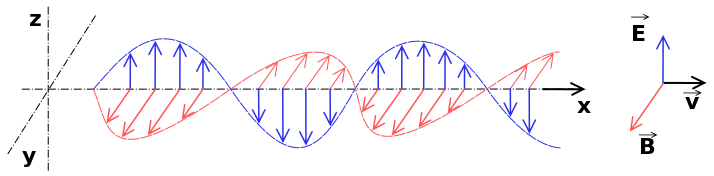
\includegraphics[width=0.8\linewidth]{./pics/ph/wave}
		\end{figure}
		\subsubsection*{Warum breitet sich eine elektromagnetische Welle aus?}
			Aus den mikroskopischen Maxwellgleichungen kann nachvollzogen werden wie J. C. Maxwell auf die Existenz der elektromagnetischen Welle gestoßen ist. Aus der ersten Feldgleichung wird geschlossen, dass ein sich zeitlich veränderndes Magnetfeld, von ringförmigen elektrischen Feldlinien umgeben ist.
			Er folgerte aus dem zweiten Maxwell'schen Feldgesetz: Während sich ein elektrisches Feld ändert, ist es von ringförmigen geschlossenen magnetischen Feldlinien umgeben.
			Somit also: Veränderliche elektrische Felder erzeugen magnetische Wirbelfelder und veränderliche Magnetfelder erzeugen elektrische Wirbelfelder.
			Es ergibt sich also eine Kette von Veränderungen des elektrischen und magnetischen Feldes, die sich als selbstständiges Gebilde im Raum ausbreitet. Ladungen erzeugen elektrische Felder und Ströme erzeugen magnetische Felder.
			Das erste Feldgesetz erweitert diesen Zusammenhang mit Hilfe des zweiten Feldgesetzes nun zu einer beliebig langen Kette:
			\begin{center}
				\large \textbf{Q $ \rightarrow $ E $ \rightarrow $ B $ \rightarrow $ E $ \rightarrow $ ...\\
					\text{ }I  $ \rightarrow $ B $ \rightarrow $ E $ \rightarrow $ B $ \rightarrow $ ...}
			\end{center}
			Elektromagnetische Wellen sind stets Transversalwellen.
			\begin{figure}[h]
				\centering
				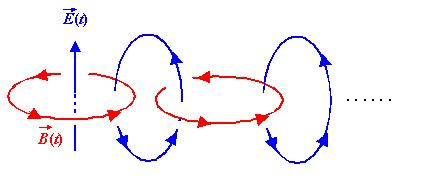
\includegraphics[width=0.3\linewidth]{./pics/ph/trans}
			\end{figure}
		\subsubsection{Quellen von elektromagnetische Wellen}
			\paragraph{Hertzscher Dipol}
				Ein hertzscher dipol ist eine Idealisierung eines Senders elektromagnetischer Strahlung und ist einem offenen elektrischen Schwingkreis äquivalent. Er dient somit als Grundlage für die Berechnung von Antennen.
				\begin{figure}[h]
					\centering
					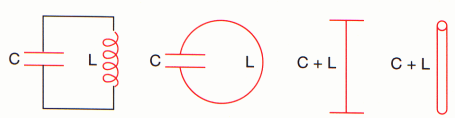
\includegraphics[width=0.6\linewidth]{./pics/ph/hertz}
					\caption{Transformation von einem Schwingkreis zum hertzschen Dipol}
				\end{figure}
				Bei der Transformation wird C und L immer kleiner, wodurch die Resonanzfrequenz steigt. Der hertzsche Dipol emittiert somit hochfrequente elektromagnetische Strahlung.
				\begin{figure}[h]
					\centering
					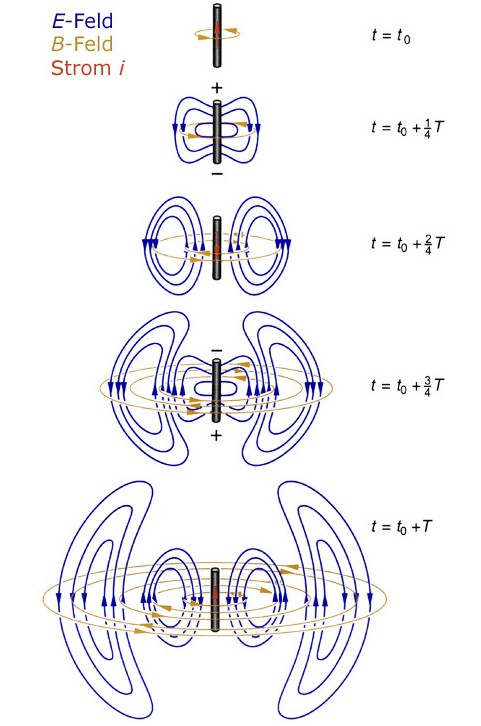
\includegraphics[width=0.4\linewidth]{./pics/ph/hertz2}
					\caption{Ausbreitung der elektromagnetischen Welle eines hertzschen Dipols}
				\end{figure}
			\paragraph{Röntgenstrahlung}
				Röntgenstrahlung kann durch zwei verschiedene Vorgänge entstehen:
				\begin{itemize}
					\item durch starke Beschleunigung geladener Teilchen (meistens Elektronen) -- dies ist die Bremsstrahlung, deren Spektrum kontinuierlich ist --
					\item und durch hochenergetische Übergänge in den Elektronenhüllen von Atomen oder Molekülen. Dies ist die charakteristische Röntgenstrahlung. Sie weist stets ein Linienspektrum auf.
				\end{itemize}
				\begin{tcolorbox}[title=Bremsstrahlung:]
					Wird eine elektrische Ladung beschleunigt, d.h. ändert sich ihr Geschwindigkeitsbetrag bzw. ihre Bewegungsrichtung, so entsteht elektromagnetische Strahlung. Die Energie der dabei auftretenden Photonen ist umso höher, je stärker die Beschleunigung ist.
				\end{tcolorbox}		
				Werden Elektronen auf eine Festkörperoberfläche beschleunigt und in diesem abgebremst, kommt es zu einer Beschleunigung (z.b. Richtungsänderung) durch etwa einen Atomkern. Diese Richtungsänderung führt nach obigem Satz zur Erzeugung von elektromagnetischen Wellen.\\
				Beide Effekte werden in der Röntgenröhre ausgenutzt, in der Elektronen zunächst von einer Glühwendel (Kathode) aus beschleunigt werden (dabei setzen sie keine Röntgenstrahlung frei, weil die Beschleunigung nicht groß genug ist) und anschließend auf die Anode treffen, in der sie stark abgebremst werden. Hierbei entsteht Röntgenstrahlung (Bremsstrahlung, mit insgesamt rund 1\% der eingestrahlten Energie) und Wärme (rund 99\%). Außerdem werden durch Elektronenstöße Elektronen aus den Schalen der Metallatome herausgeschlagen. 
				Ein Elektron wird z. B. durch einen Elektronenstoß aus der K-Schale entfernt und ein Elektron aus der L-Schale fällt in das Loch in der K-Schale. Die Energiedifferenz wird als charakteristische Röntgenstrahlung emittiert.
				\begin{figure}[h]
					\centering
					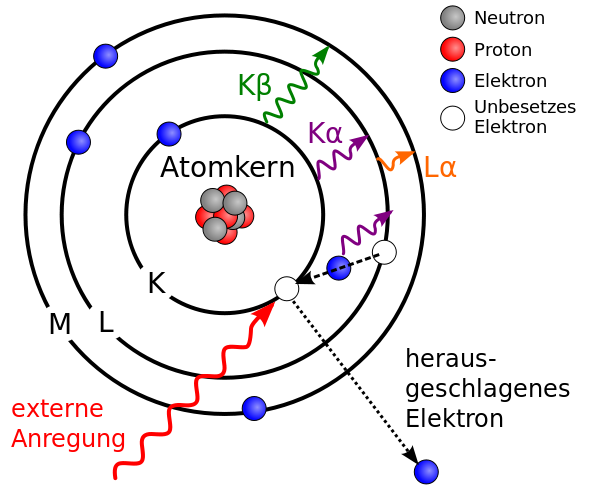
\includegraphics[width=0.4\linewidth]{./pics/ph/roentgen.png}
					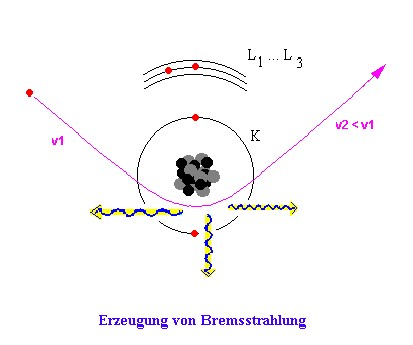
\includegraphics[width=0.4\linewidth]{./pics/ph/brems}
				\end{figure}
				Röntgenstrahlung ist ionisierend. Sie kann dadurch Veränderungen im lebenden Organismus hervorrufen und Schäden bis hin zu Krebs verursachen. Deshalb ist beim Umgang mit der Strahlung der Strahlenschutz zu beachten.
			\paragraph{Wärmestrahlung}	
				Genauso wie in Gasen und Flüssigkeiten eine thermische Molekularbewegung herrscht, haben auch die Atome von Festkörpern eine mirkoskopische kinetische bzw. potentielle Energie. Das heißt sie schwingen um ihre Ruhelagen. Diese mikroskopischen Energien nehmen mit steigender Temperatur zu und schwingen mit höheren Frequenzen. Durch dieses Schwingen von elektrischen Ladungen ändern sich die elektrischen Felder zwischen diesen Ladungen. Es resultiert ein elektrisches Wechselfeld, welches eine elektromagnetische Welle erzeugt, die sich in Form von Wärmestrahlung im Raum ausbreitet.\\
				Die Wärmestrahlung ist eine Art der Wärmeübertragung, bei der Energie anhand elektromagnetischer Wellen (infrarote Strahlung, infrarotes Licht) übertragen wird. Hierbei ist kein Trägermedium erforderlich, so dass also auch Wärme im Vakuum übertragen werden kann. Es ist aber eine direkte Sichtverbindung erforderlich, Hindernisse unterbrechen den Strahlungswärmeaustausch. Schwarze Körper absorbieren ein weites Spektrum an elektromagnetischen Wellen und reflektieren wenig, wodurch sie sich schneller als weiße Körper erwärmen, die mehr Strahlung reflektieren. Die physikalischen Eigenschaften des Materials bestimmen, welche Anteile einer auf das Bauteil auftreffenden Strahlung absorbiert, reflektiert oder transmittiert  werden.
			
				\begin{figure}[h]
					\centering
					\subfigure[Spektrale Energiedichte (abgestrahlte Energie je Wellenlänge) der Wärmestrahlung eines schwarzen Körpers bei verschiedenen Temperaturen]
					{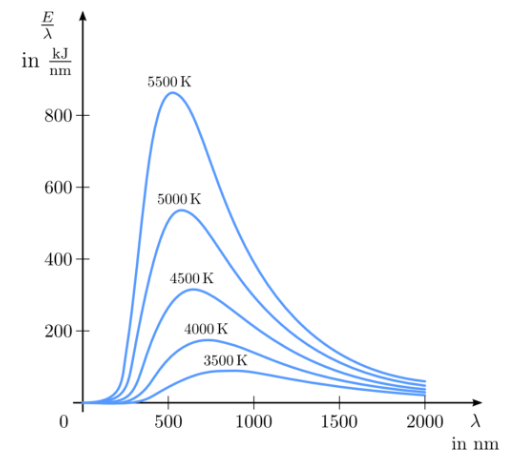
\includegraphics[width=0.45\textwidth]{./pics/ph/waermest}} \hspace{0.4cm}
					\subfigure[Beige Kurve entspricht der Temperatur der Sonne, Rote Kurve entspricht der Umgebungstemperatur] 
					{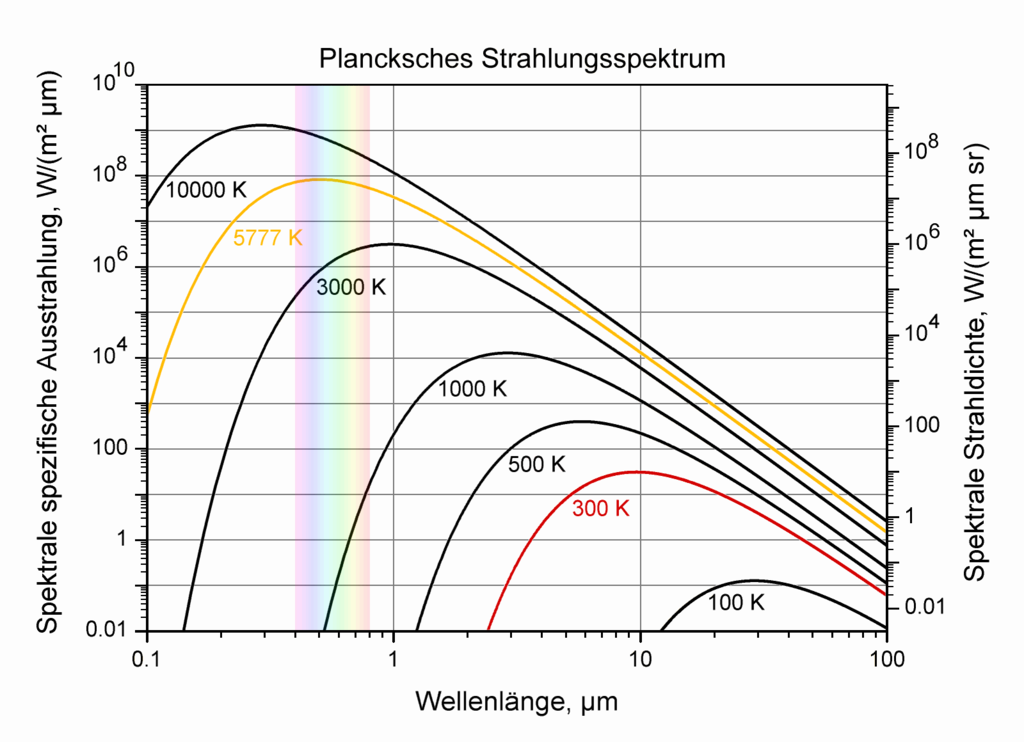
\includegraphics[width=0.45\textwidth]{./pics/ph/waremst}}
				\end{figure}
	\subsection{Welle-Teilchen-Dualismus}
		Der Welle-Teilchen-Dualismus ist eine Erkenntnis der Quantenphysik, wonach den Objekten der Quantenphysik gleichermaßen die Eigenschaften von Wellen, sowie die von  Teilchen zugeschrieben werden müssen. Je nach Art des Experiments tritt entweder der Wellen- oder der Teilchencharakter in Erscheinung, aber niemals beides gleichzeitig.
		\begin{itemize}
			\item Klassische Wellen breiten sich im Raum aus. Sie schwächen oder verstärken sich durch Überlagerung und können gleichzeitig an verschiedenen Stellen mit verschiedener Stärke einwirken.
			\item Ein klassisches Teilchen kann zu einem Zeitpunkt nur an einem bestimmten Ort anwesend sein. Nur dort wirkt es, aber stets mit seiner gesamten Energie, Ladung, Impuls etc.
		\end{itemize}
		Beide Eigenschaften scheinen sich gegenseitig auszuschließen. Trotzdem wurde in mehreren Schlüsselexperimenten für verschiedene Quantenobjekte belegt, dass beide Eigenschaften vorliegen, so dass man jedem Körper eine Materiewelle zuschreibt.\\\\
		Es ist unmöglich, eine anschauliche Vorstellung zu entwickeln, die dem Welle-Teilchen-Dualismus gerecht wird. Die Frage, ob beispielsweise Elektronen oder Lichtquanten „wirklich“ Teilchen oder Wellen seien, ist nicht zu beantworten. Sie sind vielmehr eine eigene Klasse von Quantenobjekten, die je nach der Art der Messung, die man an ihnen durchführt, entweder nur ihre Wellen- oder nur ihre Teilcheneigenschaft in Erscheinung treten lassen, aber nie beide gleichzeitig.\\\\
		Röntgen-, Gamma- und prinzipiell höher energetische Strahlung weist vorwiegend Teilchencharakter auf und niederenergetische Strahlung vorwiegend Wellencharakter.
		
	\subsection{Elektromagnetisches Spektrum}
		\begin{figure}[h]
			\centering
			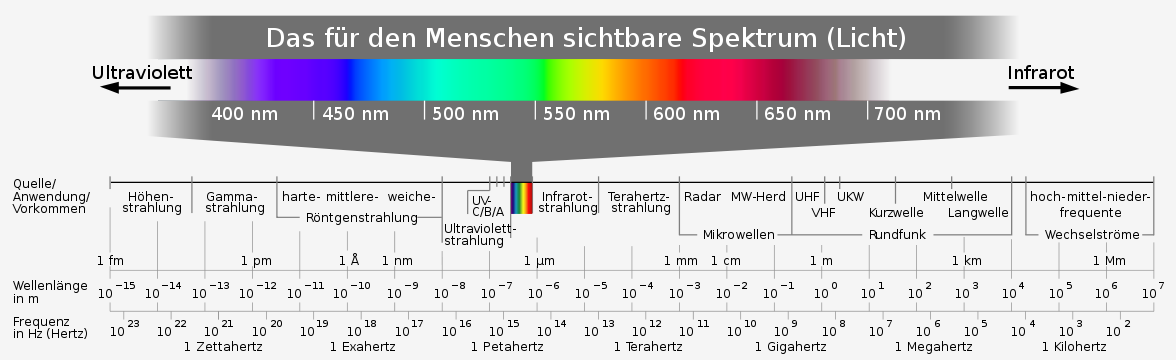
\includegraphics[width=1\linewidth]{./pics/ph/spektrum.png}
		\end{figure}
	
\part{Mathematik}
\section{Allgemeines}
	Bei Differentialgleichungen\\
	Grad: Höchste vorkommende Potenz\\
	Ordnung: Höchste vorkommende Ableitung\\\\
	Bei üblichen Funktionen deuten diese Bezeichnungen beide auf die höchste Potenz in der Funktion hin.
	
\section{Tensorfelder}
	Als Tensorfeld ist eine Abbildung zu verstehen, die jedem Punkt des Raumes eine Zahl, ein Vektor oder eben ein Tensor bestimmter Stufe zuordnet. So wird zum Beispiel der Spannungszustand eines Materials in jedem Punkt durch einen Spannungstensor zweiter Stufe beschrieben. D.h. im 3-dimensionalen Raum wird die Spannung in einem Punkt durch drei $ 3x3 $ Matrizen festgelegt.
	\begin{figure}[h]
		\centering
		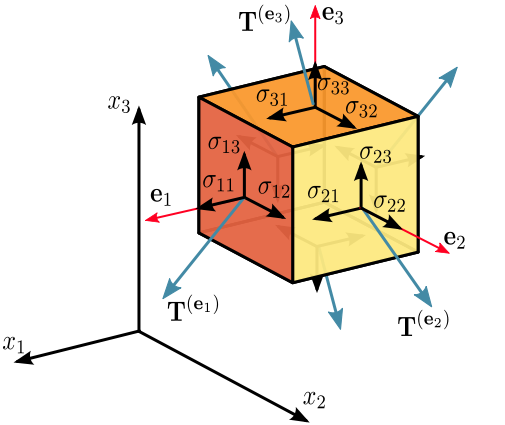
\includegraphics[width=0.4\linewidth]{./pics/ma/spannungstensor}
		\caption{Spannungstensor in der Kontinuumsmechanik}
	\end{figure}
	\leavevmode\\
	
\section{\textcolor{red}{Lineare Algebra}}
\section{\textcolor{red}{Fast Fourier transformation (FFT)}}
	Die FFT ist ein Algorithmus zur effizienten Berechnung der diskreten Fourier-Transformation (DFT). Mit ihr kann ein digitales Signal in seine Frequenzanteile zerlegt und diese dann analysiert werden.
\section{Mathematische Optimierung}
	\subsection{Lineare Optimierung}
		Jedes Problem der linearen Optimierung kann durch eine Zielfunktion
		\[z = \bm{c}^{T}\bm{x}\rightarrow max!\]
		und zugehörige Nebenbedingungen
		\[A\bm{x} \leq \bm{b},\]
		\[\bm{x} \geq 0\]
		formuliert werden.\\\\
		\tab[1cm] \textbf{A} \tab ... \tab $ m\times n- $Matrix mit m Nebenbedingungen und n Variablen inkl. Schlupfvariablen
		\leavevmode \\\\
		Der Lösungsbereich ist immer Polytop (Simplex) und die optimale Lösung befindet sich immer in einer Ecke. Lineare Optimierungsprobleme können deshalb durch Absuchen aller Ecken des zulässigen Bereichs gelöst werden.\\
		\textbf{Satz 1:} Der zulässige Bereich M ist eine konvexe Teilmenge des $ \mathbb{R}^{n} $, d.h. mit zwei Punkten $ \bm{x,y} $ aus M ist auch jede Konvexkombination in M.\\
		\textbf{Satz 2:} Falls der zulässige Bereich M nicht leer und beschränkt ist, so nimmt die Zielfunktion ihr Maximum in mindestens einer Ecke von $ M $ an. \\
		\textbf{Satz 3:} Ein Punkt $ \bm{x} \in M $ ist genau dann eine Ecke von M, wenn die Spaltenvektoren $ a_{j} $ für, welche die zugehörigen Koeffizienten $ x_{j} $ positiv sind, linear unabhängig sind. D.h. für positive $ x_{j} $ müssen die Spalten $ a_{j} $ von A linear unabhängig sein.
		\leavevmode \\\\
		\textbf{Schlupfvariable:} Sie ermöglichen es die Nebenbedingungen statt als Ungleichungen, als Gleichungen anschreiben zu können. Dies beruht auf der Idee, dass die Ungleichung $ x<b $ erfüllt ist, wenn die Gleichung $ x=b-c $ für eine beliebige Zahl $ c>0 $ gilt. Jedes lineare Optimierungsproblem ist in eine solche Normalform überführbar. Die Werte der Schlupfvaraiblen sind für die Lösung des Problems nicht von Interesse.
		\leavevmode \\\\
		\textbf{Erstes Eckenkriterium:} Ist ($ x_{1}, ...,x_{n} $) eine Ecke, dann sind maximal so viele Variablen ungleich von Null, als der Rang der Matrix A (\# NB). Z.b. 3 NB mit zwei Variablen $ x_{1}, x_{2} $ und drei Schlupfvariablen. Eine Ecke kann in diesem Fall maximal drei Variablen ungleich Null besitzen. Sind weniger als drei verschieden von Null, heißt die Ecke entartet. Werden so viele Spalten aus der Matrix A gewählt, dass diese vollen Rang besitzt und damit ein Gleichungssystem angeschrieben, dann ist die Lösung eine zulässige Basislösung wenn alle Variablen größer-gleich Null sind. D.h. wählt man 3 linear unabhängige Spalten von $ \bm{A} $, dann ist dies eine zulässige Basislösung. Andernfalls ist die Basislösung nicht zulässig.\\\\
		Sei $ m $ die Anzahl der Nebenbedingungen (Zeilen von A) und $ n $ die Anzahl der Spalten von A inkl. Schlupfvariablen. Verbleiben nach streichen aller l.a. Spalten noch m=n, dann ist die Lösung eindeutig (1 Punkt mit optimalem Zielfunktionswert). Falls $ \bm{x} $ wenige als $ m $ positive Komponenten hat, so spricht man von einer entartete Ecke.
		\leavevmode \\\\
		\textbf{Zweites Eckenkriterium:} Jede zulässige Basislösung ist eine Ecke. Umgekehrt ist jede nicht entartete Ecke, durch die entsprechenden Spaltennummern eine Basis.
		\leavevmode \\\\
		\textbf{Ein Lösungsalgorithmus:} Man durchlaufe alle Basen aus Spalten der Nebenbedingungsmatrix und berechne zugehörige Basislösungen. Ist diese zulässig, hat man eine Ecke gefunden. Auf diese Weise werden alle Ecken gewonnen. Jene mit dem maximalen Zielfunktionswert ist die optimale Lösung.
		\leavevmode \\\\
		\textbf{Schattenpreise:} Nach einer gefundenen Lösung soll erörtert werden, ob der Zielfunktionswert weiter erhöht werden kann indem die optimale Lösung (Ecke) leicht variiert wird (Beschränkungen in $ \bm{b} $ ändern). Jede Nebenbedingung (i) hat einen Schattenpreis $ \Delta z = \Delta z(i) $, um den sich der Gewinn erhöht, wenn die Beschränkung der entsprechenden Ressource um eine Einheit erhöht wird. Die Beschränkungen werden durch den Vektor $ \bm{b} $ beschrieben.
		\leavevmode \\\\
		\textbf{Sensitivitätsanalyse der Zielfunktion:} Es wird untersucht, in welchem Rahmen die Koeffizienten der Zielfunktion variiert werden können, ohne die gewonnene optimale Lösung zu ändern.
		\leavevmode \\\\
		\textbf{Sensitivitätsanalyse der Einsatzmittelbeschränkung:} Es wird untersucht, in welchem Rahmen die Koeffizienten des Vektors $ \bm{b} $ geändert werden können, sodass die gewählte Basislösung zulässig ($ \bm{x}(i) \geq 0 $) bleibt.
		\leavevmode \\\\
		Das Lösen der Zielfunktion zu einem Optimum wird \textit{primales Problem} genannt. Die Schattenpreise sind die Lösungen des \textit{dualen Problems} oder können auch als sogenannte Lagrangemultiplikatoren erhalten werden.
		\[Z = \bm{b}^{T}\bm{u}\rightarrow min,\]
		\[A^{T}\bm{u} \geq \bm{c},\]
		\[\bm{u} \geq 0\]
		Zielfunktionswerte des primalen und dualen Problems stimmen stets überein. Es gilt
		\[z = \bm{c}^{T}\bm{x} = \bm{b}^{T}\bm{u} = Z.\]
		Daraus folgt, dass die Komponenten von $ \bm{u} $ gerade die Schattenpreise $ \Delta z(i) $ sind. Erhöht man nämlich $ b_{i} $ um eine Einheit, unter Beibehaltung der zulässigen Basis, dann ergibt sich gerade
		\[z_{neu} = \bm{b}^{T}_{neu}\bm{u} = \underbrace{\bm{b}^{T}_{alt}\bm{u}}_{z_{alt}} + \underbrace{1\cdot u_{i}}_{\Delta z}.\]
		\leavevmode \\
		\textbf{Voragangsweise bei Gleichheitsnebenbedingungen:} Falls nicht $ m $ Schlupfvariablen auftreten, müssen stattdessen Hilfsvariablen eingeführt werden um eine Startecke zu finden. In der optimalen Lösungen müssen alle Spalten von Hilfsvariablen mit solchen der ursprünglichen Matrix $ \bm{A} $ getauscht sein, sonst hat das Problem keine Lösung. Man streicht dann die hinteren Spalten, nach Anzahl der eingeführten Hilfsvariablen und erhält eine neue Matrix $ \bm{A} $ mit einer Einheitsmatrix am Anfang. 
		\leavevmode \\\\
		\textbf{Simplexalgorithmus:}
		
		
	\subsection{Ganzzahlige Lineare Optimierung}
		Ein solches Problem wird über Ressourcen $ R_{1}, ...,R_{h} $ und Jobs $ J_{1}, ...,J_{k} $, denen Ressourcen zugeteilt werden können beschrieben. Bekannt seien die Kosten $ c_{ij} $ einer Ressource für einen bestimmten Job. Gesucht ist der optimale, kostengünstigste Zuordnungsplan, bei dem jede Ressource höchstens einen Job und jeder Job von höchstens einer Ressource bearbeitet wird. \\
		Da der Rechenaufwand für das Auffinden aller optimalen Lösungen sehr groß werden kann, wird über das \textit{Branch-and-Bound-Verfahren} ein reduzierter Entscheidungsbaum erstellt.
		\begin{figure}[h]
			\centering
			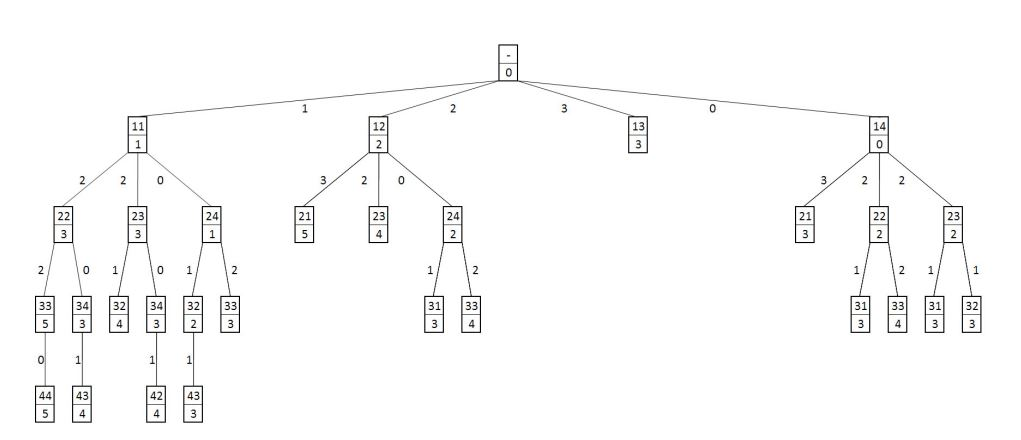
\includegraphics[width=0.7\linewidth]{./pics/ma/bnd} 
			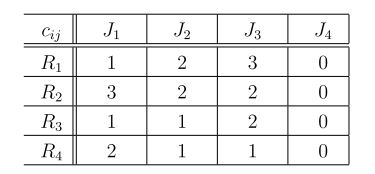
\includegraphics[width=0.29\linewidth]{./pics/ma/bndt}
		\end{figure}
		\leavevmode \\
		Ein Zweig wird terminiert, falls längs diese Zweigs kein niederer Zielfunktionswert erzielt werden kann. Oben im Knoten ist die Indexierung und unten der Zielfunktionswert eingetragen. An den Kanten sind die Kosten aufgetragen.
		\leavevmode \\\\
		\textbf{Rucksackproblem}\\
		Gegeben sind $ n $ Ausrüstungen mit Gewichten $ g_{1}, ...,g_{n} $ und den Werten $ w_{1}, ..., w_{n} $. Gesucht ist die Kombination an Ausrüstung mit dem maximalen Gesamtwert $ W $, deren Gesamtgewicht unterhalb einer vorgeschriebenen Grenze $ G $ ist. Zur Formulierung ob der Gegenstand gewählt wurde, wird $ x_{j} = 1 $ und falls nicht $ x_{j} = 0 $ gesetzt.
		\[W = \sum_{j=1}^{n} w_{j}x_{j}\rightarrow max\]
		\[\sum_{j=1}^{n} g_{j}x_{j} \leq G\]
		Gestartet wird mit der Summe der Werte aller Gegenstände $ W_{O} = \sum_{j=1}^{n} w_{j} $ und einer unteren Gewichtsschranke $ G_{0} = 0 $. Wird ein Gegenstand ausgewählt ($ x_{j} = 1 $), dann wird zur unteren Gewichtsschranke $ G_{U} $ das Gewicht $ g_{j} $ hinzu addiert. Falls der Gegenstand nicht verwendet wird ($ x_{j} = 0 $), dann wird der maximal erreichbare Gesamtwert $ W $ um den Wert $ w_{j} $ verringert. Ein Zweig wird terminiert, wenn die untere Gewichtsschranke die vorgegebene Gewichtsschranke überschreitet $ G_{U} > G $ oder wenn eine neue obere Wertschranke $ W_{O} $ kleiner wird als der aktuelle Gesamtwert $ W_{A} $.
		\begin{figure}[h]
			\centering
			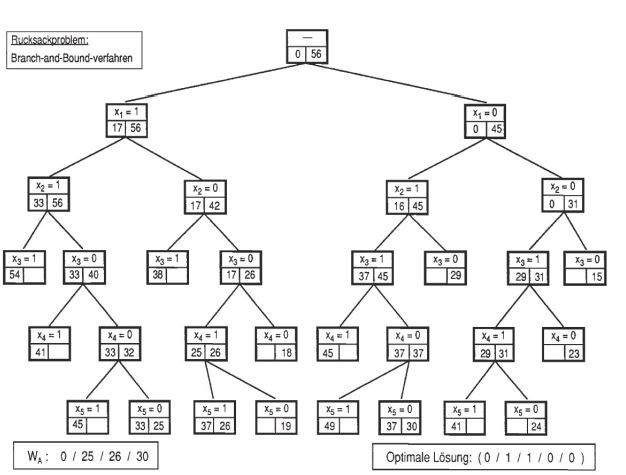
\includegraphics[width=0.6\linewidth]{./pics/ma/rucksack}
			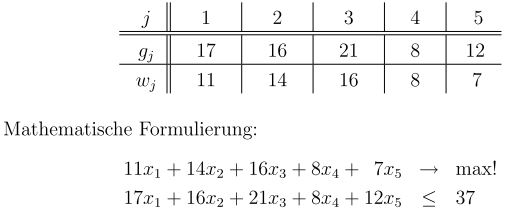
\includegraphics[width=0.39\linewidth]{./pics/ma/rucksackt}
		\end{figure}
		\leavevmode \\\\
		\textbf{Das Allgemeine Problem, Dakin-Verfahren}\\
		Das allgemeine ganzzahlige Optimierungsproblem hat die Form
		\[W = \sum_{j=1}^{n}c_{j}x_{j} \rightarrow max\]
		\[\sum_{j=1}^{n} a_{ij}x_{j} \leq b_{j}\]
		\[x_{j} \geq 0,\text{ } und\text{ } ganzzahlig.\]
		Das Problem wird in mehrere Teilprobleme aufgespalten. Als erstes wird die Ganzzahligkeitsanforderung weggelassen und eine möglicherweise nichtganzzahlige Ecke aus den Nebenbedingungen berechnet. Ebenso der zugehörige Zielfunktionswert, der ebenfalls nichtganzzahlig sein kann.\\
		Diese Lösung wird aufgespalten, indem man die erste nichtganzzahlige Variable nimmt und die größte ganzzahlige Zahl $ x_{j} $ nennt. Z.b. von 3.75 $ \rightarrow x_{j} = 3 $. Über die jeweilige NB werden dann die restlichen Variablen berechnet. Sind alle Variablen ganzzahlig, wird terminiert. Sind jedoch noch nicht alle Variablen ganzzahlig, wird weiter aufgespalten. Man nimmt die nächste nichtganzzahlige Variable und rundet diese wieder einmal \textit{floor} und \textit{ceil}. Z.b. aus 1.2 $ \rightarrow $ 1 und 2. Falls die Variablen die zugehörige NB verletzen, wird terminiert. Falls das Wählen der zweiten Variable zur Ganzzahl die erste Varaible wieder nichtganzzahlig macht, wird erneut aufgespalten. Dies wird solange iteriert bis alle Zweige terminiert sind. Eine weitere Terminierungsbedingung ist, wenn eine nichtganzzahlige Lösung vorliegt und der zugehörige Zielfunktionswert kleiner als größte bereits bekannte Zielfunktionswert einer zulässigen Lösung ist.
		\begin{figure}[h]
			\centering
			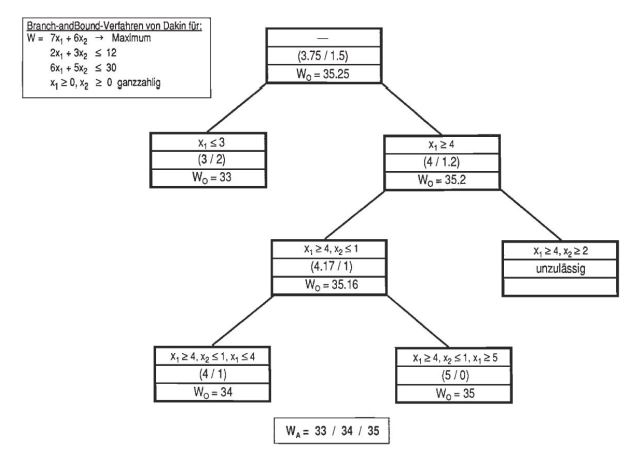
\includegraphics[width=0.7\linewidth]{./pics/ma/dak}
			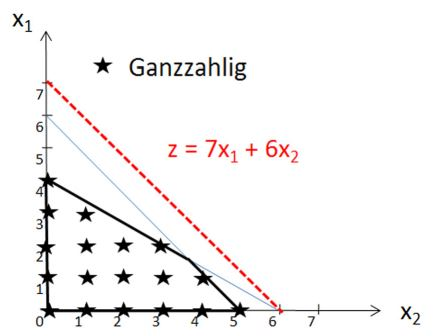
\includegraphics[width=0.29\linewidth]{./pics/ma/dakd}
		\end{figure}
		\leavevmode \\\\
		\textbf{Das Reihenfolgeproblem, Johnson-Algorithmus (\textit{greedy-algorithm})}\\
		Es seien $ n $ Jobs gegeben die hintereinander auf Maschine $ M_{1} $ und dann auf $ M_{2} $ erledigt werden müssen. Die Bearbeitungszeit des Jobs $ j $ sei auf $ M_{1} $ sei $ a_{j} $ und auf $ M_{2} $, $ b_{j} $. Gesucht ist der optimale Belegungsplan, der die optimale Reihenfolge mit der kürzesten benötigten Gesamtzeit aufweist (äquivalent: kürzeste Standzeiten der Maschinen).\\\\
		Für zwei Maschinen liefert der Johnson-Algorithmus eine exakte Lösung. Bei mehreren Maschinen bzw. komplizierteren Arbeitsabläufen kann das Problem als allgemeine ganzzahlige Optimierungsaufgabe gestellt  und mit dem Dakin-Verfahren gelöst werden.\\\\
		Man suche $ min(a_{1}, ...,a_{n},b_{1}, ...,b_{n}) $. Ist der kürzeste Arbeitsschritt $ a_{j} $, wird der Job $ j $ als Erstes abgearbeitet. Ist der kürzeste Arbeitsschritt $ b_{j} $, dann wird der Job $ j $ als letztes abgeschlossen. Dann wird Job $ j $ gestrichen und der Vorgang beginnt von vorne, bis man die optimale Reihenfolge der Jobs gefunden hat.
	
	\subsection{Globale Optimierung}
		Die allgemeine Aufgabe besteht darin, eine Funktion $ f $ über eine abgeschlossene Teilmenge $ D $ zu minimieren.
		\[f(x) \rightarrow min, \quad x\in D\]
		$ D $ wird durch Nebenbedingungen in Form von Gleichungen und Ungleichungen gegeben. Maximierungsaufgabe ist wegen $ max(f) = -min(-f) $ ebenfalls abgedeckt. Falls die Gleichungen differenzierbar sind, bietet sich die Methode der \textit{Lagrangemultiplikatoren} an.
		\leavevmode \\\\
		\textbf{Lagrangemultiplikatoren, NB als Gleichungen}\\
		Für eine gegebene differenzierbare Funktion $ f $ soll die Minimierungsaufgabe
		\[f(x) \rightarrow min\]
		unter den Nebenbedingungen
		\[g_{1}(x)=0, ...,g_{k}(x)=0\]
		gelöst werden, wobei die NB differenzierbar und ihre Gradienten
		\[\nabla g_{1}(x), ...,\nabla g_{k}(x)\]
		als linear unabhängig vorausgesetzt werden. Die \textit{Lagrangemultiplikatorregel} wird wie folgt angewendet.\\\\
		\textit{1. Schritt:} Man bilde die Hilfsfunktion in n+k Variablen $ x_{1}, ...,x_{n},u_{i}, ...,u_{k} $
		\[L(\bm{x},\bm{u}) = f(\bm{x}) + \bm{u}^{T}\bm{g}(\bm{x})\]
		und berechne die Gradienten der Hilfsfunktion.\\\\
		\textit{2. Schritt:} Man bestimmte die stationären Punkte der Lagrangefunktion. Das sind die Lösungen des Gleichungssystems 
		\[\nabla L(x_{1}, ...,x_{n},u_{i}, ...,u_{k}) = \bm{0}.\]
		Das heißt,
		\[\frac{\partial}{\partial x_{i}} L = \frac{\partial}{\partial x_{i}}f(\bm{x}) + u_{1}\frac{\partial}{\partial x_{i}}g_{1(x)}+ ... + u_{k}\frac{\partial}{\partial x_{i}}g_{k}(\bm{x})\]
		\[\frac{\partial}{\partial u_{j}}L = g_{j}(\bm{x}) = \bm{0}\]
		für $ i = 1, ...,n $ und $ j = 1, ...,k $\\\\
		\textit{3. Schritt:} Die Maxima und Minima sind unter den Lösungen ($ x_{1}, ..., x_{n} $) zu finden.
		\leavevmode \\\\
		\textbf{Lagrangemultiplikatoren, NB als Ungleichungen}\\
		Liegen die Nebenbedingungen als Ungleichungen vor,
		\[f(x) \rightarrow min\]
		\[\bm{g(x)} \leq \bm{0}, \quad \bm{x} \geq \bm{0} \]
		so bildet man ebenfalls die Lagrangefunktion
		\[L(\bm{x},\bm{u}) = f(\bm{x}) + \bm{u}^{T}\bm{g}(\bm{x}).\]
		Anstelle des Aufsuchens der stationären Punkte der Lagrangefunktion sind jetzt die Sattelpunkte zu ermitteln. Ein Paar ($ \bm{x,u} $) mit $ \bm{x} \geq \bm{0}, \quad \bm{u} \geq \bm{0} $ heißt Sattelpunkt, falls
		\[L(x,v) \leq L(x,u) \leq L(y,u)\]
		für alle $ (\bm{y,v}) $ mit $ \bm{y} \geq \bm{0}, $  $ \bm{v} \geq \bm{0} $ erfüllt ist. Das heißt ($ \bm{x,u} $) ist ein Sattelpunkt wenn der Funktionswert beim Verlassen des Punktes in \textit{v-Richtung} abnimmt ($ L(x,v) $) und in \textit{y-Richtung} zunimmt ($ L(y,u) $).
		\subsubsection{Quadratische Optimierung}
			Das quadratische Standardproblem ist
			\[f(\bm{x}) = \bm{x}^{T}\bm{Ax} - \bm{b}^{T}\bm{x}\]
			mit einer symmetrischen und positiv definiten Matrix $ \bm{A} $. Das Lösen des linearen Gleichungssystems $ \bm{Ax} = \bm{b} $ ist äquivalent und führt zum selben Ergebnis. Denn der Gradient ist
			\[\nabla f(\bm{x}) = \bm{Ax}-\bm{b}.\]
			\textit{Vorkonditionierung:} Eine Matrix $ \bm{B} $ zur Vorkonditionierung dient dazu die Kondition, also die Abhängigkeit der Lösung von den Eingangsdaten, zu verringern.\\\\
			Eine Iteration kann dann folgendermaßen geschrieben werden, wobei $ \alpha $ die Distanz in die Abstiegsrichtung $ \bm{s}_{k} $ bis zur nächsten Iteration $ \bm{x}_{k+1} $ beschreibt.
			\[\bm{x}_{k+1} = \bm{x}_{k} + \alpha \bm{s}_{k}, \qquad \bm{Bs}_{k} = \bm{b} - \bm{Ax}_{k} \quad \Rightarrow \quad \bm{s}_{k} = -\bm{B}^{-1}\nabla f(\bm{x}_{k}) \]
			Bei der \textit{konjugierten Gradienten Methode} wird die Abstiegsrichtung $ \bm{p}_{k} $ nochmals mit dem Relaxationsfaktor $ \beta_{k} $ korrigiert, um ein Optimum in weniger Iterationen zu finden.
			\[\bm{p}_{k} = \bm{s}_{k} + \beta_{k}\bm{p}_{k-1} \]
			Sobald der Betrag des Gradienten eine gewisse Toleranz unterschreitet werden die Verfahren abgebrochen.
		\subsubsection{Lineare kleinste Fehlerquadrate}
			Das Problem überbestimmter linearer Systeme und die Minimierung der Summe der Fehlerquadrate ist
			\[f(\bm{x}) = ||\bm{Ax}-\bm{b}||^{2} \rightarrow min.\]
			Man kann auch
			\[f(\bm{x}) = (\bm{Ax}-\bm{b})^{T}(\bm{Ax}-\bm{b}) = \bm{x^{T}A^{T}Ax} - 2\bm{x^{T}A^{T}b} + \bm{b^{T}b} \]
			schreiben. Über die partiellen Ableitungen, den Gradienten 
			\[\nabla f(\bm{x}) = 2\bm{A^{T}Ax} - 2\bm{A^{T}b}\]
			und der Bedingung, dass dieser zu Null wird, können die gesuchten Parameter $ \bm{x} $ über das lineare Gleichungssystem
			\[\bm{A}^{T}\bm{Ax} = \bm{A}^{T}\bm{b}\]
			berechnet werden. Die Bedingung $ \nabla f(\bm{x}) = \bm{0} $ folgt aus der Forderung das Fehlerquadrat zu minimieren. Da das Fehlerquadrat in jedem Punkt konstant ist, ergibt sich in den partiellen Ableitungen jedes Punktes, dieser Wert zu Null.
		\subsubsection{Nichtlineare kleinste Fehlerquadrate}
			Eine Idee ist dieses nichtlineare Problem als eine Abfolge von linearen kleinsten Fehlerquadraten iterativ zu Lösen. Die nichtlineare Funktion $ \bm{F(x)} $ wird über die Taylor-Entwicklung durch quadratische Funktionen angenähert, die wiederum zum Lösen des linearen Gleichungssystems $ \bm{Ax} - \bm{b} $ äquivalent sind (\textit{Gauss-Netwon Verfahren}). Der Vorteil ist, dass die oft schwierig zu berechnenden zweiten Ableitungen nicht benötigt werden.
			\[\bm{F(x)} \approx \bm{F(x^{k})} + \bm{J}_{F}(\bm{x}^{k})(\bm{x} - \bm{x}^{k}) \]
			Der nächste Iterationsschritt wird durch Lösung des Minimierungsproblems
			\[f(\bm{x}) = ||\bm{F(x^{k})} + \bm{J}_{F}(\bm{x}^{k})(\bm{x} - \bm{x}^{k})||^{2} \rightarrow min\]
			gewonnen. Mit $ \bm{A} = \bm{J}_{F}(\bm{x}^{k}), $ $ \bm{s}^{k} = \bm{x-x}^{k} $ und $ \bm{b} = -\bm{F(x^{k})} $ erhalten wir das Problem der linearen kleinsten Fehlerquadrate
			\[||\bm{As}^{k} - \bm{b}||^{2}\rightarrow min \]
			Verbesserte Varianten beheben das Problem, dass sich die Summe der Fehlerquadrate nicht mit jeder Iteration verringern. Das Problem liegt bei $ \alpha $ der in Abstiegsrichtung ein zu großes Inkrement verweist. Dafür ist ein \textit{line search} notwendig, das die Zielfunktion in Abstiegsrichtung minimiert. Auch bei der \textit{trust region Gauss-Newton} Methode geht es darum, die \textit{sufficient decrease condition} zu erfüllen. Durch das folglich reduzierte auswerten von Funktionswerten wird der Algorithmus effizienter und benötigt weniger Iterationsschritte.
		\subsubsection{Ableitungsfreie Methoden}
			\textbf{Koordinatensuch-Methoden}\\
			Sie basieren auf der Suche von Funktionswerten anhand eines Rasters auf dem die Zielfunktion ausgewertet wird. Schritt für Schritt bewegt man sich mit dem Raster in Richtung absteigender Zielfunktionswerte. Wird kein kleinerer Zielfunktionswert auf dem Raster gefunden, wird das Raster verfeinert. Um die Wahrscheinlichkeit eines Verfangens in lokalen Minimas zu verringern werden zufällig gewählte Startwerte durchprobiert und der Algorithmus durchgeführt. Man wählt dann denn kleinsten Zielfunktionswert aus allen \textit{runs}.
			\leavevmode\\\\
			\textbf{Downhill-Simplex-Methode}\\
			Die Startkonfiguration ist eine Selektion aus $ n+1 $ Punkten $ \mathbb{R}^{n} $. \\
			Schritt1: Diese Punkte sind nach ihren Funktionswerten (beste $ \rightarrow $ schlechtester) geordnet. In einer Iteration wird der schlechteste Punkt durch Reflexion, Expansion oder Kontraktion ausgetauscht.\\
			Schritt 2: Berechne den Mittelpunkt des Dreiecks.\\
			Schritt 3: Zuerst wird der reflektierte Punkt mit dem schlechtesten Funktionswert berechnet. Ist der reflektierte Punkt besser als der Beste, dann berechne den expandierten Punkt (Schritt 4) und ersetzte den schlechtesten durch den besseren (Reflexion oder Expansion). Zurück zu Schritt 1. Ist der reflektierte Punkt nur besser als der zweitschlechteste, dann ersetzte den schlechtesten durch den Reflektierten. Zurück zu Schritt 1.\\
			Schritt 5: Falls der reflektierte Punkt nicht besser als der Zweitschlechteste (Mittlere) ist, dann berechne den kontrahierten Punkt. Falls dieser besser als der Reflektierte ist, dann ersetzte den schlechtesten durch diesen. Zurück zu Schritt 1.\\
			Schritt 6: Wird durch Reflexion, Expansion oder Kontraktion kein besserer Funktionswert mehr erreicht, kann durch Reduktion aller Punkte zum besten hin, der Zielfunktionswert noch verbessert werden.
			\leavevmode\\\\
			\textbf{Simmulierte Abkühlung}\\
			Grundidee ist die Nachbildung eines Abkühlungsprozesses, etwa beim Glühen in der Werkstoffkunde. Nach Erhitzen eines Metalls sorgt die langsame Abkühlung dafür, dass die Atome ausreichend Zeit haben, sich zu ordnen und stabile Kristalle zu bilden. Dadurch wird ein energiearmer Zustand nahe am Optimum erreicht. \\
			Es wird ein Startwert $ \bm{x} $ und eine Temperaturfolge die gegen Null fällt gewählt. Der Wert wird mit einem Nachbarspunkt $ \bm{y} $ verglichen $ \Delta f = f(\bm{x}_{0})-f(\bm{y}) $.\\
			Falls $ \Delta f > 0 $ dann wird $ \bm{x}_{1}=\bm{y} $ gewählt.\\
			Falls $ \Delta f \leq 0 $ dann wird nur mit einer Wahrscheinlichkeit der Punkt $ \bm{x}_{1}=\bm{y} $ übernommen und mit einer Gegenwahrscheinlichkeit wird der Schritt erneut mit einem anderen Nachbarspunkt ausgeführt.\\
			Dies wird für jeden Temperaturschritt durchgeführt.\\
			\textit{Verdeutlichung: } Angenommen, man sucht in einer zweidimensionalen Landschaft den (global) tiefsten Punkt. Die Landschaft selbst besteht aus vielen unterschiedlich tiefen Dellen. Die einfache Suchstrategie (suche den nächsten tiefsten Punkt) entspricht dem Verhalten einer Kugel, welche in dieser Landschaft ausgesetzt wird. Sie rollt zum nächsten lokalen Minimum und bleibt dort. Bei der simulierten Abkühlung wird der Kugel immer wieder ein Stoß versetzt, der mit zunehmender „Abkühlung“ schwächer wird. Dieser ist idealerweise stark genug, um die Kugel aus einer flachen Delle (lokales Minimum) zu entfernen, reicht aber nicht aus, um aus dem globalen Minimum zu fliehen.
			\leavevmode\\\\
			\textbf{Surrogate-Modelling}\\
			Es werden einfachere Modelle verwendet, die die Optimierungsfunktion annähern. Es wird dann diese Näherung optimiert.\\
			Beispielsweise kann eine echte Optimierungsfunktion durch kubische Splines interpoliert werden. Man kann dann für jeden lokalen Spline das Optimum berechnen und erhält somit auch das genäherte Optimum der Zielfunktion.
			\leavevmode\\\\
			\textbf{Genetische Algorithmen}\\
			Diese Algorithmen ahmen natürliche Selektion nach.  
			\begin{itemize}
				\item Es wird mit einem Set von \textit{Parents} gestartet. $ \bm{P} = [x_{1}, ..., x_{n}] $
				\item Für jeden Parent wird eine Fitness berechnet. $ F(x_{1}), ..., F(x_{n}) $
				\item Bis ein Abbruckkriterium erfüllt ist
				\begin{itemize}
					\item Selektion und Rekombination von Individuen anhand von Fitnesswerten 
					\item Mutation
					\item Fitnessevaluation
					\item Selektion einer neuen Generation
				\end{itemize}
			\end{itemize}
			\leavevmode
			\textbf{Partikelschwarm-Optimierung}\\
			Als Partikelschwarmoptimierung (PSO) wird ein naturanaloges Optimierungsverfahren bezeichnet, das nach dem Vorbild des biologischen Schwarmverhaltens eine Lösung für ein Optimierungsproblem sucht. Analog zum natürlichen Phänomen wird eine Population von Lösungskandidaten durch den Suchraum bewegt, um eine gute Lösung für das Problem zu erhalten. In jedem Rechenschritt wird dazu die Position jedes Individuums und der zugehörige Funktionswert neu berechnet. Beim Schwarm haben die Nachbarn Einfluss auf ein Individuum. Voraussetzung ist ebenfalls das der Schwarm zusammenhält.
			\leavevmode\\\\
			\textbf{Neuronale Netzwerke}\\
			Ein neuronales Netz besteht aus einer Eingangsschicht, einer oder mehrerer Schichten aus künstlichen Neuronen (Übertragungsfunktionen) und einer Ausgangsschicht. Nach der Konstruktion eines Netzes folgt die Trainingsphase. Beim Lernen werden neue Verbindungen gesetzt, gelöscht, die Gewichtung verändert, Schwellwerte angepasst oder ganze Neuronen hinzugefügt oder gelöscht. Jedes Neuron hat demnach einen Threshold ab dem es aktiviert wird und ein Gewicht mit dem der Eingang, dem Ausgang übergeben wird.
			
	\subsection{Konvexe Optimierung}
		Der zentrale Standardfall der nichtlinearen Optimierung ist die konvexe Optimierung, bei der die Funktion $ f $ und $ g_{i} $ als konvex vorausgesetzt werden. $ f $ heißt \textit{konvex}, wenn der Graph unterhalb der Verbindungsgeraden, zweier auf der Funktion liegende Punkte, verläuft.
		\begin{figure}[h]
			\centering
			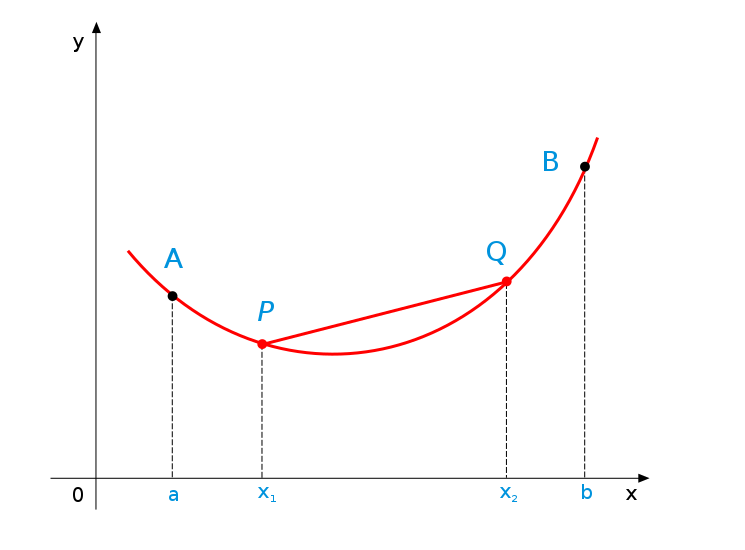
\includegraphics[width=0.3\linewidth]{./pics/ma/konvex}
		\end{figure}
		\[f(\mu \bm{P} + (1-\mu)\bm{Q}) \leq \mu f(\bm{P}) + (1-\mu)f(\bm{Q}), \quad 0\leq \mu \leq 1  \]
		\leavevmode \\
		Die NB sind Ungleichungen. Es kann jedoch aus $ g_{j} \leq 0 $ und $ -g_{j} \leq 0 $, eine Gleichheitsnebenbedingung $ g_{j} = 0 $ gebildet werden. Falls die definierende Ungleichung strikt ($ < $ statt $ \leq $) ist, so heißt die Funktion \textit{streng konvex}. Eine partiell differenzierbare Funktion ist genau dann konvex, wenn für alle $ \bm{x,y} $ gilt
		\[f(\bm{y}) \geq f(\bm{x}) + (\bm{y}-\bm{x})^{T}\nabla f(\bm{x}).\]
		Das heißt, wenn ihr Graph für jeden Punkt oberhalb der zugehörigen Tangente verläuft. Für das Lösen eines konvexen Optimierungsproblems gehen wir davon aus, dass alle beteiligten Funktionen $ f $ und $ g_{i} $ konvex sind. Die NB können in einem Vektor $ \bm{g(x)} = [g_{1}(\bm{x}), ..., g_{m}(\bm{x})]^{T} $ zusammengefasst werden und führen den konvexen zulässigen Bereich ein, der durch die NB definiert wird.
		\[M = \{\bm{x} \in \mathbb{R}^{n}: \bm{g(x)} \leq \bm{0}, \bm{x} \geq \bm{0}\}\]
		Zur Lösung des Optimierungsproblems wird die \textit{Lagrangefunktion} mit den \textit{Lagrangemultiplikatoren} $ u_{j} $ gebildet
		\[L(\bm{x},\bm{u}) = f(\bm{x}) + \bm{u}^{T}\bm{g}(\bm{x}) = f(\bm{x}) + \sum_{j=1}^{m}u_{j}g_{j}.\]
		\textbf{Satz:} Falls ein Paar $ (\bm{x,u}) $ ein Sattelpunkt der \textit{Lagrangefunktion} $ L $ ist, so ist $ \bm{x} $ die Lösung der Minimierungsaufgabe.\\\\
		\textit{Slater-Bedingung:} Falls der zulässige Bereich $ M $ innere Punkte $ \bm{x'} $ besitzt, d.h. falls es mindestens ein $ \bm{x'} \geq \bm{0}$ gibt für den $ \bm{g(x')} < \bm{0} $ gilt. \\\\
		\textbf{Theorem von Kuhn-Tucker:} Falls $ M $ die \textit{Slater-Bedingung} erfüllt, dann ist $ \bm{x} \geq \bm{0} $ genau dann eine Lösung des Minimierungsproblems, wenn es ein $ \bm{u} \geq \bm{0} $ gibt und das Paar $ (\bm{x,u}) $ ein Sattelpunkt von $ L $ ist.
		\[\frac{\partial L}{\partial \bm{x}} \geq 0, \quad \bm{x}^{T}\partial_{x} L(\bm{x,u}) = 0, \quad \bm{x} \geq \bm{0} \]
		\[\frac{\partial L}{\partial \bm{u}} \leq 0, \quad \bm{u}^{T}\partial_{u} L(\bm{x,u}) = 0,  \quad \bm{u} \geq \bm{0}\]
		Man muss also für eine Funktion $ f $ und die NB in Form von Ungleichungen prüfen ob die obigen Kuhn-Tucker Bedingungen, sowie $ \bm{x} \geq \bm{0} $, $ \bm{u} \geq \bm{0} $ erfüllt sind. Sind die Kuhn-Tucker Beidngungen erfüllt, dann ist $ (\bm{x,u}) $ ein Sattelpunkt und $ \bm{x} $ somit eine Lösung des Minimierungsproblems.
		\leavevmode \\\\
		\textbf{Quadratische Optimierung mit Kuhn-Tucker}\\
		Das Standardproblem der quadratischen Optimierung mit linearen NB ist
		\[f(\bm{x}) = \bm{x}^{T}\bm{Cx} + \bm{c}^{T}\bm{x} \rightarrow min\]
		\[\bm{Ax} \leq \bm{b}, \quad \bm{x} \geq \bm{0}.\]
		Mit positiv semidefiniter ($ \bm{x}^{T}\bm{Cx} \geq 0 $) Matrix $ \bm{C} $. Die \textit{Lagrangefunktion} ist dann
		\[L(\bm{x,u}) = \bm{x}^{T}\bm{Cx} + \bm{c}^{T}\bm{x} + \bm{u}^{T}(\bm{Ax} - \bm{b}).\]
		Die zugehörigen Gradienten werden als $ \bm{v} $ und $ \bm{-y} $ definiert
		\[\partial_{x} L(\bm{x,u}) = 2\bm{Cx} + c + \bm{A}^{T}\bm{u} =: \bm{v},\]
		\[\partial_{u} L(\bm{x,u}) = \bm{Ax} - \bm{b} =: \bm{-y}\]
		Die Sattelpunktbedingungen werden dann über die Kuhn-Tucker Bedingungen als
		\[\bm{v} \geq \bm{0}, \quad \bm{x}^{T}\bm{v} = 0,\]
		\[\bm{y} \geq \bm{0}, \quad \bm{u}^{T}\bm{y} = 0,\]
		formuliert.
	\subsection{Variationsrechnung}
		Ein Funktional ist eine Funktion, die anderen Funktionen Zahlen zuordnet. Es ist also eine Abbildung $ \phi : M \rightarrow \mathbb{R} $ von einer Funktionenmenge in die reellen Zahlen. Ein Funktional ordnet also jeder Funktion $ u \in M $ eine Zahl $ \phi(u) $ zu. Ziel der Variationsrechnung ist die Minimierung solcher Funktionale.\\\\
		\textit{Fundamentallemma der Variationsrechnung:} Ist $ f $ eine stetige Funktion und $ \int_{x_{0}}^{x_{1}}f(x)v(x)dx = 0 $ für alle stetigen Funktionen $ v $ und auch $ v(x_{0}) = v(x_{1}) = 0 $, dann ist auch $ f(x) = 0 $ für alle $ x \in [x_{1},x_{1}] $.\\\\
		Die \textit{erste Variation} ist eine verallgemeinerte Richtungsableitung eines Funktionals $ \phi : M \rightarrow \mathbb{R} $. Eine Änderung $ v \in V $ ($ V $ sei Funktionenraum) heißt zulässig, wenn $ u + \tau v $ ebenfalls in $ M $ liegt. Für alle $ \tau $ auf einem Intervall [$ -\tau_{0},\tau_{0} $].
		\[\delta \Phi(u)[v] = \frac{d}{d\tau}\Phi(u + \tau v)\bigg|_{\tau=0}\]
		\subsection{\textcolor{red}{Deterministische Optimierungsverfahen}}
			Dia Aufzählung unter deam nur als allgemein Info ganz oba ane.	
			\subsubsection{\textcolor{red}{Nichtlineare Optimierung ohne Nebenbedingungen}}
				\paragraph{Klassische Gradientenverfahren}
				\paragraph{Konjugierte Gradientenverfahren}
					Algorithmen zum finden eines Minimums welche den Gradienten benutzen, "`wandern"' stets in Richtung des steilsten Abstiegs. Der konjugierte Gradient stellt dabei eine effizientere Methode dar, welcher eine Art verbesserte Richtung benutzt.
					Mit dem Verfahren des konjugierten Gradienten, soll das lineare Gleichungssystem $A x=b$ gelöst werden. Die Systemmatrix $A$ ist dabei symmetrisch und positiv definit. Zum lösen gilt es die die Kostenfunktion 
					\[ F(x)=\frac{1}{2}x^T A x  - x^T b\]
					zu minimieren.	
					Das Verfahren soll im folgenden beschrieben werden. Der Startvektor $x_0$ ist dabei beliebig zu wählen. Mit diesem wird der erste Residuenvektor $r_0$ und der erste Korrekturvektor $p_0$ berechnet:
					\[ x_0; \qquad r_0=b-A x_0; \qquad p_0=r_0\] 
					Die folgenden Schritte $i$ werden iterativ berechnet. Der neue Vektor $x_{i+1}$ wird durch den alten Vektor $x_i$ in die Richtung von $p_i$ bestimmt. Die Schrittlänge wird dabei durch den Faktor $\lambda_i$ festgelegt:
					\[ \lambda_i=\frac{r_i^T p_i}{p_i^T A p_i}; \qquad x_{i+1}=x_i + \lambda_i p_i\] 
					Für den nächsten Iterationsschritt wird nun noch ein neuer Residuenvektor $r_{i+1}$ und ein neuer Korrekturvektor $p_{i+1}$ berechnet:
					\[ r_{i+1}=r_i - \lambda_i A p_i; \qquad p_{i+1}=r_{i+1}+\frac{r_{i+1}^T r_{i+1}}{r_i^T r_i} p_i\]
					Das Verfahren konvergiert, abgesehen von Rundungsfehler, nach n Iterationsschritten, wobei n die Größe der quadratischen Matrix $A\in \mathbb{R} ^{n x n}$ ist. 
					Anschaulich formuliert ist die Richtung des neuen Korrekturvektor eine verbesserte Richtung des alten Residuenvektor und zeigt somit besser in Richtung des gesuchten Ziels.
					\begin{figure}[h]
						\centering
						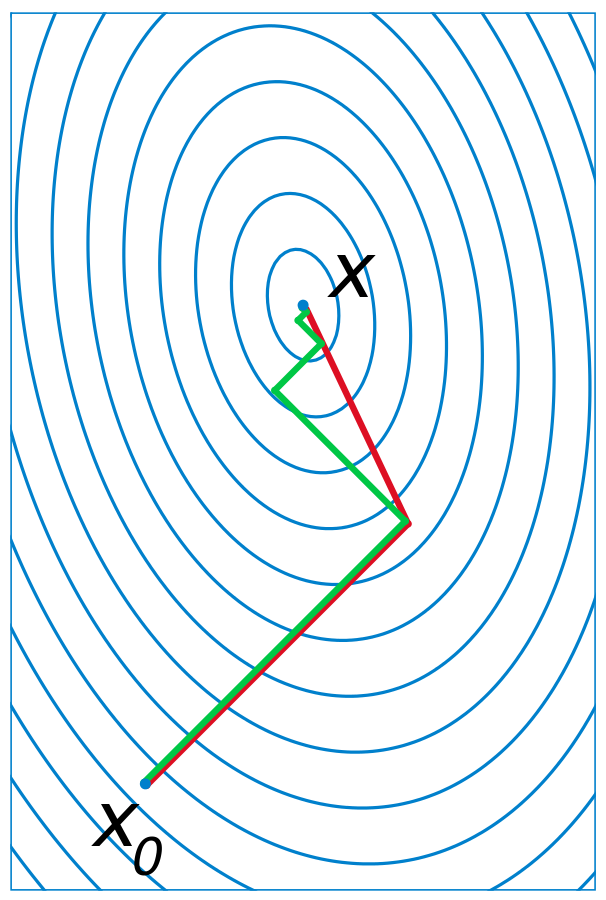
\includegraphics[width=0.3\linewidth]{./pics/ma/konjug.png}
						\caption{Grün: Gradient, Rot: Konjugierter Gradient}
						\label{}
					\end{figure}
					In der Abbildung ist zu erkennen, dass der "`rote"' Weg schneller am gesuchten Ziel X ist als der Grüne. 
				\paragraph{Newton-Verfahren}
					Grundlage für das Quasi-Newton-Verfahren ist das Newton-Verfahren, welches ein Iterationsverfahren ist und auf einen bestimmten Wert konvergiert. Ausgehend von einem Startwert $x_0$ wird anschließend folgende Iteration durchgeführt:
					\[ x_{n+1}= x_n - \frac{f(x_n)}{f'(x_n)}\]
					Dieses Verfahren wird zur Identifikation von Nullstellen verwendet. Um das Verfahren auf ein Optimierungsproblem anzuwenden, wird jedoch das Minimum benötigt. Die Formel ändert sich somit zu:
					\[ x_{n+1}= x_n - \frac{f'(x_n)}{f''(x_n)}\]
					Im mehrdimensionalen entspricht hierbei die erste Ableitung dem Gradienten und die zweite Ableitung der Hesse Matrix. Es ergibt sich somit:
					\[ x_{n+1}= x_n - H^{-1}(x_n)\nabla f(x_n)\]
					Dieses Verfahren hat jedoch einige Nachteile:	
					\begin{enumerate}
						\item Bei jedem Iterationsschritt muss die Hesse Matrix berechnet werden, was sehr aufwendig ist.
						
						\item Bei jedem Iterationsschritt muss die Newtongleichung
						\[d = - H^{-1}(x_n)\nabla f(x_n)\]
						gelöst werden. Wobei d der Suchrichtung entspricht. 
					\end{enumerate}
					
					
				\paragraph{Quasi-Newton-Verfahren}
					Das Quasi-Newton-Verfahren gehört zu den Verfahren, die zur Lösung von nichtlinearen Optimierungsproblemen verwendet werden.
					Um diese Nachteile zu umgehen wurden nun die Quasi-Newton-Verfahren entwickelt. Es wird hierbei zwischen dem direkten und dem inversen Quasi-Newton verfahren unterschieden. Im Folgenden wird nun näher auf das inverse Verfahren eingegangen. Anstelle der inversen Hesse Matrix selbst wird hier nur eine geeignet Approximation $B_n$ verwendet. Es ergibt sich die Gleichung: 
					\[ x_{n+1}= x_n - B(x_n)\nabla f(x_n)\]
					An die Matrix $B$ werden jedoch einige Anforderungen gestellt. 					
					\begin{enumerate}
						\item Die Matrix $B_n$ muss symmetrisch sein, da auch die Hesse-Matrix symmetrisch ist.						
						\item Die Matrix $B_{n+1}$ muss der inversen Quasi-Newton-Gleichung
						\[ B_{n+1} s_n = y_n\]
						genügen. Wobei 
						\[ s_{n}= x_{n+1} - x_n; \qquad y_{n}=\nabla f(x{n+1})-\nabla f(x{n})\]
						entspricht.						
						\item Die Matrix $B_{n+1}$ sollte sich relativ einfach aus $B_n$ berechnen lassen.
					\end{enumerate}					
					Für die Berechnung von $B_{n+1}$ wird hier beispielhaft das Davidon-Fletcher-Powell Verfahren gezeigt. Bei diesem Verfahren berechnet sich $B_{n+1}$ folgendermaßen:
					\[ B_{n+1} = B_n + \frac{s_n {s_n}^T}{{s_n}^T y_n}- \frac{B_n y_n {y_n}^T B_n} {{y_n}^T B_n y_n}\]
					Das Verfahren konvergiert nun, wenn ein bestimmtes Abbruchkriterium erreicht ist. Ein Abbruchkriterium wäre zum Beispiel, dass der Gradient unter einem bestimmten Wert liegt.
				\paragraph{Downhill-Simplex-Verfahren/ Nelder-Mead-Verfahren}
					Das Downhill Simplex Verfahren (auch Nealder Mead Algorithmus genannt) ist ein Ableitungsfreier Suchalgorithmus für lokale Minima bzw. Maxima. Er ist robust gegenüber Unstetigkeiten und besitzt lineare Konvergenz.\\\\
					Simplex bezeichnet das einfachste Volumen in $\mathbb{R}^{n} $ aus $n+1$ Punkten. Beispielsweise ist ein Simplex in $\mathbb{R}^{1} $ eine Strecke oder in $\mathbb{R}^{2} $ ein Dreieck.
					\\\\
					Der Algorithmus ist dabei Folgendermaßen aufgebaut:
					\begin{enumerate}
						\item Wähle $n+1$ Punkte die ein Simplex bilden. 
						\item Sortiere sie nach Wertigkeit $ f(x_{0}) \leq f(x_{1}) \leq . . . \leq f(x_{n}) $.
						\item Berechne den Mittelpunkt $ m = \frac{1}{n}\Sigma_{i=0}^{n-1}x_{i} $ von allen außer den schlechtesten Punkt.
						\item Reflektiere den schlechtesten Punkt $ x_{n} $ am Mittelpunkt $ m $ (reflektierter Punkt $ r = m + \alpha(m-x_{n}) $ wobei $ \alpha $ meist 1 gewählt wird).
						\begin{itemize}
							\item Wenn $ r $ zwischen besten und schlechtesten Wert liegt, ersetze $ x_{n} $ durch $ r $ und gehe zu 3. .
							\item Wenn r bester Wert gehe zu 5. .
							\item Wenn r schlechtester Wert gehe zu 6. .
						\end{itemize}
						\item Expandiere noch weiter in Richtung des Reflektierten Punktes.
						(expandierter Punkt $ e = m + \beta(m-x_{n}) $ wobei $ \beta > \alpha $ ).
						\begin{itemize}
							\item Wenn e besser als r ersetze $ x_{n} $ durch $ e $ und gehe zu 3. .
							\item Wenn e nicht besser oder gleich r, ersetze $ x_{n} $ durch $ r $ und gehe zu 3. .  
						\end{itemize}
						\item Kontrahiere den schlechtesten Punkt $ x_{n} $ (kontrahierter Punkt $ k = m + \gamma(m-x_{n}) $ wobei $ \gamma $ normalerweise $ -\frac{1}{2} $ gewählt wird).
						\begin{itemize}
							\item Wenn k besser als schlechtester Punkt ist, ersetze $ x_{n} $ durch $ k $ und gehe zu 3. . 
							\item sonst gehe zu 7. .
						\end{itemize}
						\item Komprimiere alle außer den besten Punkt $ x_{i} = x_{i} + \delta(x_{i} - x_{0}) $ für $ i = 1,...,n $ und $ \delta < 1 $; danach zu 3. .
					\end{enumerate}
					
					\begin{figure}[h]
						\centering
						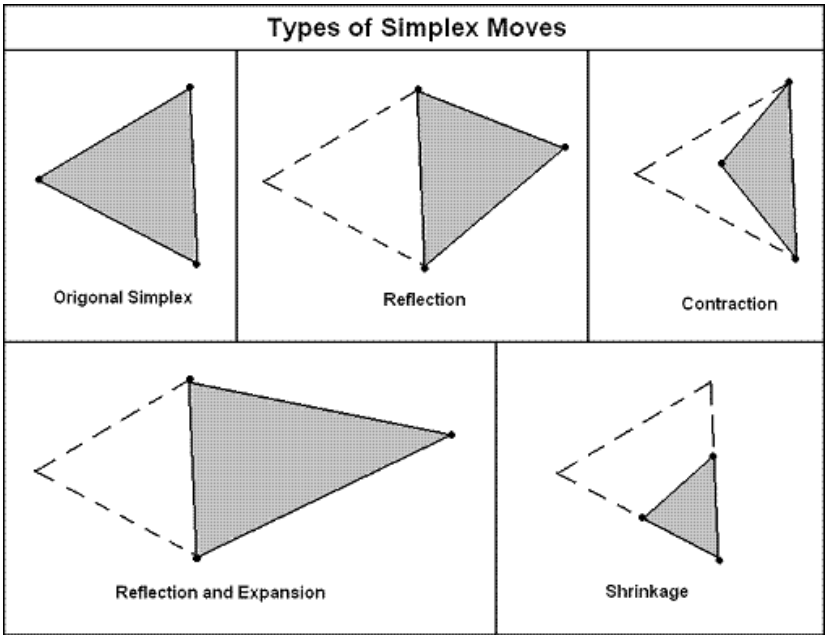
\includegraphics[width=0.5\linewidth]{./pics/ma/DownhillSimpexSchritte}
						\caption{Downhill Simplex Schritte in n = 2}
						\label{fig:DownhillSimpexSchritte}
					\end{figure}
		\subsection{\textcolor{red}{Stochastische Optimierungsverfahen}}
			\subsubsection{\textcolor{red}{Evolutionäre Algorithmen}}
				\paragraph{\textcolor{red}{Genetische Algorithmen}}
				\paragraph{\textcolor{red}{Schwarmintelligenz-Verfahren}}
	Multimodal: Funktion hat mehrere lokale Minimas.
	

	
\section{\textcolor{red}{Numerische Mathematik}}
	\subsection{\textcolor{red}{Lineare Gleichungssysteme - Lösungsverfahren}}
	\subsection{\textcolor{red}{Nichtlineare Gleichungssysteme - Lösungsverfahren}}
	\subsection{\textcolor{red}{Numerische Integration - Lösungsverfahren}}
	\subsection{\textcolor{red}{Numerische Approximation und Interpolation}}
	\subsection{\textcolor{red}{Gewöhnliche Differentialgleichungen - Lösungsverfahren}}
	\subsection{\textcolor{red}{Partielle Differentialgleichungen - Lösungsverfahren}}
	\subsection{\textcolor{red}{Eigenwertberechnung - Lösungsverfahren}}
	\subsection{\textcolor{red}{FFT - schnelle Fourier-Transformation}}


\part{Mechanik}
\section{Begrifflichkeiten}
	\subsection{Generalisierte Koordinaten}
		Die generalisierten (oder verallgemeinerten) Koordinaten bilden in der Theoretischen Mechanik und der Technischen Mechanik einen minimalen Satz von unabhängigen Koordinaten zur eindeutigen Beschreibung des räumlichen Zustands des betrachteten Systems. Sie werden so gewählt, dass die mathematische Formulierung von Bewegungen, die Zwangsbedingungen unterliegen, möglichst einfach wird. Z. B. genügt beim mathematischen Pendel statt der x- und z-Koordinate des Massenpunkts die Angabe des Auslenkwinkels, um die Lage eindeutig zu beschreiben. Die konstante Seillänge ist durch die Bindungsgleichung 
		$ l = const $gegeben.
		\begin{figure}[h]
			\centering
			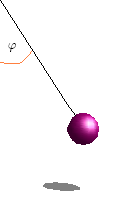
\includegraphics[width=0.15\linewidth]{./pics/me/Pendel}
			\caption{Für das Pendel in der Ebene ergibt sich ein Freiheitsgrad und somit eine generalisierte Koordinate; und zwar $ \phi $}
		\end{figure}
		\leavevmode\\
		Allgemein stimmt die Anzahl der generalisierten Koordinaten, die zur Beschreibung eines Systems mindestens erforderlich sind, mit der Anzahl seiner Freiheitsgrade überein. Die generalisierten Koordinaten spannen den Konfigurationsraum auf.
	\subsection{Arten von Kräften}
		\textbf{Generalisierte Kräfte} sind alle Kräfte die keine Zwangskräfte sind. Sie haben nicht zwangsweise die Einheit der Kraft sondern das Produkt der generalisierte Kraft und zugehöriger generalisierter Koordinate hat die Einheit der Arbeit. So besitzt z.B. die gen. Kraft zu einem Winkel als Koordinate (dimensionslos), die Einheit $ Nm $.\\\\
		\textbf{Zwangskraft} ist beispielsweise die Kraft die vom Untergrund auf einen Klotz wirkt, da er durch die Erdbeschleunigung nach unten gedrückt wird.\\\\
		\textbf{Konservative Kräfte} sind Kräfte die entlang eines geschlossenen Wegintegrals keinerlei Arbeit verrichten. D.h. der Energieinhalt ist am Ende wieder der gleiche. \\\\
		Bei \textbf{Nicht-konservative Kräfte} wird Energie abgeführt (z.B. Reibung). Demnach sind Reibkräfte oder Dämpferkräfte nicht-konservativ. Aber auch Kräfte die Energie in ein System einbringen, wie etwa ein Antriebsdrehmoment sind ebenfalls nicht-konservativ.
	\subsection{Holonome Systeme}
		Ein holonomes System ist in der Mechanik ein System von Körpern, für welches die Lage der Körper über $ n $ generalisierte Koordinaten $ q_{1},q_{2},...,q_{n} $ beschrieben werden kann. Die Koordinaten können entweder vollständig unabhängig voneinander oder über $ m<n $ Zwangsbedingungen miteinander verknüpft sein. 
		\[dim(\bm{q})=dim(DOF)\]
		
		
\section{\textcolor{red}{Kinematik}}
\section{\textcolor{red}{Kinetik}}
\part{Elektrotechnik}
	\section{Grundlagen}
		\subsection{Maxwell-Gleichungen}
			\subsubsection{Mikroskopisch}
				Die mikroskopischen Maxwell-Gleichungen verknüpfen die elektrische Feldstärke $ \bm{E} $ und die magnetische Flussdichte $ \bm{B} $ mit der Ladungsdichte $ \bm{\rho} $  (Ladung pro Volumen) und der elektrischen Stromdichte $ \bm{S} $ (Strom pro durchflossene Fläche).
				\begin{enumerate}
					\item \textbf{Maxwell'sche Gleichung - Durchflutungsgesetz}
					\begin{tcolorbox}[leftrule=3mm]
						 \begin{equation}
						 \text{rot} \bm{B} = \mu_{0}\bm{S} +  \mu_{0}\varepsilon_{0}\frac{\partial\bm{E}}{\partial t}
						 \end{equation}	
					\end{tcolorbox}
					Während sich ein elektrisches Feld ändert, ist es von ringförmigen geschlossenen magnetischen Feldlinien umgeben.
						 
					\item \textbf{Maxwell'sche Gleichung - Induktionsgesetz}
					\begin{tcolorbox}[leftrule=3mm]
						\begin{equation}
							\bm{\nabla} \times \bm{E}=\text{rot}(\bm{E})=-\frac{\partial \bm{B}}{\partial t}
						\end{equation}
					\end{tcolorbox}
	
					\item \textbf{Maxwell'sche Gleichung - Quellenfreiheit (Divergenzfreiheit) von magnetischen Feldern}
					\begin{tcolorbox}[leftrule=3mm]
						\begin{equation}
						\bm{\nabla \cdot B} = \text{div}(\bm{B}) = 0
						\end{equation}
					\end{tcolorbox}
					
					\item \textbf{Maxwell'sche Gleichung - Quellenbehaftetes elektrisches Feld (Divergenz)}
					\begin{tcolorbox}[leftrule=3mm]
						\begin{equation}
						\bm{\nabla \cdot E} = \text{div}(\bm{E}) = \frac{\rho}{\varepsilon_{0}}
						\end{equation}
					\end{tcolorbox}
				\end{enumerate}
			\subsubsection{Makroskopisch}
				Bei Anwesenheit von Materie sind die mikroskopischen Maxwell-Gleichungen einerseits unhandlich, da schließlich jeder Ladungsträger in jedem Atom des Mediums berücksichtigt werden muss. Andererseits können die magnetischen Eigenschaften (beispielsweise von einem Permanentmagneten) prinzipiell nicht ohne zusätzliche physikalische Erkenntnisse der Quantenmechanik aus den mikroskopischen Maxwell-Gleichungen abgeleitet werden. Die makroskopischen Maxwell-Gleichungen berücksichtigen die Eigenschaften der Materie in Form von Materialparametern, wobei dem leeren Raum die Parameter Permittivität $ \varepsilon_{0} $ und Permeabilität $ \mu_{0} $ zugeordnet werden. \\
				Die Anwesenheit von Materie erfordert, dass das elektrische und das magnetische Feld jeweils durch zwei zusätzliche Vektorfelder beschrieben werden, der elektrischen Flussdichte $ \bm{D} := \varepsilon_{0}\bm{E} + \bm{P} $ und der magnetischen Feldstärke $ \bm{H} := \frac{1}{\mu_{0}}\bm{B} - \bm{M} $. Dabei wird $ \bm{P} $ als Polarisation und $ \bm{M} $ als Magnetisierung bezeichnet.\\
				\begin{tcolorbox}[title=Erste Maxwell'sche Gleichung - Durchflutungsgesetz]
					\begin{equation}
						\bm{\nabla} \times \bm{H} = \text{rot} (\bm{H}) = \bm{S} +  \frac{\partial\bm{D}}{\partial t} \quad	\text{bzw.}	 \quad \oint_{S} \bm{H}\cdot d\bm{s} = \int_{A}\bigg(\bm{S} + \frac{d\bm{D}}{dt}\bigg) d\bm{A}		
					\end{equation}
					\tcblower
					Elektrische Ströme, einschließlich Verschiebungsströme führen zu einem magnetischen Wirbelfeld.		
				\end{tcolorbox}	
				
				\begin{tcolorbox}[title=Zweite Maxwell'sche Gleichung - Induktionsgesetz]
					\begin{equation}
					\bm{\nabla} \times \bm{E}=\text{rot}(\bm{E})=-\frac{\partial \bm{B}}{\partial t} \quad	\text{bzw.}	 \quad \oint_{S} \bm{E}\cdot d\bm{s} = -\frac{d}{dt} \int_{A} \bm{B}\cdot d\bm{A}
					\end{equation}
					\tcblower
					Die zweite Maxwellgleichung besagt, dass jedes zeitlich veränderliche magnetische Feld ein elektrisches Wirbelfeld erzeugt. Die Feldlinien des elektrischen Wirbelfeldes sind geschlossen und umgeben ringförmig die Feldlinien des sich ändernden magnetischen Feldes.  Das negative Vorzeichen ergibt sich aus der Lenzschen Regel.
				\end{tcolorbox}	
						
				\begin{tcolorbox}[title=Dritte Maxwell'sche Gleichung - Quellenfreiheit (Divergenzfreiheit) von magnetischen Feldern]
					\begin{equation}
						\bm{\nabla \cdot B} = \text{div}(\bm{B}) = 0
					\end{equation}
					\tcblower
					Das magnetische Feld ist quellenfrei, es gibt keine magnetischen Monopole. D.h. es gibt keine magnetischen Ladungen. Deshalb sind magnetische Felder immer Wirbelfelder mit geschlossenen Feldlinien.
				\end{tcolorbox}	
					
				\begin{tcolorbox}[title=Vierte Maxwell'sche Gleichung - Quellenbehaftetes elektrisches Feld (Divergenz)]
					\begin{equation}
					\bm{\nabla \cdot D} = \text{div}(\bm{D}) = \rho
					\end{equation}
					\tcblower
					Die Ladung ist Quelle und Senke des elektrischen Feldes. Ein solches elektrisches Feld beginnt an positiven Ladungen und endet an negativen Ladungen.
				\end{tcolorbox}	
		
		\newpage
		\subsection{\textcolor{red}{Polarisation}}
		\subsection{Permittivität - Dielektrizität}
			Die Permittivität $ \varepsilon $ gibt in der Elektrodynamik und Elektrostatik die Durchlässigkeit eines Materials für elektrische Felder an. Die Permittivität setzt sich zusammen aus
			\[\varepsilon = \varepsilon_{0}\varepsilon_{r}. \]
			\leavevmode
			\tab[1cm] \textbf{$ \varepsilon_{0} $} \tab ... \tab elektrische Feldkonstante im Vakuum [$ \frac{As}{Vm} $]; $ \varepsilon_{0}=\frac{1}{\mu_{0}c_{0}^{2}}=8.8514878...\cdot10^{-12}\frac{As}{Vm} $ \\\tab[2.5cm]($ c_{0}$ ... Vakuumlichtgeschwindigkeit, $ \mu_{0} $ ... magnetische Feldkonstante)\\
			\tab[1cm] \textbf{$ \varepsilon_{r} $} \tab ... \tab materialabhängige relative Permittivität [$ \frac{As}{Vm} $]; im Vakuum $ \varepsilon_{r}=1 $\\\\
			Aus der elektrischen Flussdichte $ D $ und der Permittivität $ \varepsilon $ erhält man dann das elektrische Feld abhängig vom gegebenen Material
			\[\bm{E}=\frac{\bm{D}}{\varepsilon}=\frac{\bm{D}}{\varepsilon_{0}\varepsilon_{r}}\]
			Wichtige Werte der relativen Permittivität bei 18$^{\circ}$C und einer Feldfrequenz von 50 Hz:\\
			\begin{center}
				\begin{tabular}{l|l}
					\textbf{Medium} & relative Permittivität $ \varepsilon_{r} $ \\\hline
					Vakuum & 1.0\\
					Wasser & 1.77\\
					Luft & 1.00059\\
					CaTiO$ _{3} $ (Ferroelektrikum) & 150 - 180\\
					Polyethylen (90$^{\circ}$C) & 2.4\\
					Aluminiumoxid (Keramik) & 9
					
				
				\end{tabular}
			\end{center}
			Typische Dielektrikas für Kondensatoren sind Polyethylen, PTFE, Keramik (z.b. Steatit, Aluminiumoxid), Glimmer (Mineralien) oder Luft.
		\subsection{\textcolor{red}{Elektrische Feldstärke und Verschiebungsflussdichte}}
		\subsection{\textcolor{red}{Magnetisierung}}
		\subsection{Magnetische Permeabilität}
			Auch magnetische Leitfähigkeit genannt. Sie dient als Faktor für die Abschwächung/ Verstärkung der magnetischen Flussdichte durch ein Material und ergibt sich als
			\[ \mu = \dfrac{B}{H} \]
			\leavevmode
			\tab[1cm] \textbf{B} \tab ... \tab magnetische Flussdichte [$ \frac{Vs}{m^{2}} $]\\
			\tab[1cm] \textbf{H} \tab ... \tab magnetische Feldstärke [$ \frac{A}{m} $]\\\\
			Die magnetische Permeabilität wird dabei durch eine Naturkonstante skaliert, die sogenannte magnetische Feldkonstante $ \mu_{0} = 4\pi\cdot 10^{-7} Vs/Am $. Sie gibt die magnetische Leitfähigkeit des Vakuums an. Für jedes Material kann die magnetische Permeabilität als Produkt aus der Permeabilitätszahl und der magnetischen Feldkonstante angegeben werden.
			\[ \mu = \mu_{r}\cdot\mu_{0}\]
			\tab[1cm] \textbf{$ \bm{\mu_{r}} $} \tab ... \tab relative magnetische Permeabilität (auch Permeabilitätszahl) [dimensionslos]\\\\
			Die Materialkonstante ist für Paramagnetika $ \mu_{r} > 1 $, Diamagnetika $ \mu_{r} = 1$ und für Ferro-, Ferri und Antiferromagnetika eine komplizierte Funktion von Feldstärke und Vorgeschichte ($ \mu_{r} $ bis $ 10^{5} $).\\\\
			\textbf{Diamagnetika:} Gold, $ CO_{2} $, Kupfer, Wasser, Zink, ... \\
			\textbf{Paramagnetika:} Mangan, Chrom, Natrium, Aluminium, ... Auch alle Ferromagnetika gehören dazu. Bei Stoffen in denen Dipole durch ein äußeres Magnetfeld ausgerichtet werden können und dieses somit verstärken.\\
			\textbf{Ferromagnetika:} Eisen, Cobalt, Nickel, ... \\
			\textbf{Ferrimagnetismus:} Kristallstruktur innerhalb welcher sich die magnetischen Momente der Atome abwechselnd antiparallel ausrichten. Diese heben sich gegenseitig aber nicht wie beim Antiferromagnetismus vollständig auf, sondern eine der beiden Richtungen ist stärker.
		\subsection{\textcolor{red}{Magnetische Flussdichte und Feldstärke}}
				
		\subsection{Verschiebungsstrom}
			Verschiebungsstrom (engl. displacement current) ist eine Bezeichnung aus der Elektrodynamik und stellt die Tatsache dar, dass die zeitliche Änderung eines elektrischen Feldes bzw. der elektrischen Flussdichte ein Teil des totalen elektrischen Stromes ist. Der Begriff wurde von James Clerk Maxwell entwickelt und erweitert das Ampèresche Gesetz um einen zusätzlichen Term.\\\\
			Der gesamte elektrische Strom setzt sich grundsätzlich aus zwei additiven Komponenten zusammen:
			\begin{itemize}
				\item Dem \textbf{Leitungsstrom} $ I_{L} $, welcher durch den Fluss von elektrischen Ladungsträgern wie Elektronen oder Ionen getragen wird. Der Leitungsstrom wird durch das elektrische Feld und den damit auf Ladungsträger ausgeübte mechanische Kräfte verursacht.
				\item Der \textbf{Verschiebungsstrom} $ I_{V} $ wird durch die zeitliche Änderungsrate des elektrischen Flusses bestimmt und ist nicht an die Existenz eines elektrischen Leiters gebunden. Der Verschiebungsstrom ist als ein Teil der Wirkung des elektrischen Feldes zu verstehen und drückt im Prinzip die zeitliche Änderungsrate des elektrischen Flusses aus.
			\end{itemize}
			\[I = I_{L} + I_{V}\]
			Dadurch folgt eine begriffliche Erweiterung des Ampèreschen Gesetzes (Durchflutungsgesetz), welche den gesamten elektrischen Strom in der Form								
			\[I = \int_{A} \bigg(\sigma \vec{E} + \varepsilon \frac{\partial \vec{E}}{\partial t}\bigg) \cdot \mathrm{d}\vec{A}\]
			ausdrückt. Dabei stellt der erste Summand den Leitungsstrom dar, welcher von der elektrischen Feldstärke E ausgelöst wird. Die dabei auftretende Konstante $ \sigma $ stellt einen Ausdruck für die elektrische Leitfähigkeit in jenem Medium dar, in welchem sich der Leitungsstrom ausbreitet. Man nennt solche Medien im Regelfall elektrische Leiter.			
			Der zweite Summand stellt den Verschiebungsstrom mit der zeitlichen Änderungsrate der elektrischen Feldstärke und der dielektrischen Leitfähigkeit $\varepsilon $ dar. Die dielektrische Leitfähigkeit drückt die Eigenschaft eines Mediums zur Leitung des elektrischen Flusses aus. Daher fließt der Verschiebungsstrom vor allem in Materialien mit guter dielektrischer und schlechter elektrischer Leitfähigkeit. Man nennt Materialien mit jenen Stoffkonstanten auch Isolatoren.
			\begin{figure}[h]
				\centering
				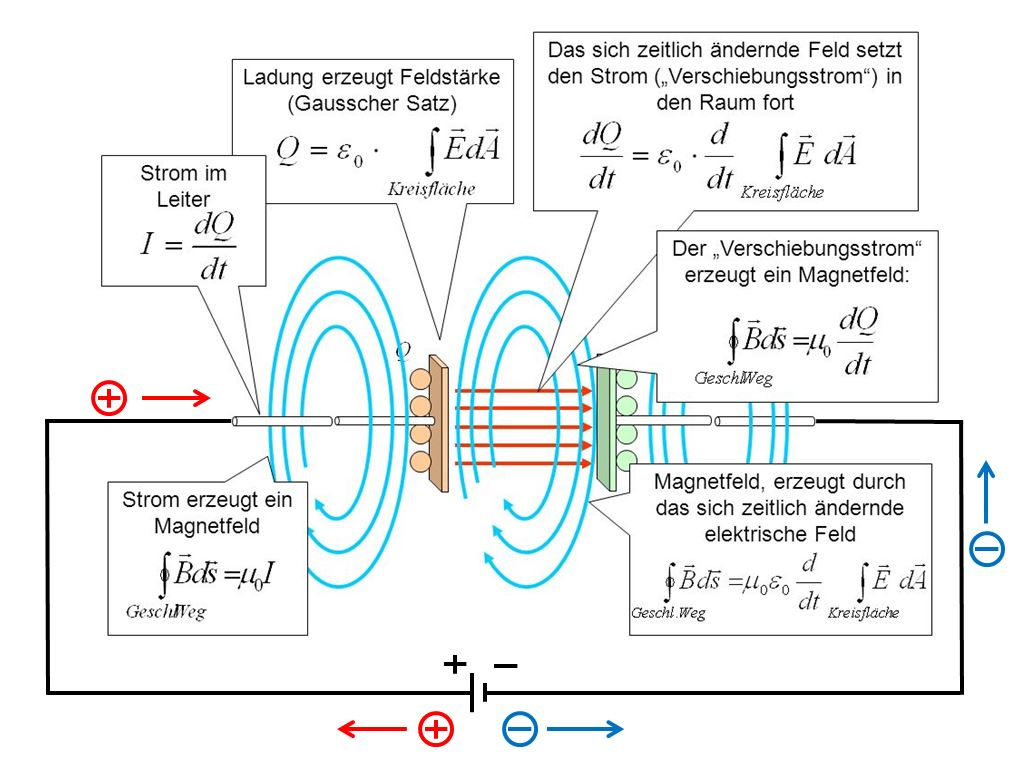
\includegraphics[width=0.8\linewidth]{./pics/el/Iv}
				\caption{Aufladung eines Kondensators als Paradebeispiel für Verschiebungsstrom}
				\label{}
			\end{figure}	
		
		\subsection{Wirbelströme}
			Wie im Induktionsgesetz beschrieben, wird in einem elektrischer Leiter ein Strom induziert wenn sich dieser in einem konstanten Magnetfeld bewegt oder sich in Ruhe in einem sich wechselnden Magnetfeld befindet (= magnetische Flussänderung). Bei einem Draht ist die Stromrichtung eindeutig vorgegeben. Handelt es sich jedoch um einen Leiter mit großer Oberfläche, dann bilden die induzierten Ströme sogenannte Ringströme/Wirbelströme. 
			\begin{figure}[h]
				\centering
				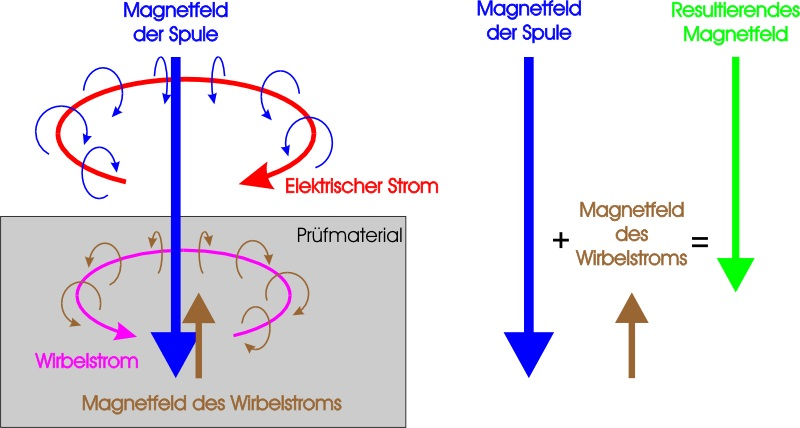
\includegraphics[width=0.7\linewidth]{./pics/el/Wirbel2.jpg}
				\caption{Induktion eines Wirbelstromes}
			\end{figure}
			\leavevmode \\
			Dies ist beispielsweise bei Transformatoren oder Generatoren der Fall. Da Wirbelströme zu Energieverlusten führen, müssen diese durch etwa die Verwendung von Blechpaketen statt einem dicken Eisenkern, reduziert werden. Dabei sind einzelne Bleche elektrisch voneinander isoliert.
		
		\subsubsection*{Wirbelstrombremse}
			Die Wirbelstrombremse ist eine verschleißfreie Bremse. Befindet sich eine Metallplatte in einem inhomogenen Magnetfeld oder wird eine solchige durch ein homogenes Magnetfeld bewegt, werden Wirbelströme induziert. Da die Metallplatte einen ohmschen Widerstand hat, wird die Platte durch die Elektronenbewegung erwärmt. Dies hat zur Folge, dass die Bewegungsenergie der Relativbewegung zwischen Magnetfeld und Metallplatte in Wärmeenergie dissipiert wird. Vorraussetzung für die Induktion von Wirbelströmen, ist das vorhanden sein von freien Ladungsträgern in der Metallplatte (elektrischer Leiter).
			\begin{figure}[h]
				\centering
				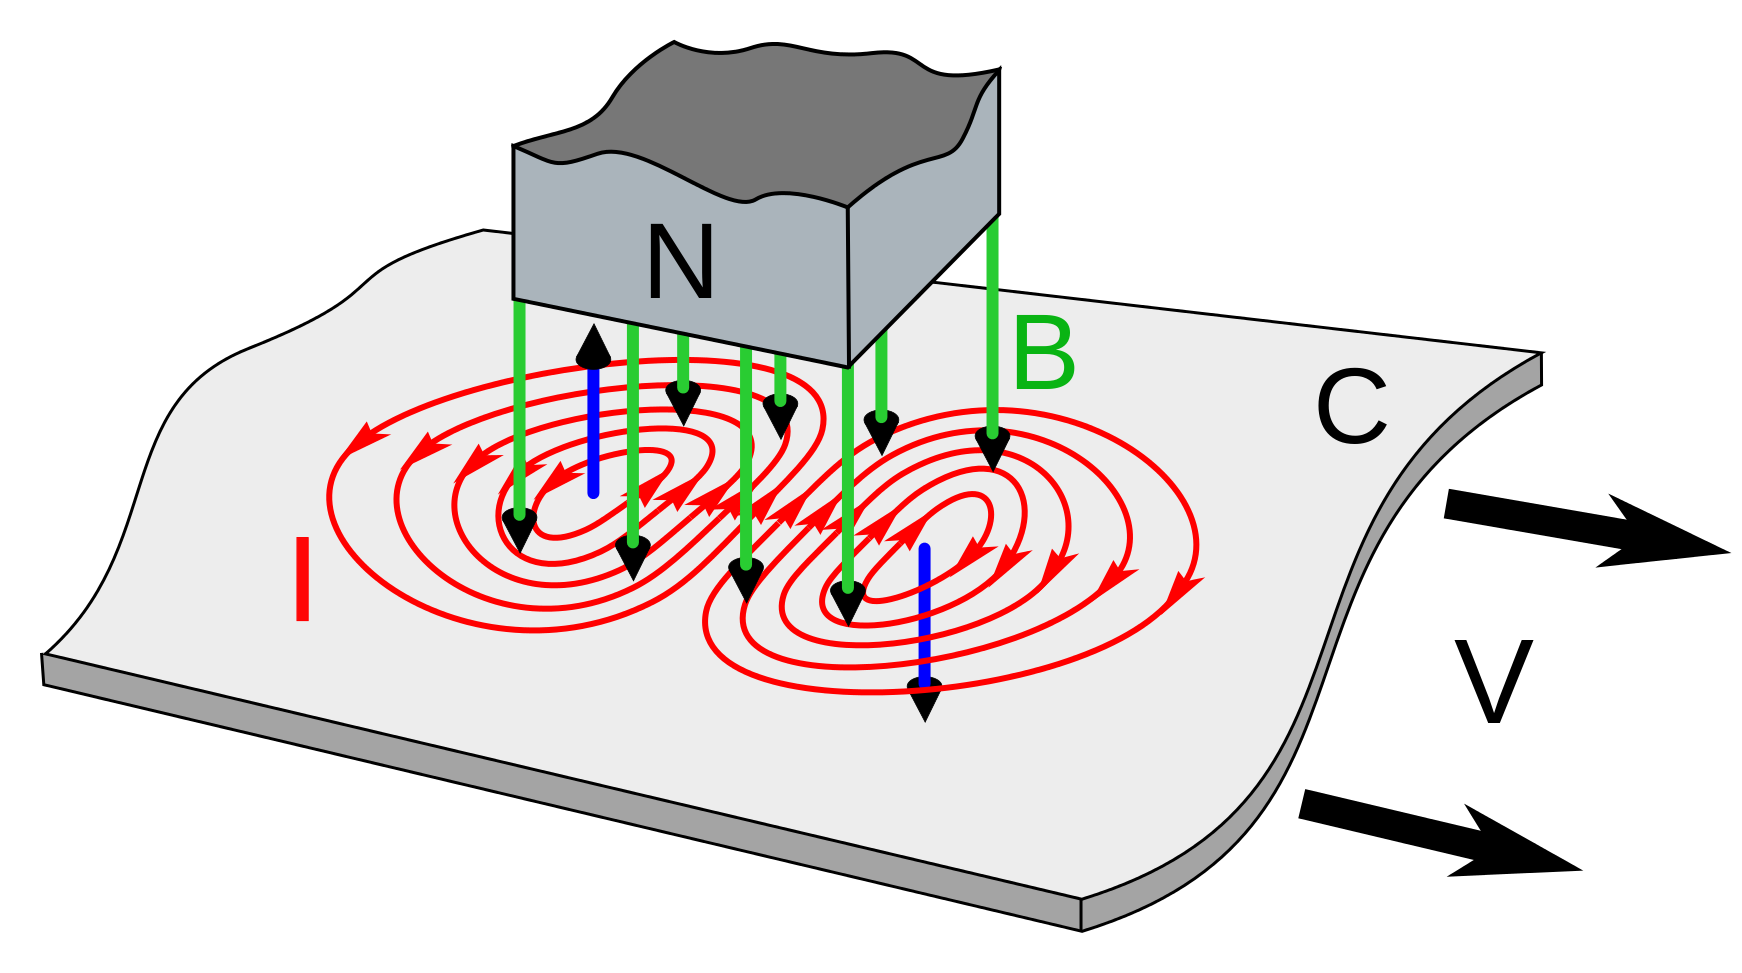
\includegraphics[width=0.49\linewidth]{./pics/el/wirbelbrems1}
				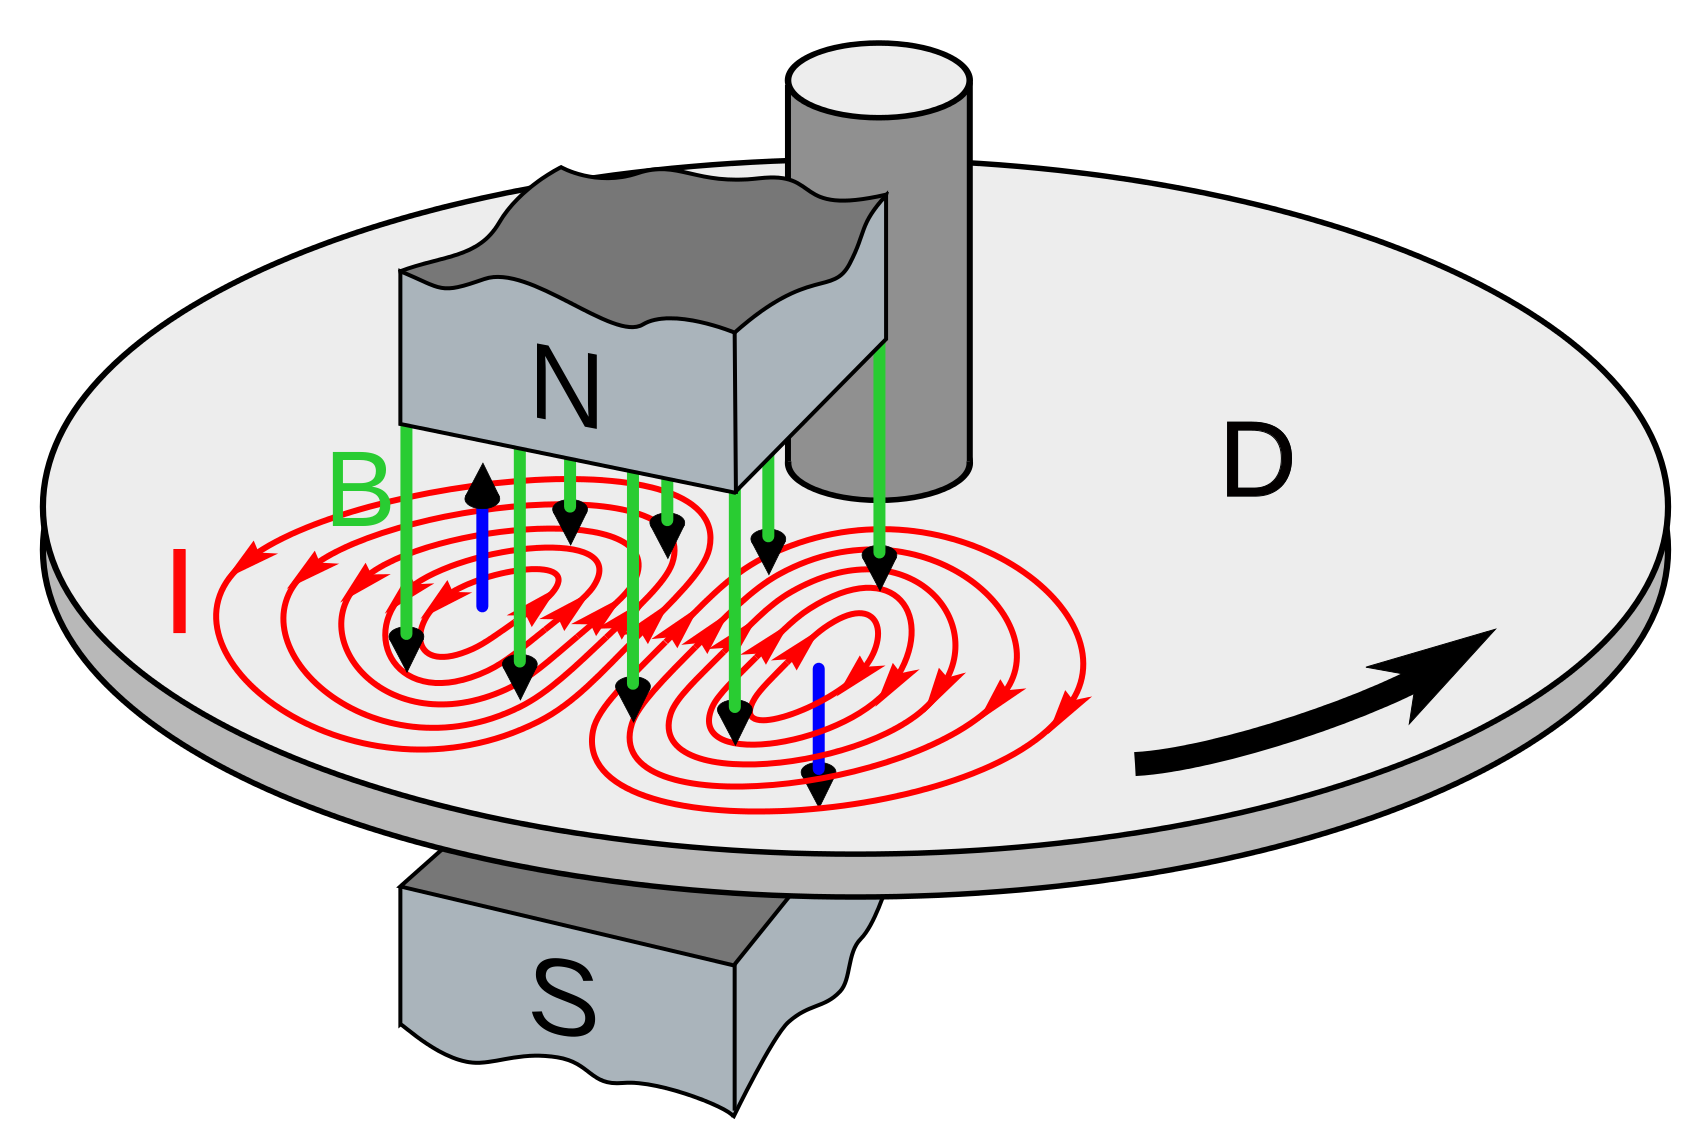
\includegraphics[width=0.49\linewidth]{./pics/el/wirbelbrems2}
				\caption{Beispiele für Wirbelstrombremsen: Zug an Schienen oder LKW an Bremsscheiben}
			\end{figure}
	
		\subsection{Reluktanzkraft/ Maxwellkraft-Prinzip} \label{reluktanzkraft}
			Bei einer stromdurchflossenen Spule, die wie in der Abbildung um einen Eisenkern gewickelt ist, erzeugt die Spule einen magnetischen Fluss im Eisenkern. Es entstehen in beiden Luftspaleten Anziehungskräfte auf den losen Eisenkörper (Anker). Der Effekt der Anziehung beruht darauf, dass die \textit{Reluktanz}, also der magnetishe Widerstand, reduziert und die Induktivität erhöht wird. Das ist der Fall wenn die Feldlinien durch den Anker verlaufen. Wird der Abstand zwischen dem Anker und den Magnetpolen verkürzt, verringert sich der magnetische Widerstand der Feldlinien, denn der Widerstand ist im Eisen wesentlich kleiner als in der Luft.
			\begin{figure}[h]
				\centering
				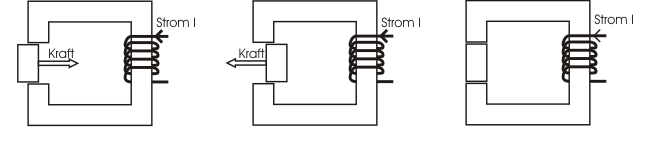
\includegraphics[width=0.7\linewidth]{./pics/el/reluktanz}
			\end{figure}
	
		\subsection{Halbleiter}
			Halbleiter sind Festkörper, deren elektrische Leitfähigkeit zwischen der von elektrischen Leitern und der von Nichtleitern liegt. Da sich die Grenzbereiche der drei Gruppen überschneiden, ist der negative Temperaturkoeffizient des spezifischen Widerstandes ein weiteres wichtiges Merkmal von Halbleitern, das heißt, ihre Leitfähigkeit nimmt mit steigender Temperatur zu, sie sind sogenannte Heißleiter. Ursache hierfür ist die sogenannte Bandlücke zwischen dem Valenz- und dem Leitungsband. Nah am absoluten Temperaturnullpunkt sind diese voll- bzw. unbesetzt und Halbleiter daher Nichtleiter. Es existieren im Gegensatz zu Metallen primär keine freien Ladungsträger, diese müssen erst z. B. durch thermische Anregung entstehen. Die elektrische Leitfähigkeit von Halbleitern steigt aber steil mit der Temperatur an, so dass sie bei Raumtemperatur, je nach materialspezifischem Abstand von Leitungs- und Valenzband, mehr oder weniger leitend sind. Des Weiteren lässt sich durch das Einbringen von Fremdatomen (Dotieren) aus einer anderen chemischen Hauptgruppe die Leitfähigkeit und der Leitungscharakter (Elektronen- und Löcherleitung) in weiten Grenzen gezielt beeinflussen.\\
			Am bekanntesten sind die Elementhalbleiter Silicium und Germanium, die aus einem einzigen Element aufgebaut sind, und Verbindungshalbleitern wie zum Beispiel der III-V-Verbindungshalbleiter Galliumarsenid. Des Weiteren haben in den letzten Jahrzehnten organische Halbleiter an Bedeutung und Bekanntheit gewonnen, sie werden beispielsweise in organischen Leuchtdioden (OLEDs) eingesetzt.
			\begin{itemize}
				\item \textbf{Elementhalbleiter}: Si, Ge, B, Se, Te, C
				\item \textbf{Verbindungshalbleiter}: GaAs, ...
				\item \textbf{Organische Halbleiter}
			\end{itemize}
			\begin{figure}[h]
				\centering
				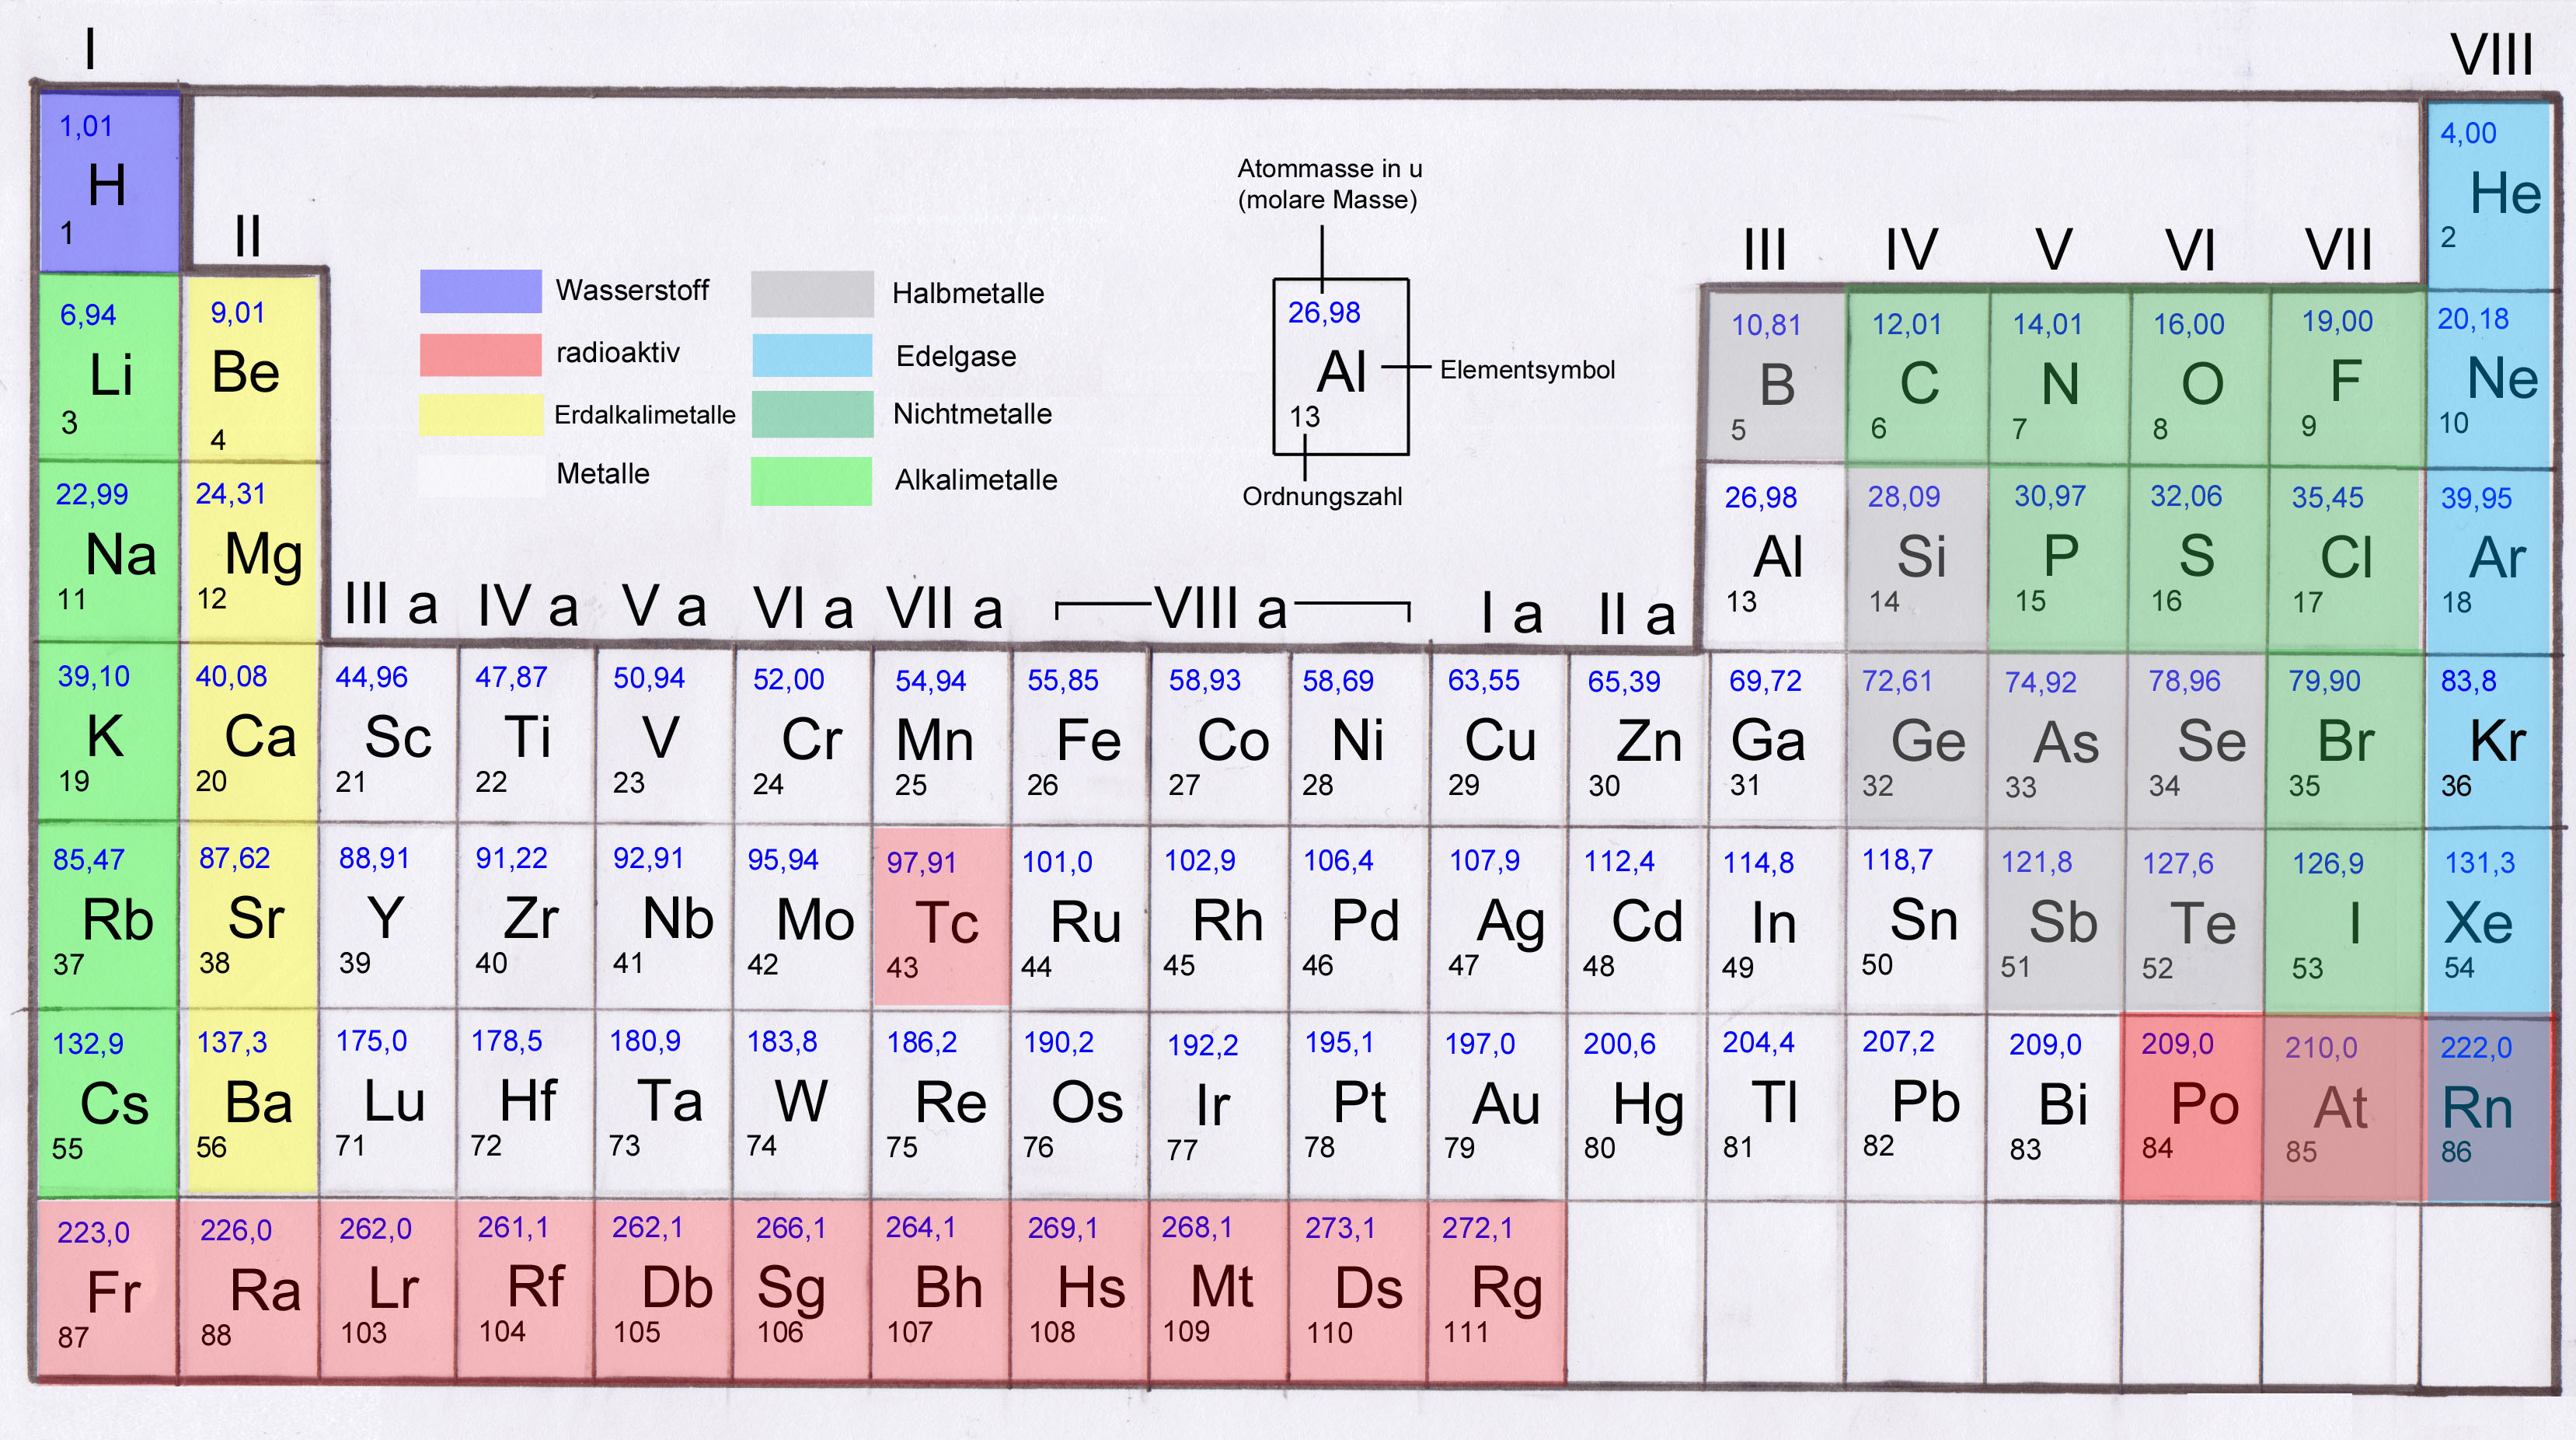
\includegraphics[width=0.73\linewidth]{./pics/el/periodensys}
			\end{figure}

		\subsection{Raumladungszone und p/n-Übergang}
			Für die Herstellung eines Halbleiterbauelements wird der Siliziumkristall verunreinigt. Bei der p-Dotierung werden Fremdatome (Bor) eingefügt die weniger Elektronen als das Silizium besitzen, wodurch sich positive Löcher im Material ausbilden. Bei der n-Dotierung wird Phosphor eingebracht, das mehr Elektronen als das Silizium besitzt und es entsteht ein Material das freie Elektronen besitzt. Dotierte Halbleiter sind in ihrem Grundzustand ungeladen. Es existieren immer gleich viele freie Ladungsträger als ortsfeste Raumladungen der ionisierten Dotierungsatome.
			\begin{figure}[h]
				\centering
				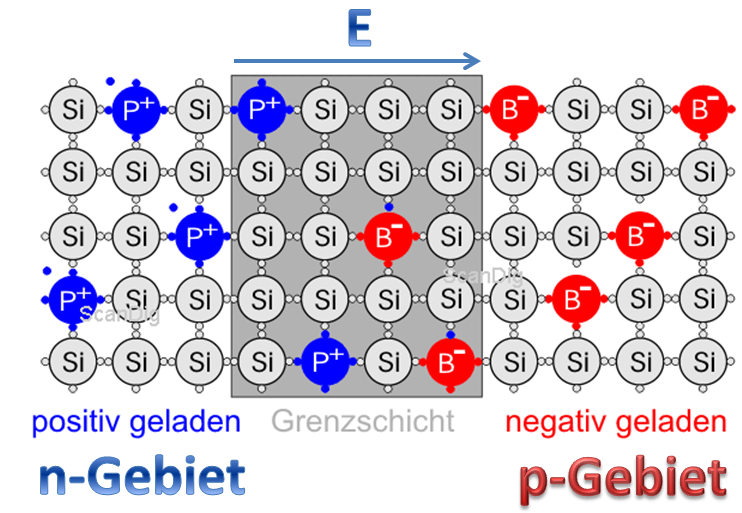
\includegraphics[width=0.4\linewidth]{./pics/el/si}
				\caption{Phosphor mit 5 Protonen im Kern und Bor mit 3 Protonen im Kern, Silizium mit 4 Protonen und Elektronen}
			\end{figure}
			Bringt man diese beiden Materialen aneinander, ergibt sich ein Konzentrationsunterschied von positiven und negativen Ladungsträgern zwischen den beiden Gebieten. Aufgrund von Diffusion streben positive Löcher vom p-dotierten Bereich ins n-Gebiet und negative Elektronen in den p-dotierten Bereich. Positive Löcher rekombinieren im n-Gebiet mit den Elektronen und die Elektronen rekombinieren im p-Gebiet mit den dort vorhandenen Löchern. Es entsteht eine Zone ohne freie Ladungsträger, aber mit positiven Phosphor-Ionen und negativen Bor-Ionen. In weiterer Folge bildet sich ein elektrisches Feld in der Raumladungszone aus. Ist das elektrische Feld groß genug (~0.7V), können die Elektronen des n-Gebiets die Schicht an negativen Bor-Ionen nicht mehr durchdringen und werden von diesen abgestoßen. Das elektrische Feld wirkt der Diffusion entgegen und es hat sich ein Gleichgewicht ausgebildet.
			\subparagraph*{Extern angelegte Spannung} 
				In Durchlassrichtung wirkt das elektrische Feld der externen Spannung, dem elektrischen Feld in der Raumladungszone entgegen. Die positiven Löcher werden vom positiven Pol abgestoßen und die Elektronen vom negativen Pol. Dadurch bewegen sich Elektronen und Löcher zur Mitte Richtung Grenzschicht hin und rekombinieren dort fortlaufend. Ein elektrischer Stromfluss ist möglich. Bei Sperrrichtung liegt genau der umgekehrte Fall vor und die Raumladungszone wird dabei vergrößert.
				\begin{figure}[h]
					\centering
					\subfigure[Durchlassrichtung]
					{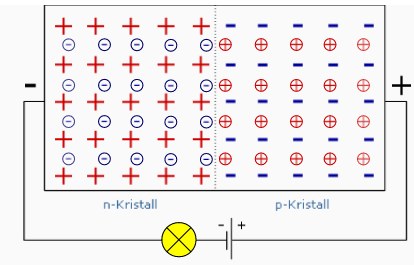
\includegraphics[width=0.35\textwidth]{./pics/el/durchlass}} \hspace{0.4cm}
					\subfigure[Sperrrichtung] 
					{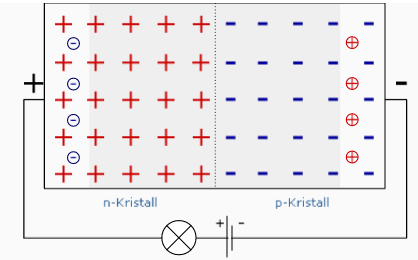
\includegraphics[width=0.35\textwidth]{./pics/el/sperr}}
				\end{figure}

		
	
	\newpage
	\section{Elektrische Bauelemente}
		\subsection{Bipolar-Transistor}
			\subsubsection*{Funktionsweise}
				Im Folgenden wird die physikalische Stromrichtung (Elektronenstrom) für die Erläuterung verwendet. Durch das Anlegen einer Spannung $ U_{BE} $ von etwa 0,7 V, ist die untere Diode (Prinzip) in Durchlassrichtung geschaltet. Die Elektronen gelangen in die p-Schicht und werden von dem Plus-Pol der Spannung $ U_{BE} $ angezogen.
				Da die p-Schicht sehr klein ist, wird nur ein geringer Teil der Elektronen angezogen.
				Der größte Teil der Elektronen bewegt sich weiter in die obere Grenzschicht. Dadurch wird diese leitend und der Plus-Pol der Spannung $ U_{CE} $ zieht die Elektronen an. Es fließt ein Kollektorstrom $ I_{C} $.
				Bei üblichen Transistoren gelangen etwa 99\% der Elektronen von Emitter zum Kollektor durch. In der Basisschicht rekombinieren etwa 1\% der Elektronen.
				\begin{figure}[h]
					\centering
					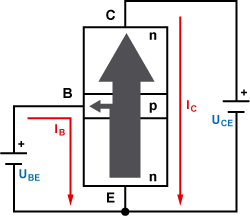
\includegraphics[width=0.4\linewidth]{./pics/el/npn.png}
				\end{figure}
			
	\section{\textcolor{red}{Elektronische Grundschaltungen}}
		\subsection{\textcolor{red}{Wechselrichter}}
			\begin{figure}[h]
				\centering
				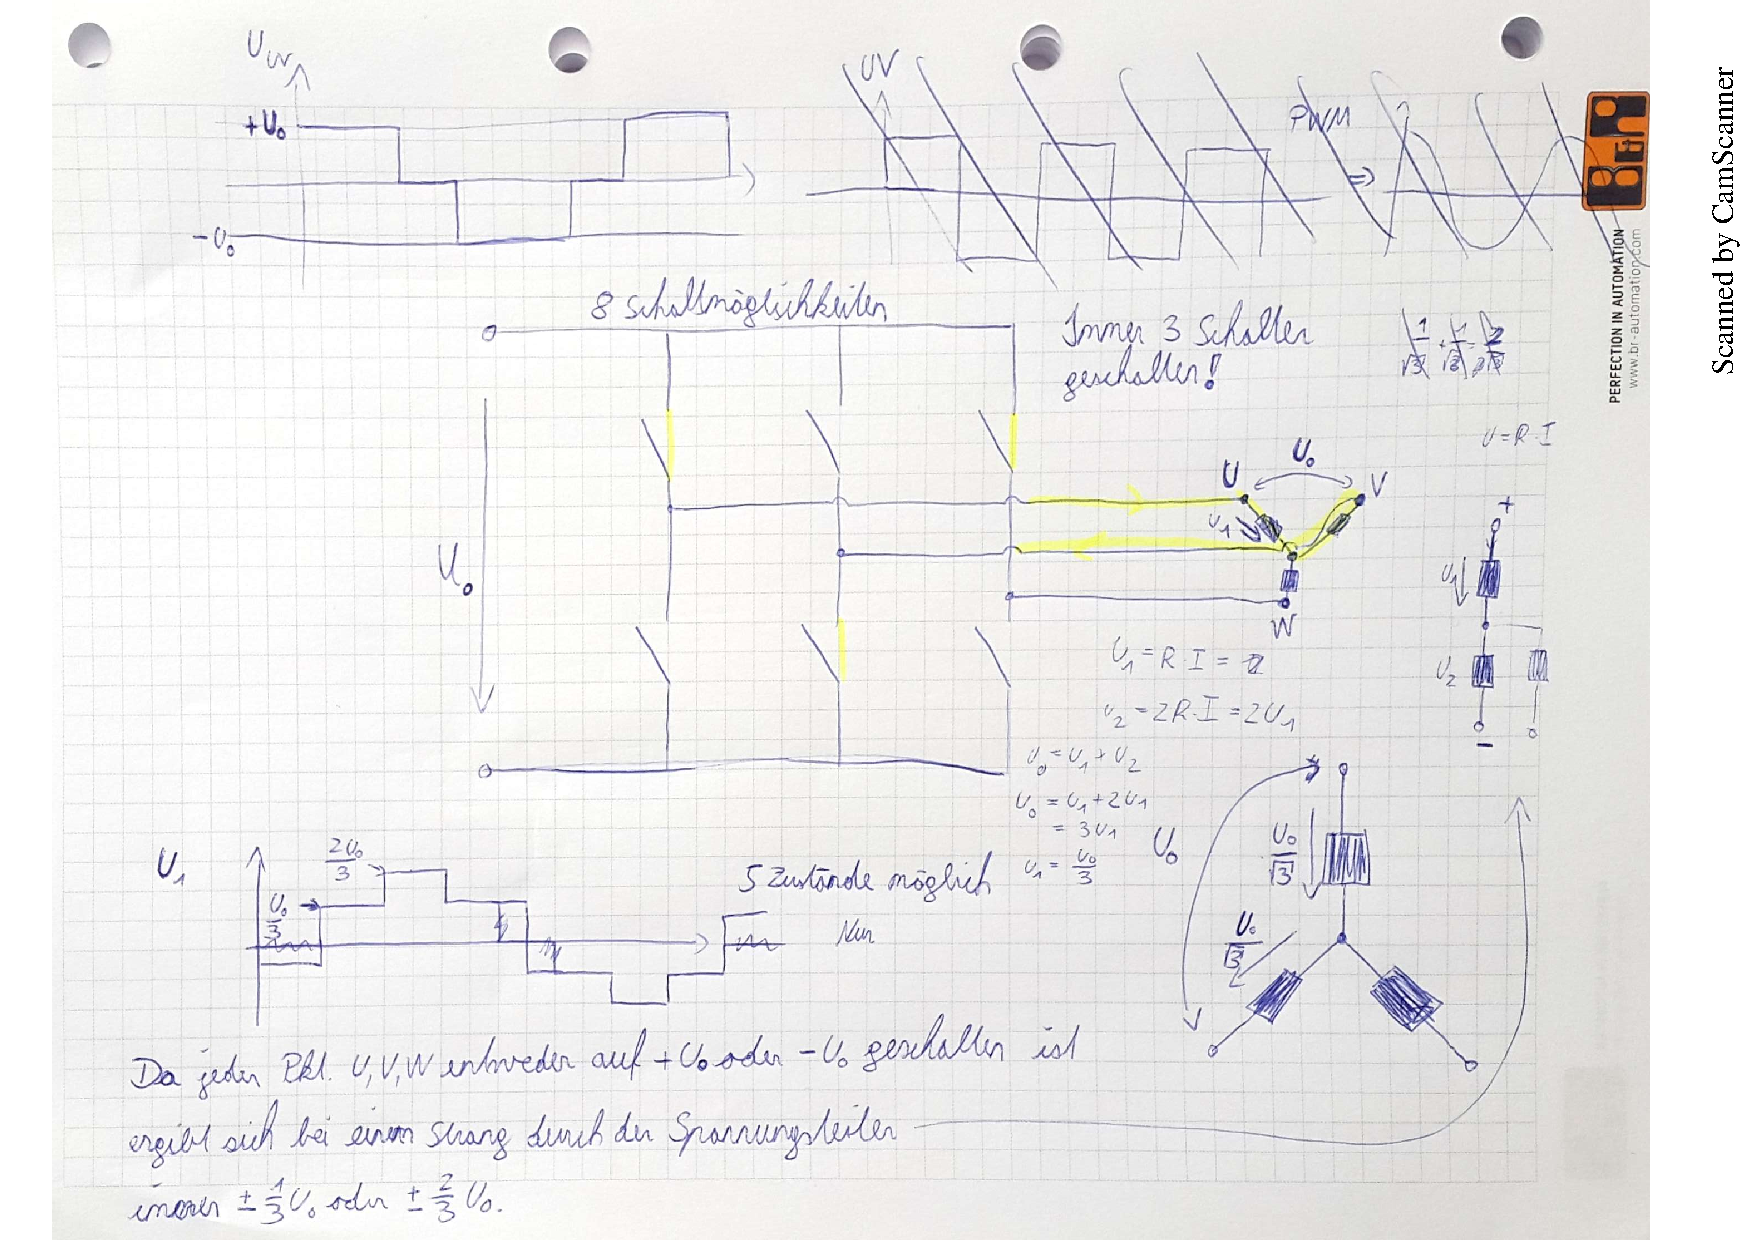
\includegraphics[width=1\linewidth]{./pics/el/wechsel.pdf}
				\caption{}
				\label{}
			\end{figure}
			\begin{figure}[h]
				\centering
				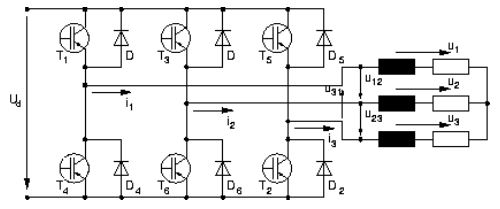
\includegraphics[width=0.5\linewidth]{./pics/el/wechsel1}
				\caption{}
				\label{}
			\end{figure}
			\begin{figure}[h]
				\centering
				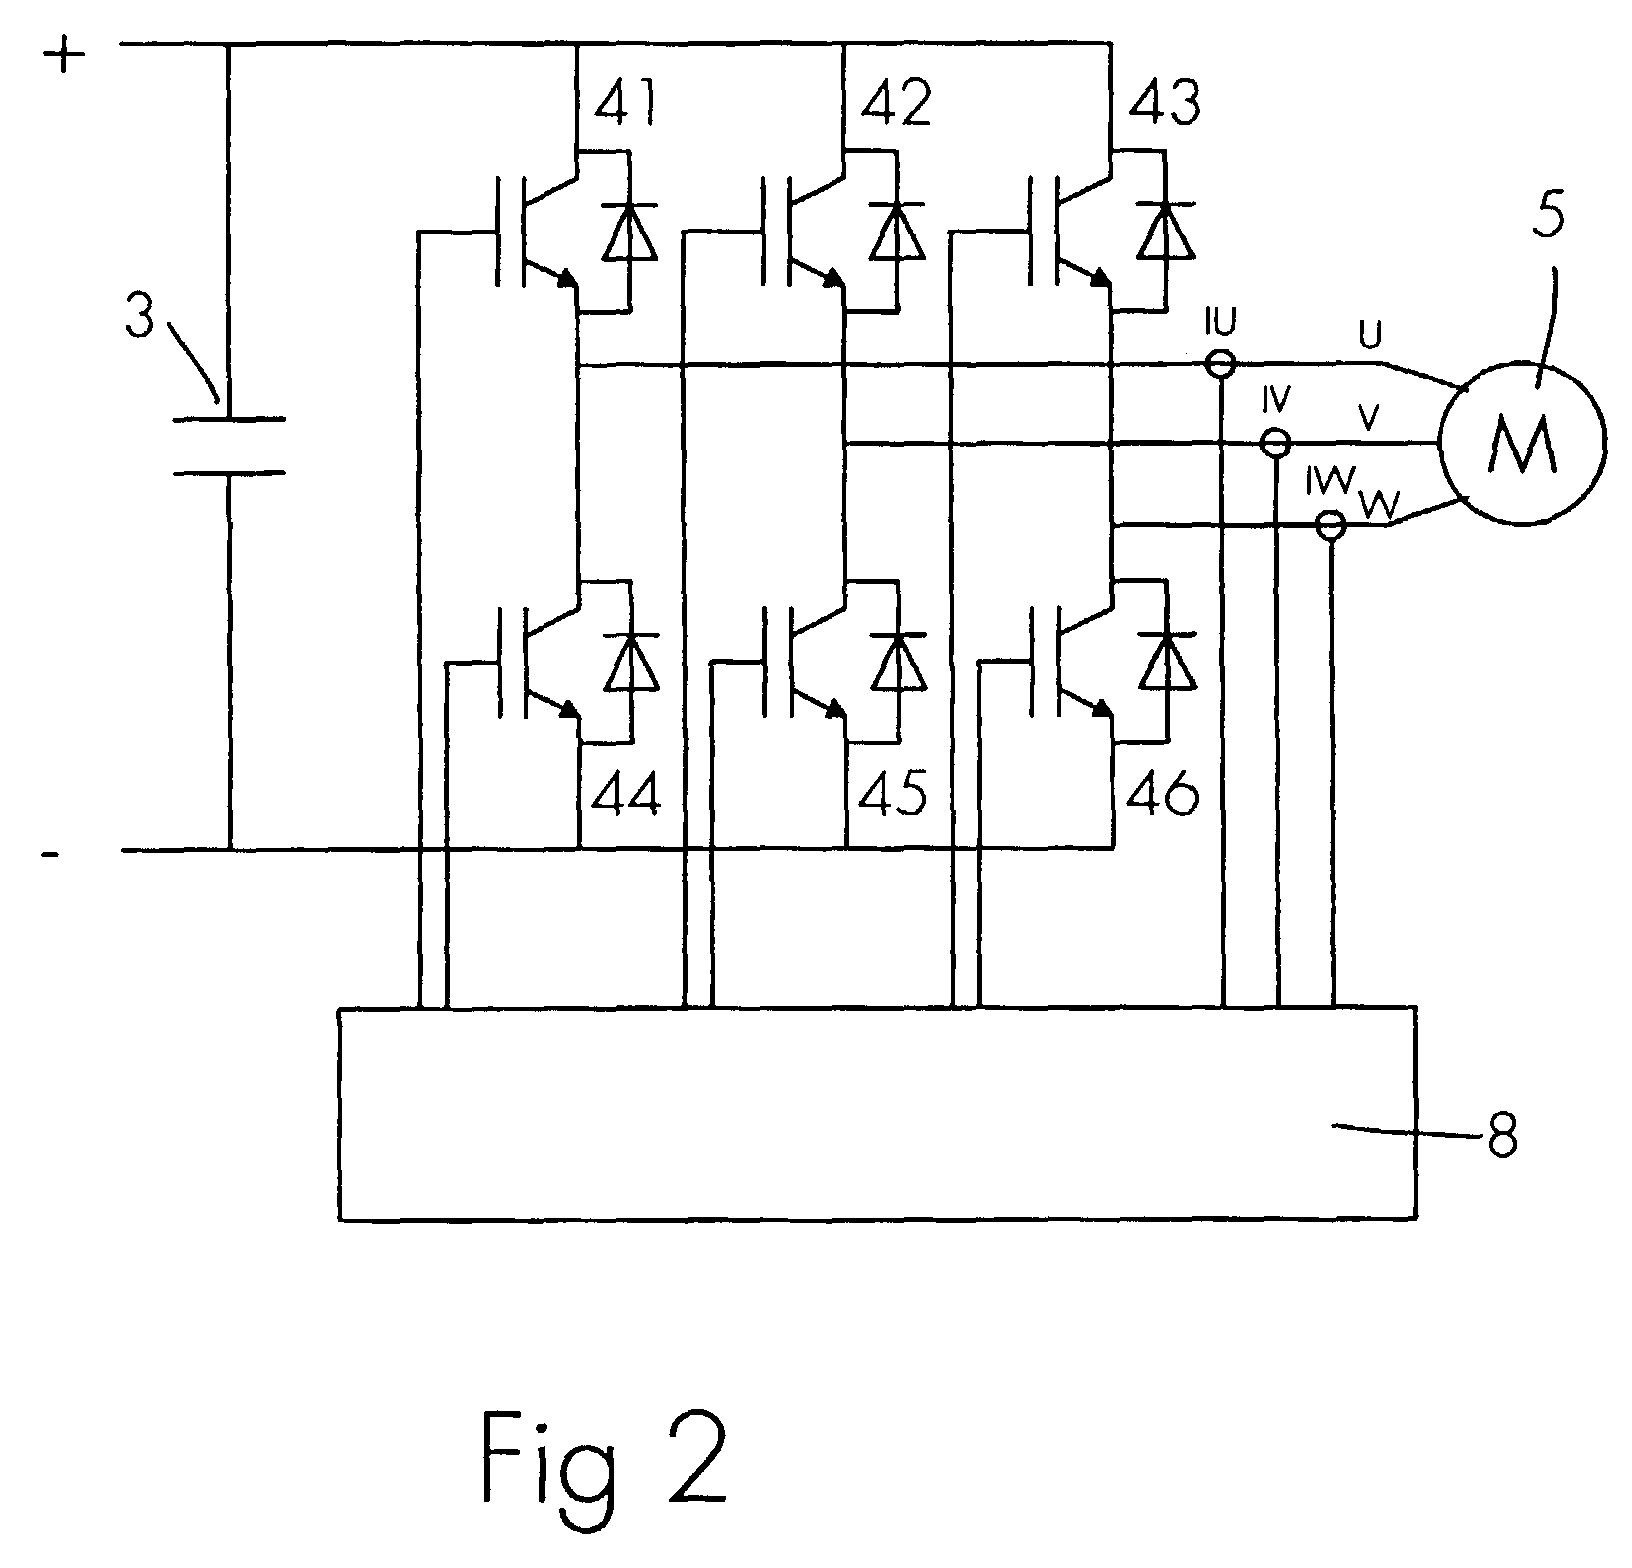
\includegraphics[width=0.5\linewidth]{./pics/el/wechsel2}
				\caption{}
				\label{}
			\end{figure}
			\leavevmode \\
	\section{\textcolor{red}{Filter}}
		\subsection{Filtertypen}
		\begin{itemize}
			\item Tiefpassfilter
			\item Hochpassfilter
			\item Bandpassfilter
			\item Bandsperre, Kerbfilter
			\item Allpassfilter – lässt alle Frequenzen mit gleicher Verstärkung durch, kann aber eine Phasenverschiebung verursachen.
		\end{itemize}
		Die Filterordnung beschreibt die Dämpfung von Frequenzen unterhalb od. oberhalb der Grenzfrequenz. Z.b. bei einem Filter n. Ordnung würde die TF mit $ n\cdot6dB/Oktave $ fallen.\\\\
		Weitere Einteilungen: Aktiv, Passiv, Linear, Nicht-Linear, Ordnung
		\subsection{\textcolor{red}{Analoges aktives Filter}}
		\subsection{\textcolor{red}{Analoges passives Filter}}
			\subsubsection{\textcolor{red}{Topologien}}
			https://de.wikipedia.org/wiki/Analogfilter\\
			http://elektroniktutor.de/analogtechnik/filter.html
			\subsubsection{\textcolor{red}{Tiefpassfilter}}
				Praktische Anwendung, wie wird ein Tiefpassfilter dimensioniert --> gewünschte Grenzfrequenz einstellen
			\subsubsection{\textcolor{red}{Hochpassfilter}}
			\subsubsection{Notchfilter}
				Ein Kerbfilter ist ein elektronisches Filter, mit dem Frequenzen innerhalb eines engen Frequenzbereiches ausgefiltert werden können. Anschaulich wird eine Kerbe in das Frequenzdiagramm eingefügt.
				Kerbfilter stellen einen besonders schmalbandigen Typ von Bandsperrfilter dar, welche in der Übertragungsfunktion nur eine Nullstelle aufweisen und damit nicht ein breites Frequenzband, sondern idealerweise genau eine Frequenz möglichst stark dämpfen.
				
		\subsection{\textcolor{red}{Digitales Filter}}
			\subsubsection{\textcolor{red}{FIR - Finite Impulse Response}}
			\subsubsection{\textcolor{red}{IIR - Infinite Impulse Response}	}		
		\subsection{Kalmanfilter}
			Ein Kalman-Filter schätzt den Wert einer ungenauen oder unsicheren Messung anhand der vorhergegangen Messwerte ab. Das Prinzip beruht auf Wahrscheinlichkeitsfunktionen. Systemzustände müssen dafür bekannt sein und fließen in die Berechnung mit ein. Anders formuliert wird eine Vorhersage des nächsten Wertes anhand des momentanen Wertes und der bekannten System-Eingangsvariablen geschätzt. Zusätzlich vergrößern die nicht abschätzbaren Parameter den Wahrscheinlichkeitsbereich, wo der nächste Wert landen könnte. Hinzu kommt nun noch eine Wahrscheinlichkeit für den Messwert des Sensors. Aufgrund von Rauschen erhalten wir einen anderen Wert als real vorhanden ist. Diese Abweichung wird wiederum als Wahrscheinlichkeit beschrieben. Nun kann man die beiden Wahrscheinlichkeiten (die des nächsten Wertes und der Korrektheit des Messwertes) multiplizieren und erhält einen neuen verbesserten Schätzwert.\\
			Dieser verbesserte Schätzwert kann nun wieder durch den ganzen Ablauf verwendet werden und wir erhalten einen neuen Schätzwert. Dieser Vorgang kann beliebig oft vorgenommen werden.
			Die Filter sind sehr schnell – Echtzeitfähig – und liefern in der Praxis sehr gute Ergebnisse. Zeigt sehr gute Filtereigenschaften für Sensorrauschen (Unsicherheit der Messung ausgleichen).\\
			http://www.bzarg.com/p/how-a-kalman-filter-works-in-pictures/
			
	\section{\textcolor{red}{Sensoren}}
		\subsection{\textcolor{red}{Übersicht von Sensoren nach deren Messgrößen}}
		Abstands- bzw. Wegsensoren
		Geschwindigkeits und Drehzahlsensoren
		Beschleunigungssensoren
		\subsection{Encoder}
			\subsubsection{TTL-Encoder}
				2 Signale A,B mit insgesamt 4 verschiedenen Zuständen --> Drehencoder mit 1000 ppr = 4000 Zustände pro Umdrehung.
			\subsubsection{SinCos-Encoder}
		\subsection{\textcolor{red}{Piezoelektrische Sensoren}}
		\subsection{\textcolor{red}{Induktive Sensoren}}
		\subsection{\textcolor{red}{Kapazitive Sensoren}}
		\subsection{\textcolor{red}{Mechanische Sensoren}}
		\subsection{\textcolor{red}{Thermoelektrische Sensoren}}
		\subsection{\textcolor{red}{Resistive Sensoren}}
		\subsection{\textcolor{red}{Magnetische Sensoren}}
		\subsection{\textcolor{red}{Optische Sensoren}}
			\subsubsection{Interferometer}
				Das Messprinzip basiert auf der Überlagerung von zwei Wellen die unterschiedliche Wege zurücklegen. Grundsätzlich lässt sich mit jeder Art von Welle, seien es elektromagnetische Wellen, Schall- oder Materiewellen, eine Interferenz erzeugen.\\ Laserlicht eignet sich ausgezeichnet für kürzere (Meterbereich) und äußerst präzise (Pikometerbereich) Wegmessungen. Voraussetzung für eine erfolgreiche Interferenz ist, dass Wellen kohärent überlagert werden. Deshalb wird Laserlicht verwendet, da ausgesendete Lichtwellen nahezu phasengleich zueinander sind und eine sehr große Kohärenzlänge (max. Weglänge zweier Lichtstrahlen, bei der diese noch ein stabiles Interferenzmuster ergeben) - d.h. auch über große Distanzen phasengleich bleiben - besitzen. \\
				Die unterschiedlichen Typen von Interferometern haben meist das selbe Funktionsprinzip. Durch Überlagerung zweier Wellen, die in getrennten optischen Bahnen geführt und von Spiegeln bzw. einem Objekt reflektiert werden, bilden ein Interferenzmuster (Interferenzstreifen oder -ringe). Dieses ist abhängig von der Distanz des Objektes. Somit können Distanzänderungen detektiert werden.\\
				So werden beim \textbf{Michelson-Interferometer} durch einen Photosensor abwechselnd Minima und Maxima des Interferenzbildes registriert und mitgezählt. Wird die Anzahl der gemessenen Maxima mit der Wellenlänge des Laserlichts multipliziert, erhält man die Wegdifferenz. Da das Medium durch das die elektromagnetische Welle wandert, deren Wellenlänge beeinflusst, ist ein wichtiger Faktor, die Eigenschaften dieses Mediums zu berücksichtigen (Luftdruck, Luftfeuchtigkeit, Temperatur).\\
				Bei Vielstrahlinterferometern wie dem \textbf{Fabry-Per\'{o}t-Interferometer} wird die Längenänderung gemessen indem die Länge des optischen Resonators verändert wird. D.h. ein optischer Ausgang/Messkopf des Interferometers und das Objekt bilden gemeinsam einen optischen Resonator. Martin Zech von Attocube hat ein solches Interferometer entwickelt, das Genauigkeiten im sub-Nanometerbereich bei Raumtemperatur erreicht. Wird der Sensor mit flüssigem Helium auf 4 K gekühlt kann durch Rauschunterdrückung eine Genauigkeit von 1 pm erreicht werden.\\
		
				Vorteil:
				\begin{itemize}
					\item Höhere Empfindlichkeit 
					\item Längenmessungen bis 10$ ^{-12} $ m Genauigkeit können gemessen werden
				\end{itemize}
		
		
		

	\section{Elektrische Maschinen}
		\leavevmode
		\begin{figure}[h]
			\centering
			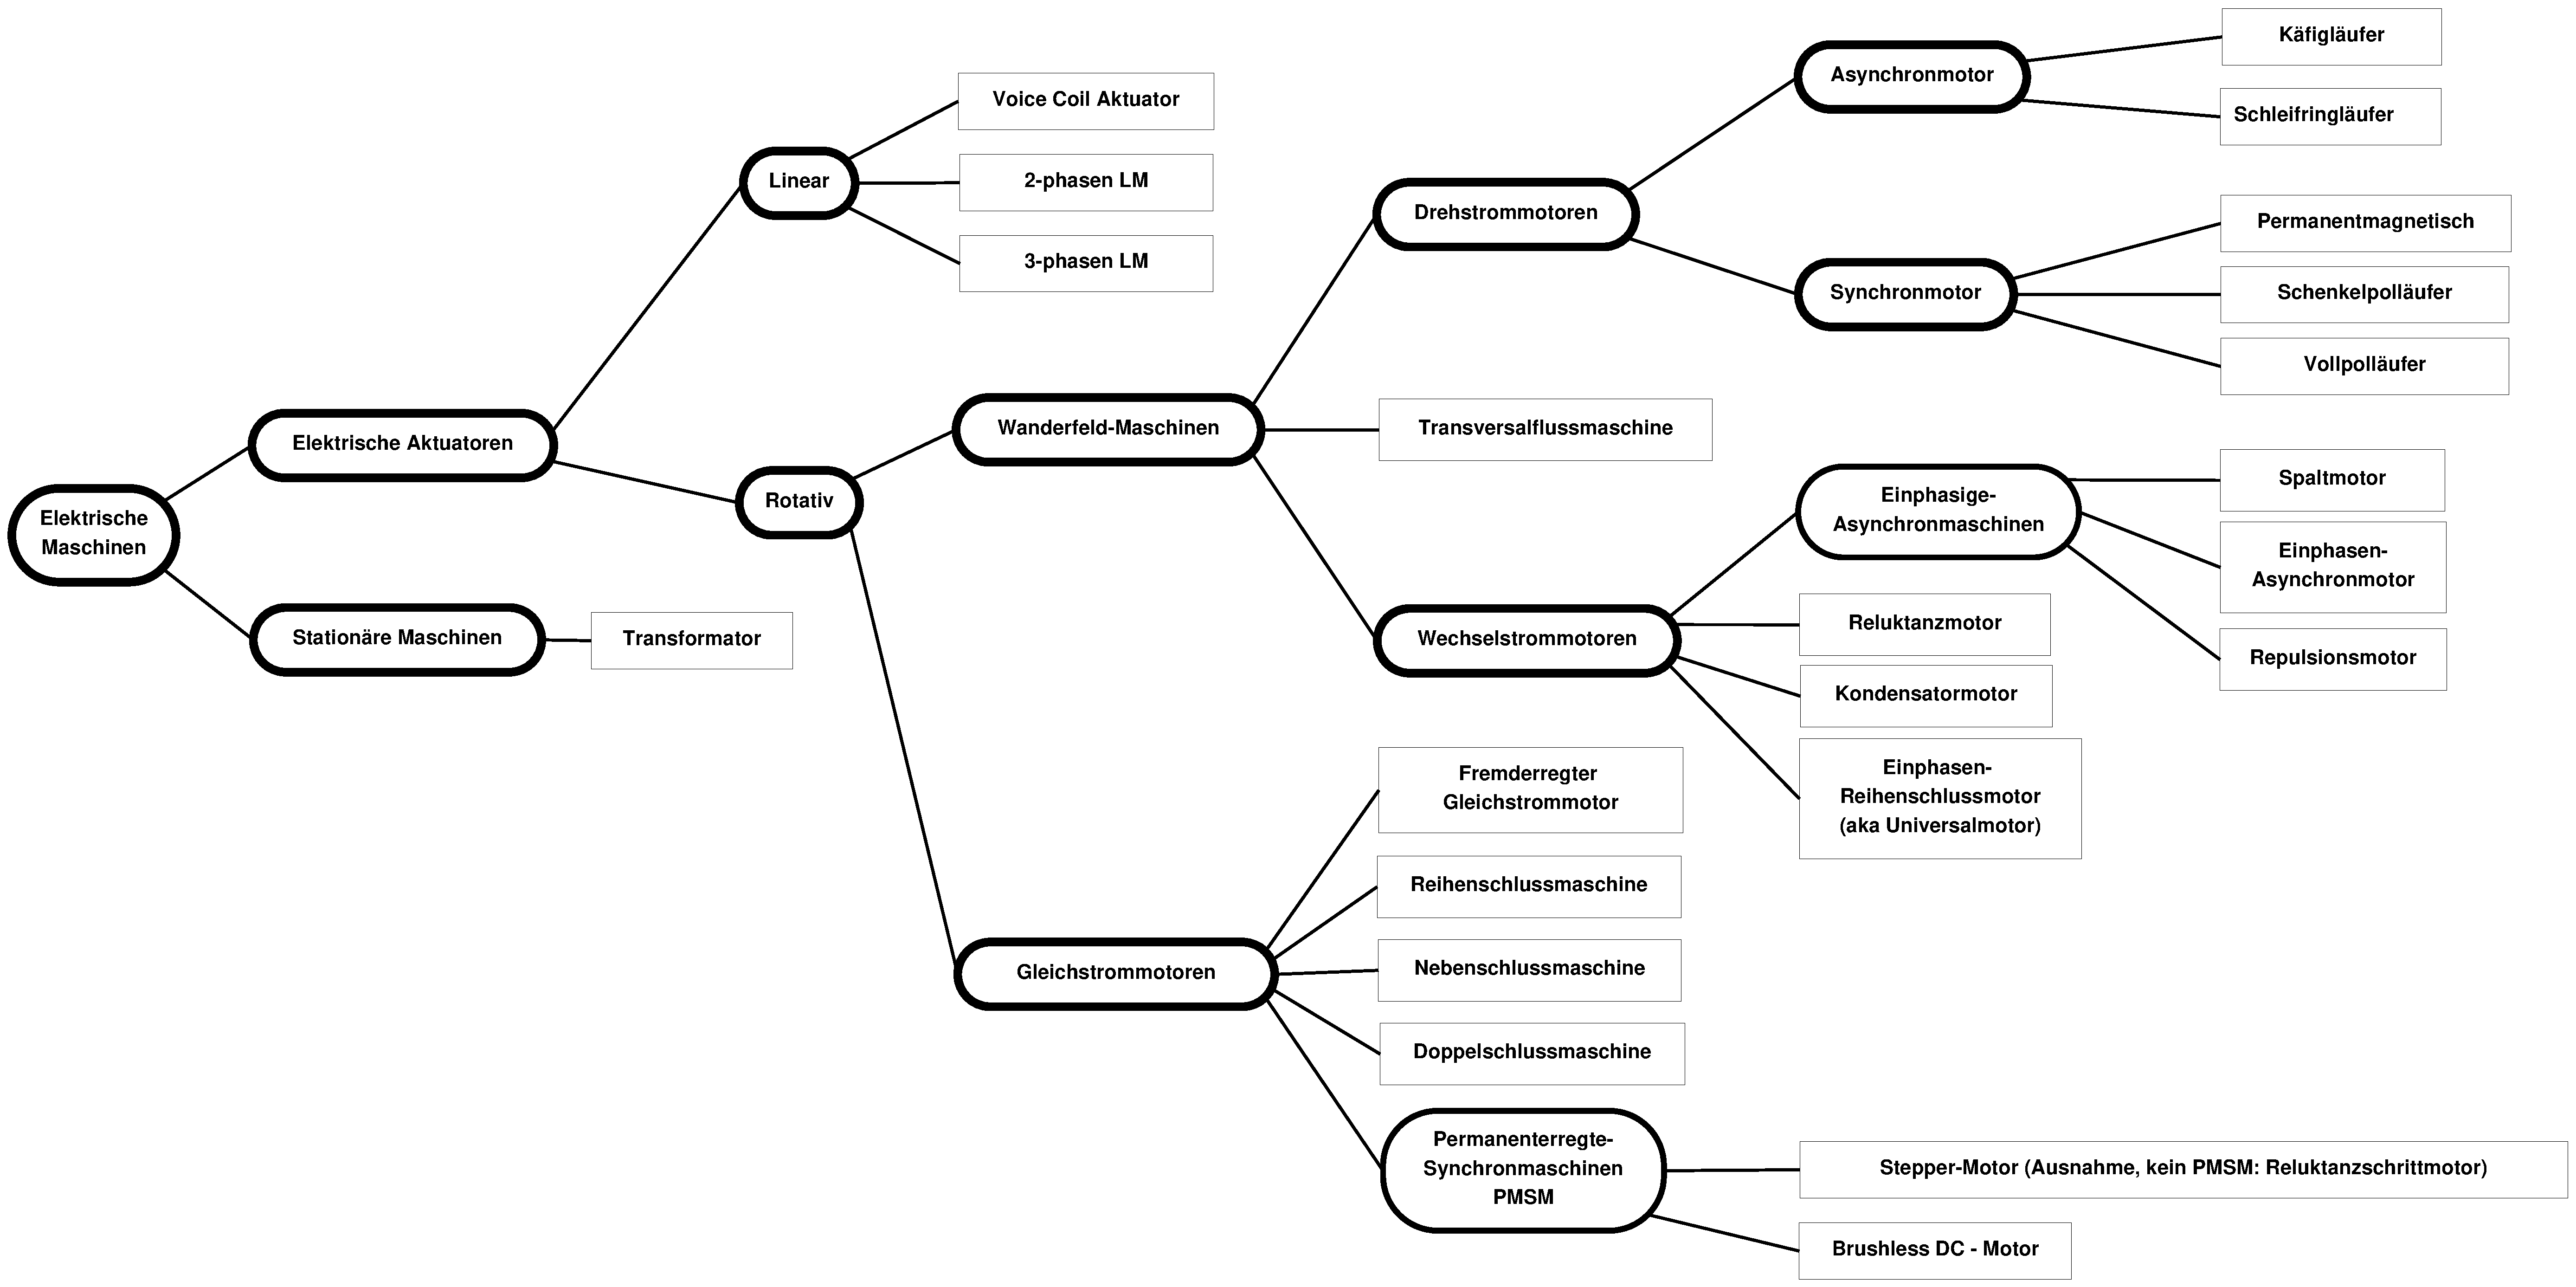
\includegraphics[width=1\linewidth]{./pics/el/elMasch}
		\end{figure}
		\subsection{Stationäre Maschinen}
			\subsubsection{Transformator}
				Ein Transformator besteht meist aus zwei oder mehr Spulen (Wicklungen), die in der Regel aus Kupferdraht gewickelt sind und sich auf einem gemeinsamen Ferrit- bzw. Eisenkern befinden. Ein Transformator wandelt eine Eingangswechselspannung, die an einer der Spulen angelegt ist, in eine Ausgangswechselspannung um, die an der anderen Spule abgegriffen werden kann. Dabei entspricht das Verhältnis von Eingangs- und Ausgangsspannung dem Verhältnis der Windungszahlen der beiden Spulen. So wird zum Beispiel bei einem Windungsverhältnis von 20 zu 1 eine Eingangsspannung von 240 Volt in eine Ausgangsspannung von 12 Volt transformiert. Je nach Auslegung des Transformators kann die Ausgangsspannung somit kleiner, größer oder gleich der Eingangsspannung sein.
				\paragraph*{Wirkprinzip}
					Eine Wechselspannung auf der Primärseite des Transformators bewirkt entsprechend dem Induktionsgesetz einen wechselnden magnetischen Fluss im Kern. Der wechselnde magnetische Fluss wiederum induziert auf der Sekundärseite des Transformators eine Spannung (Spannungstransformation)
					\begin{figure}[h]
					\centering
					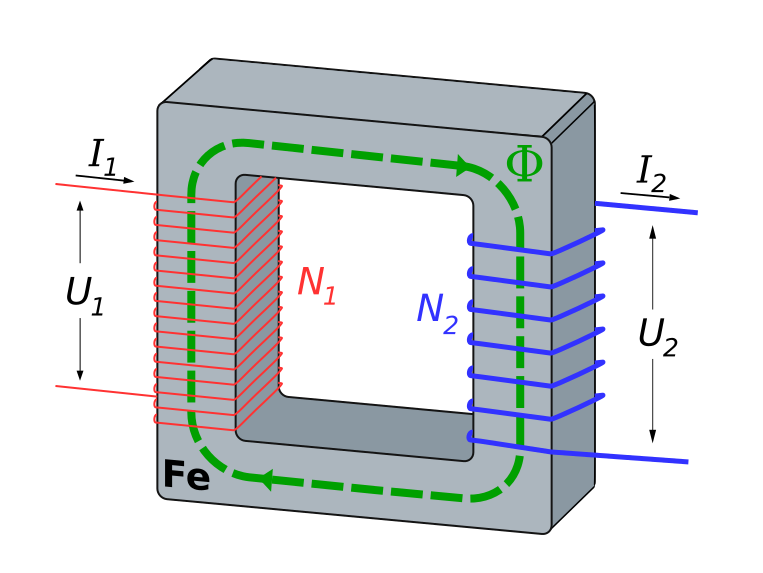
\includegraphics[width=0.4\linewidth]{./pics/el/trafo}
				\end{figure}\\
					Spannungstransformation beim ideal Transformator:\\
					\[\dfrac{U_{2}}{U_{1}}=\dfrac{N_{2}}{N_{1}} \qquad \text{bzw.} \qquad U_{2}=\dfrac{N_{2}}{N_{1}}U_{1}\]
					Wird an die sekundäre Wicklung ein \textbf{Verbraucher angeschlossen}, so entnimmt dieser der Sekundärspule elektrische Energie. Dabei kommt ein Strom auf der Sekundärseite zustande und der Primärstrom vergrößert sich. Im Gegensatz zu den Spannungen an den Wicklungen sind die Ströme in den Wicklungen jedoch entgegengesetzt gerichtet: Wenn der Primärstrom bezogen auf den Kern rechtsherum durch die Spule fließt, fließt der Sekundärstrom linksherum und umgekehrt (Lenzsche Regel).
					\[\dfrac{I_{2}}{I_{1}}=\frac{N_{1}}{N_{2}}\qquad \text{bzw.} \qquad I_{2}=\frac{N_{1}}{N_{2}}I_{1}\]
				\paragraph*{Realer Transformator}
					Ein realer Transformator hat demgegenüber Übertragungsverluste durch den ohmschen Widerstand der Wicklung, durch Wirbelstrombildung im Kern, Ummagnetisierungsverluste und durch andere Effekte. Bei großen Transformatoren muss die Verlustleistung gegebenenfalls durch geeignete Kühlung abgeführt werden. Bei starker Überlastung kann sich ein Transformator überhitzen und "durchbrennen".
					\begin{figure}[h]
						\centering
						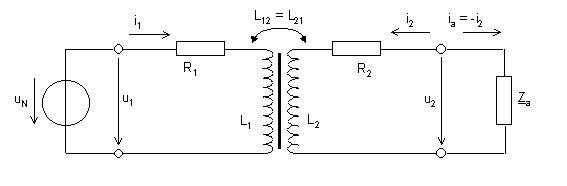
\includegraphics[width=0.7\linewidth]{./pics/el/trafo3}
						\caption{Ersatzschaltbild eines realen Transformators}
					\end{figure}\\
					Die Größen der Sekundärseite können auf die Primärseite mithilfe des Übertragungsfaktors $ \gamma $ umgerechnet werden.
					\[\gamma = \frac{N_{1}}{N_{2}} \quad \rightarrow \quad U'_{2}=U_{2}\gamma, \quad I'_{2}=\dfrac{I_{2}}{\gamma}, \quad L'_{\sigma2}=L_{\sigma2}\gamma^{2}, \quad \underline{Z}'=\underline{Z}\gamma^{2} \]
					Das heißt, ein sekundärseitiger Widerstand $ R $, wirkt primärseitig als $ R\gamma^{2} $.\\\\
					\begin{figure}[h]
						\centering
						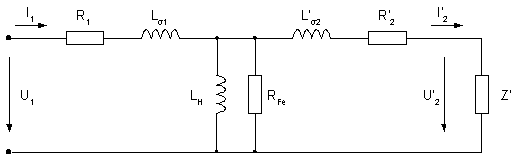
\includegraphics[width=0.7\linewidth]{./pics/el/trafo1.png}
						\caption{Ersatzschaltbild eines realen Transformators mit transformierten sekundärseitigen Größen}
					\end{figure}\\
					\tab[1cm] $R_{1}$\tab...\tab ohmscher Widerstand der Primärwicklung \\
					\tab[1cm] $R_{2}'$\tab...\tab transformierter ohmscher Widerstand der Sekundärwicklung \\
					\tab[1cm] $U_{1}$\tab...\tab primärseitige Spannungsquelle \\
					\tab[1cm] $U_{2}'$\tab...\tab transformierte Ausgangsspannung \\
					\tab[1cm] $Z'$ \tab...\tab transformierte Lastimpedanz \\
					\tab[1cm] $L_{\sigma 1}$\tab...\tab Streuinduktivität der Primärseite \\
					\tab[1cm] $L'_{\sigma 2}$\tab...\tab transformierte Streuinduktivität der Sekundärseite \\
					\tab[1cm] $L_{H}$\tab...\tab Hauptinduktivität, die den Magnetisierungsstrom führt \\
					\tab[1cm] $R_{fe}$\tab...\tab Eisenverluste des Kerns \\
					
				
		\subsection{Elektrische Aktuatoren}
			\leavevmode\\
			\textbf{\large Unterschiede zwischen Eisenlose und eisenbehaftete Motoren\\\\}
			Bei eisenlosen Motoren werden die Wicklungen mit Epoxid vergossen (Luftspaltwicklung). Diese Motoren sind für sehr gleichförmige Bewegungen geeignet. Bei ihnen wird keine magnetische Anziehungskraft erzeugt.
			Bei eisenbehafteten Motoren hingegen werden die Wicklungen in einem Eisenkäfig fixiert. Eisenbehaftete Motoren nutzen das Eisen, um den magnetischen Fluss zu bündeln und können so eine sehr hohe Kraftdichte erzeugen.\\\\			
			\textbf{Vorteile eisenlose Motoren:}
			\begin{itemize}
				\item Keine Eisenverluste (Eisenmagnet muss nicht umgepolt werden, die Hysteresekurve muss nicht durchlaufen werden, was Energie kostet)
				\item Kompakter und leichterer Forcer/Rotor
				\item Kleine Rotor Induktivität (weniger Elektromagnetische Störungen, schnelle Reaktionszeit des Stroms)
				\item Bei Sinuskommutierung erhält man ein gleichförmiges Moment bzw. eine konstant wirkende Kraft
			\end{itemize}
			\leavevmode \\
			\textbf{Vorteile eisenbehaftete Motoren:}
			\begin{itemize}
				\item sehr hohe Drehmomentdichte
				\item Maximierung der magnetischen Kraft
				\item höhere Spitzenkraft als eisenlose Motoren der selben Baugröße ($ \rightarrow $ kompaktere Ausführungen möglich)
			\end{itemize}
			
			\newpage	
			\subsubsection{Linearaktuatoren}				
				\begin{description}[leftmargin=2.5cm]
					\item[Allgemein]					
					Grundsätzlich arbeiten Linearmotoren wie rotatorische Motoren. Man kann sie sich so vorstellen, dass man einen beliebigen Motor aufschneidet und in die Ebene abwickelt.
					\leavevmode \\
					\begin{figure}[h!]
						\centering \rule{1.5cm}{0cm}
						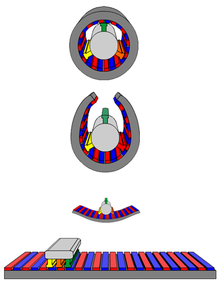
\includegraphics[width=0.2\linewidth]{./pics/el/rot2lin} 
					\end{figure} 
					Wobei die ursprünglich kreisförmig angeordneten elektrischen Erregerwicklungen (Stator) auf einer ebenen Strecke angeordnet sind. Der Läufer, der im Drehstrommotor rotiert, wird beim Linearmotor von dem längs bewegten Magnetfeld über die Fahrstrecke bewegt. Analog dazu funktionieren tubulare Linearmotoren ebenfalls wie ihre rotativen Verwandten, jedoch ist bei Linearmotoren der Untershied einer begrenzten Stator-Streke. Die Idee bei Linearmotoren ist, dass die durch den Motor erzeugte Kraft direkt auf eine zu bewegende Masse wirkt ohne Verluste in Getrieben, Spindeln, Riementrieben, usw. in kauf nehmen zu müssen.
					\begin{figure}[h!]
						\centering 
						
\includegraphics[width=0.05\linewidth]{./pics/el/symbolLinearmotor}
						\caption{Symbol für Linearmotoren}
					\end{figure} \leavevmode \\

					\item[Einteilung]
					\leavevmode \\
					\begin{figure}[h!]
						\centering
						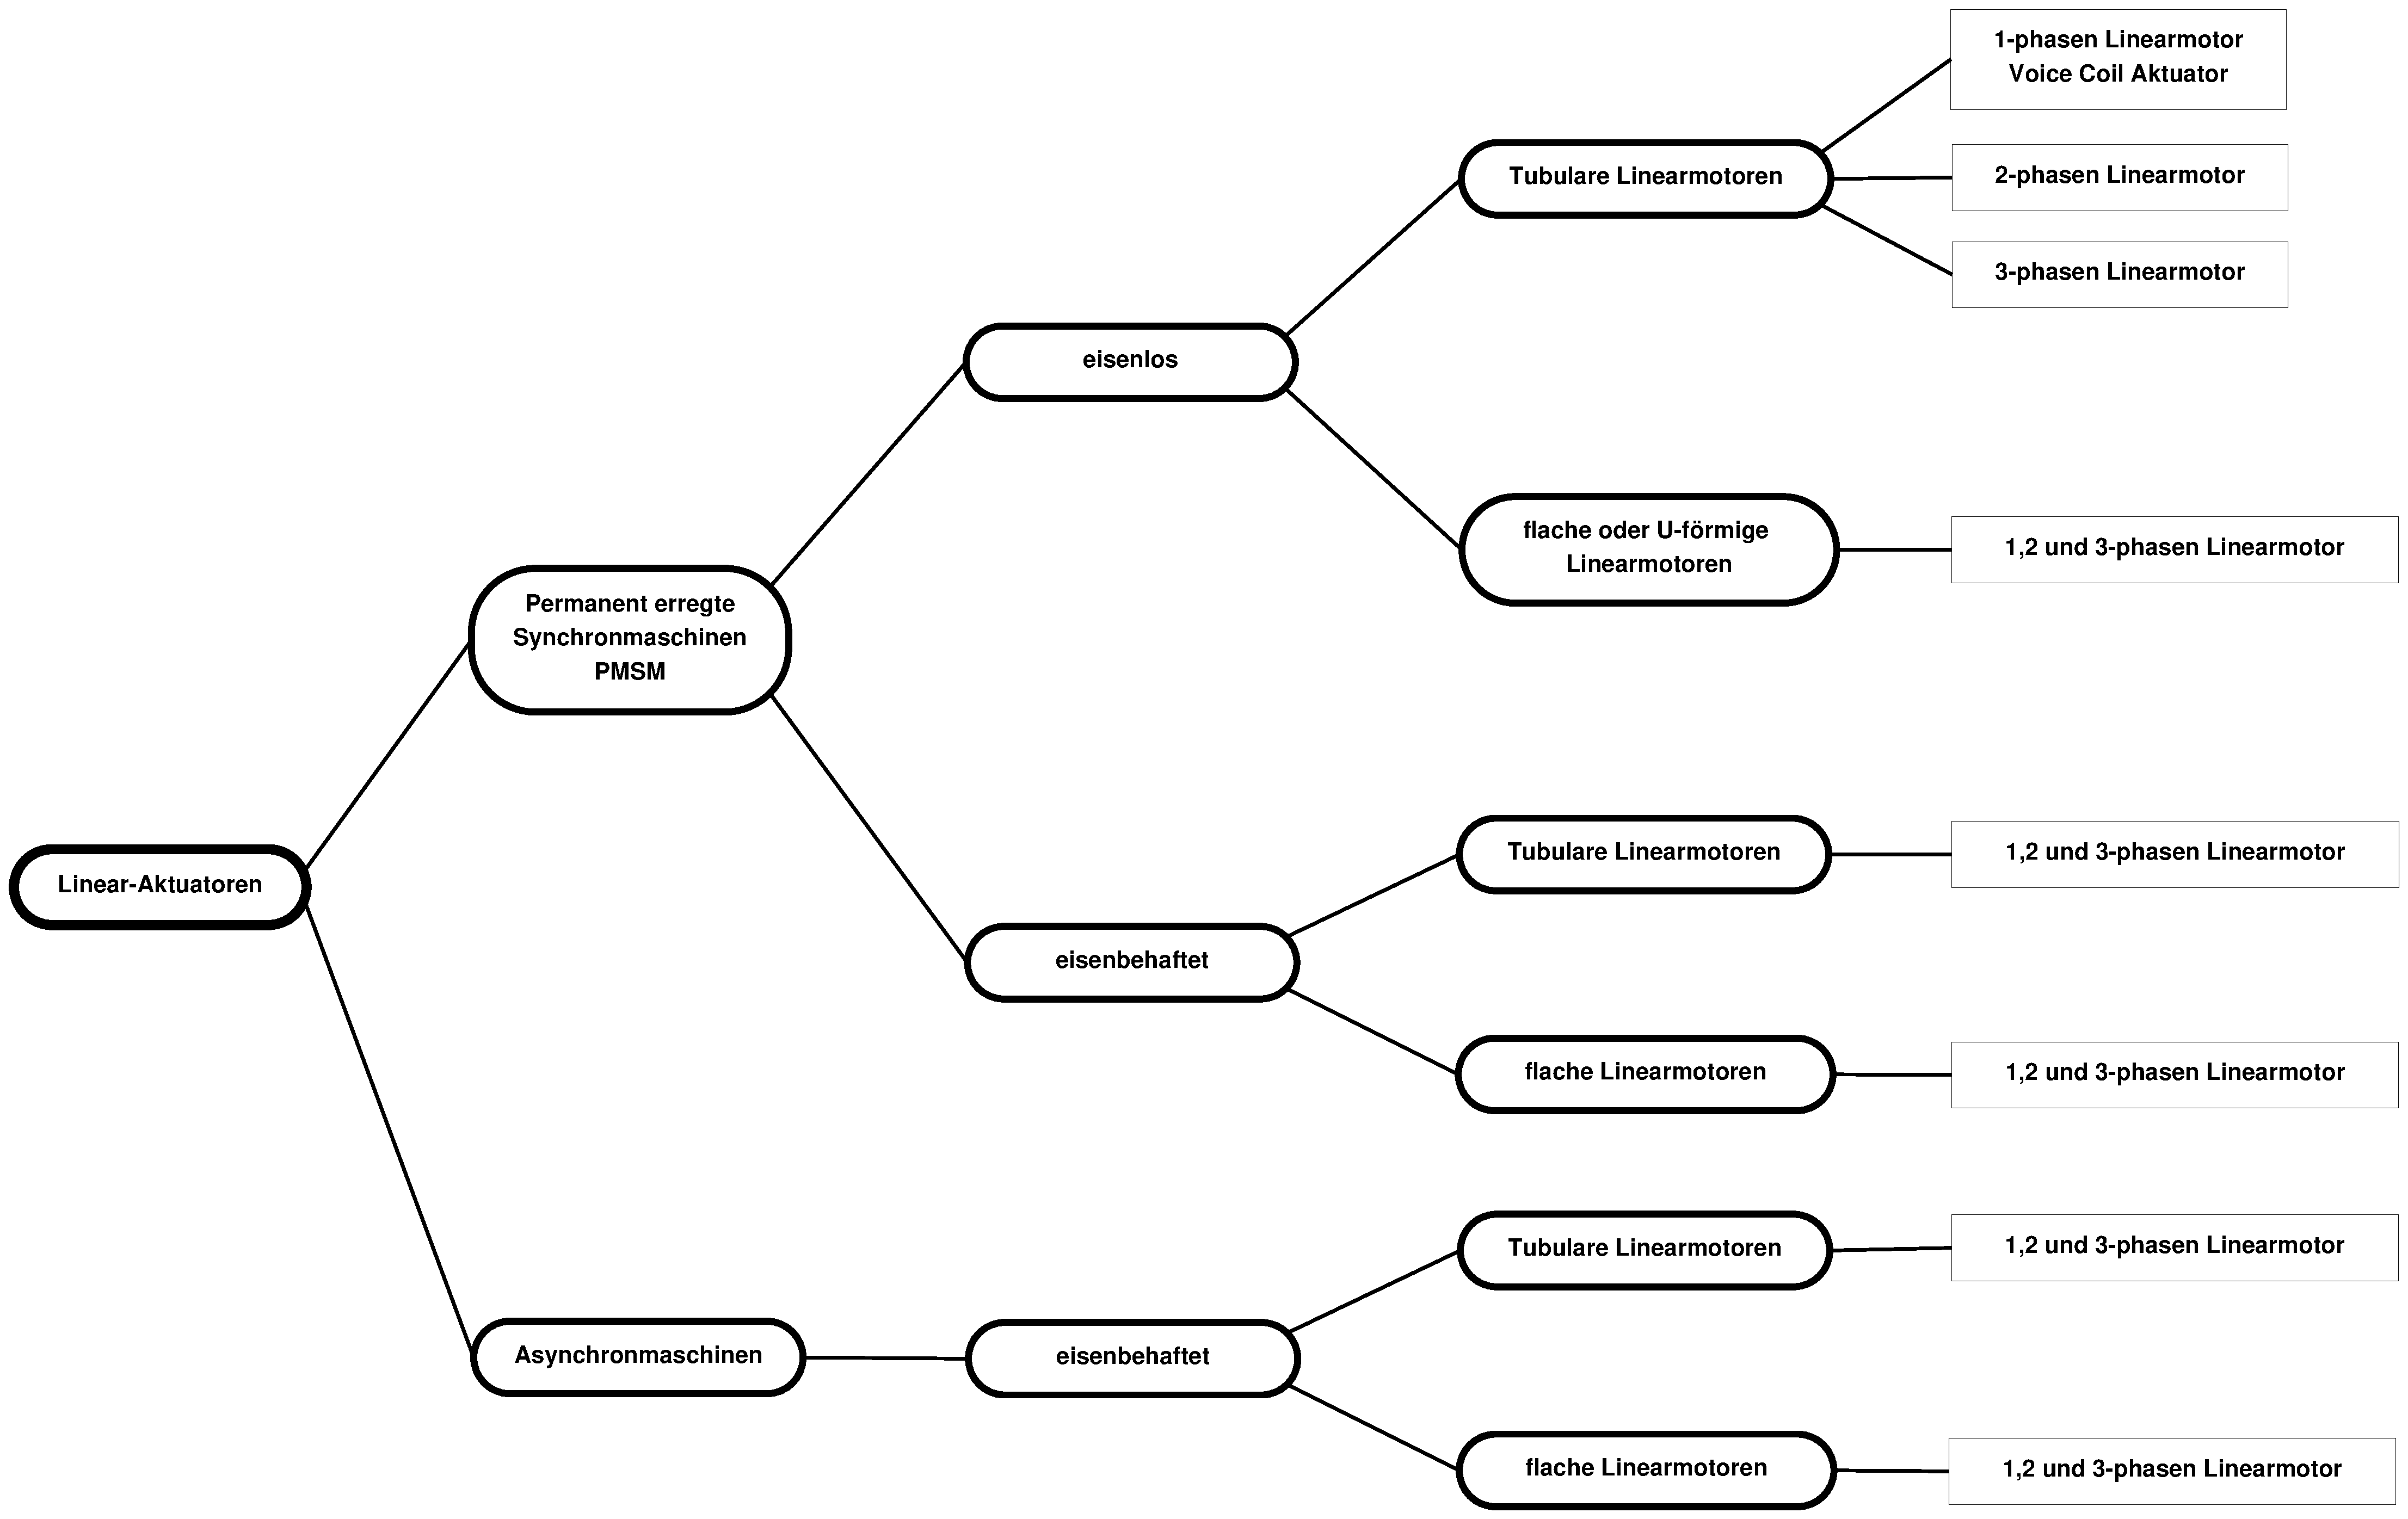
\includegraphics[width=0.9\linewidth]{./pics/el/LinearAktuatoren.eps}
					\end{figure}
				
					\item[Tubulare Linearmotoren] 
					Unter einem tubularen Linearmotor versteht man einen elektrischen Direktantrieb, bei dem die lineare Bewegung direkt aufgrund der elektromagnetischen Kraftwirkung erzeugt wird. Das heißt, die translatorische Bewegung wird nicht durch eine mechanische Umwandlung über eine Spindel, Riemen oder Kurvenscheibe erzeugt, sondern basiert direkt auf den Wechselwirkungen zwischen elektromagnetischen Kräften. Grundsätzlich können derartige Motoren sowohl nach dem Lorenzkraftprinzip wie auch nach dem Maxwellkraftprinzip (siehe Kap. \ref{reluktanzkraft}) aufgebaut werden und gehören zu der Gattung der Linearmotoren. Der Unterschied zu den flachen oder U-förmigen Linearmotoren besteht darin, dass die Erregerwicklung des Stators rohrförmig (tubular) und die Magnete des Läufers stabförmig sind. Konstruktiv gesehen entsteht so ein Antriebselement, das Ähnlichkeiten zu einem pneumatischen oder hydraulischen Zylinder aufweist. Im Bild ist ein permanenterregter Läufer abgebildet. Im asynchronen Fall besteht der Läufer statt aus Permanentmagneten, aus kurzgeschlossenen Kupferwindungen wie beim bekannten rotativen Asynchronmotor.
					\begin{figure}[!h]
						\centering \rule{1.5cm}{0cm}
						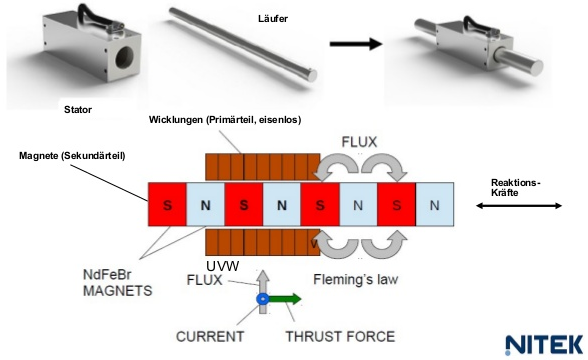
\includegraphics[width=0.55\linewidth]{./pics/el/tubular}
					\end{figure}
					
					\item[Flache, U-förmige Linearmotoren] 
					Bei flachen bzw. U-förmigen Linearmotoren befinden sich bei PMSM die Permanentmagneten am Stator des Motors. Beim asynchronen Linearmotor hält der Stator hingegen die Erregerwicklungen, die um weichmagnetisches Eisen gewickelt sind und somit Magnetfelder erzeugt.	Ein Linearmotor besteht aus nur zwei Komponenten: einem Wicklungspaket (Forcer bzw. Primärteil) und einem Träger (Magnetschiene bzw. Sekundärteil), auf dem die Permanentmagneten fixiert sind. Die Kupferwindungen des Wicklungspaketes sind entweder in Epoxidharz oder Eisen eingebettet. Die Kupferwindungen führen den gesamten Strom eines Linearmotors. 	
					\begin{figure}[h]
						\centering \rule{2.5cm}{0cm}
						\subfigure[U-förmiger Linearmotor]
						 {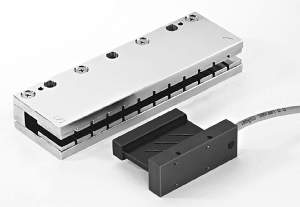
\includegraphics[width=0.4\textwidth]{./pics/el/LM}} \hspace{0.4cm}
						\subfigure[flacher Linearmotor] 
						 {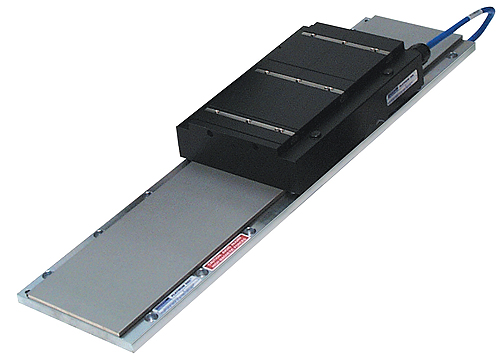
\includegraphics[width=0.4\textwidth]{./pics/el/flatLM}}
					\end{figure}					
					Das Magnetassembly besteht aus Seltenen-Erde-Magneten, die in abwechselnder Polarität auf einem Stahlträger montiert sind. Sie erzeugen ein magnetisches Feld senkrecht zum Träger. Wenn in den Kupferwindungen Strom fließt, ergibt sich nach dem Lorentz´schen Gesetz eine Kraft $ F = I \times B $, die zur Beschleunigung der Masse benutzt wird. Eine Linearmotorachse besteht wiederum aus einem Linearmotor mit Lagerung und einem integrierten Positions-Gebersystem (Encoder). Der Forcer wird üblicherweise an den bewegten Teilen der Maschine befestigt. Das Magnetassembly wird am statischen Teil der Maschine fixiert. 
					\begin{figure}[h]
						\centering \rule{2.5cm}{0cm}
						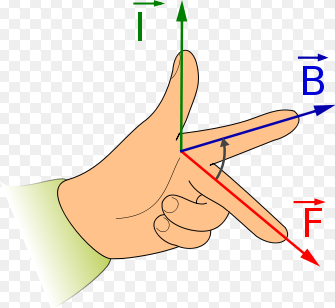
\includegraphics[width=0.2\linewidth]{./pics/el/I.png} \hspace{1cm}
						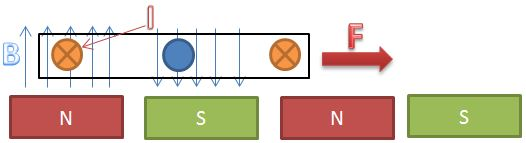
\includegraphics[width=0.5\linewidth]{./pics/el/LM2} 
						\caption{Linke-Hand-Regel für die Wirkrichtung der Lorentzkraft}
						\label{}
					\end{figure}
					
					\item[Asynhroner Linearmotor] 
					Beim linearen Asynchronmotor wird die bewegende Kraft durch ein wanderndes Magnetfeld das mit einem Leiter interagiert, erzeugt. In jedem Leiter, sei es eine Windung, Spule oder einfach nur eine leitende Metallplatte, die im Feld platziert wird, werden Ströme induziert. Durch Wechselwirkung des magnetischen Wanderfeldes und dem induzierten Strom resultiert jene Kraft, die für eine Linearbewegung verantwortlich ist. Asynchrone Linearmotoren werden für Anwendungen die große Kräfte benötigen verwendet. Zum Beispiel elektrisch Schiebetüren oder Magnetschwebebahnen.
					
					\item[PSM als Linearmotor] 
					Die permanenterregte Synchronmaschine (PSM) als Linearmotor benötigt im Forcer einen sinusförmigen Stromverlauf um ohne rucken bewegt werden zu können. Dies kann entweder durch Einspeisung von Wechselstrom erreicht werden oder durch Sinuskommutierung einer Gleichspannung. 
					
					\item[Sinuskommutierung]										
					Ein hoher Gleichlauf kann erreicht werden, indem die Phasenströme graduell angeglichen werden. Der Linearmotor ist geometrisch so aufgebaut, dass sich die Back-EMF in Form einer Sinusspannung ergibt. Daher ist die beste Lösung einen sinusförmigen Stromverlauf vor zu gegeben, der dann zu einer gleichmäßigen Bewegung führt. Das erzeugte Drehmoment/ die erzeugte Kraft ist dann konstant. Einen sinusförmigen Strom nachzubilden verlangt aber eine höhere Positionsauflösung als von den Hallsensoren erhalten werden kann. Der Strom in den 3 Phasen muss viel häufiger angepasst werden. Darum verwendet die Sinuskommutierung meist Encoder zur präzisen Lagebestimmung des Rotors. Sinuskommutierung ermöglicht einen gleichmäßigen Motorbetrieb und ergibt sogar eine bessere Performance.						
				\end{description}
				
				\paragraph{1-phasen Linearmotor/ Linear Voice Coil Motor/ Tauchspulenaktuator}
					Der Voice Coil Aktor ist ein zweipoliger nichtkommutierter Antriebsmechanismus mit limitiertem Weg. Er besteht aus zwei Komponenten: einem Dauermagneten am fixierten Teil und einer Spule, die auf einen im Luftspalt beweglichen nichtmagnetischen Spulenkörper gewickelt ist. Im eingebauten Zustand befindet sich die Spule im Luftspalt des Magnetfeldes. Richtung und Amplitude der Lorentzkraft werden dabei von der Stromstärke und -richtung bestimmt. Sie arbeiten nach dem Lorentz-Kraft-Prinzip und sind dadurch bidirektional aktiv ansteuerbar. Die konstante Kraftverteilung über dem Hub ermöglicht eine hohe Startkraft, die verbunden mit der geringen Masse der bewegten Spule höchste Dynamik erlaubt. Zudem lässt sich eine extrem geringe Hysterese erreichen. Durch diese Eigenschaften empfehlen sich Tauchspulenaktuatoren vor allem für dynamische und präzise Regelungsanwendungen.
					\begin{figure}[h]
						\centering
						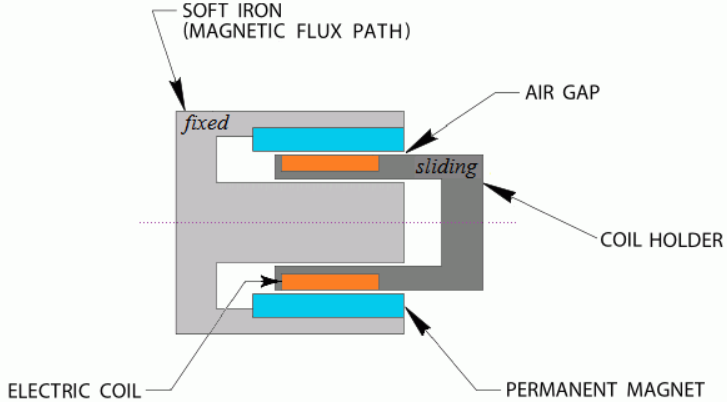
\includegraphics[width=0.6\linewidth]{./pics/el/vcm}
					\end{figure}
					\leavevmode \\
					
				\paragraph{2- und 3-phasen Linearmotor} 
					\begin{description}[leftmargin=2.5cm]
						\item[Bsp. 2-phasen Linearmotor]
						Das Funktionsprinzip ist das selbe wie im Kapitel Linearmotoren erklärt wird. In der Abbildung funktioniert der eisenbehaftete LM nach dem Reluktanzkraft-Prinzip (Kap. \ref{reluktanzkraft}).	\\
						\begin{figure}[h]
							\centering
							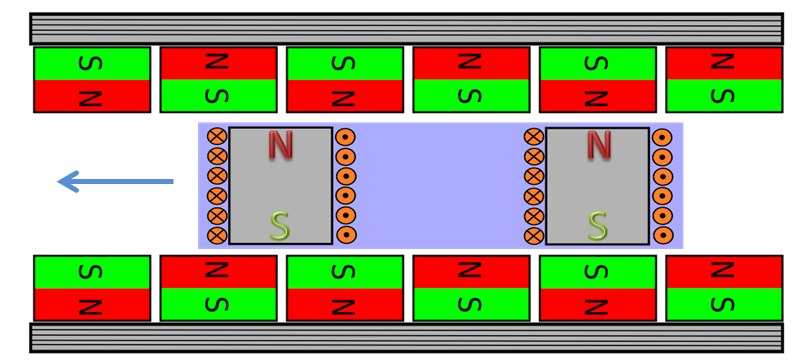
\includegraphics[width=0.6\linewidth]{./pics/el/2phase}
							\caption{2-phasiger, eisenbehafteter, U-förmiger Linearmotor}
						\end{figure} \\
						Die Magnetfelder des Läufers und die des Stators werden immer kombiniert geschaltet (mit Strom versorgt), dass der Läufer vom nächsten Permanentmagnetpol in Bewegungsrichtung ein Wegstück „nach vorne“ gezogen wird (und vom Magnetfeld hinter sich abgestoßen wird). Hat er die Position erreicht, zu der er gezogen wurde, so wird umgepolt, und der Läufer wird von dieser Position nun weggedrückt und zur nächsten Magnetspule/Permanentmagnet hingezogen. Dadurch, dass der Läufer zwei etwas versetzte Magnetfeld-Erzeuger besitzt, befindet sich immer mindestens einer davon gerade „auf halbem Weg“, was eine Festlegung der Laufrichtung (vorwärts oder rückwärts) ermöglicht. Dieser Motor ist die lineare Variante einer permanenterregten Synchronmaschine.
						
						\item[Bsp. 3-phasen Linearmotor]
						Die eisenlosen 3-phasigen elektronisch kommutierten AC synchron
						Linearmotoren sind für die anspruchsvollen Anforderungen
						mit hohen Beschleunigungen sehr gut geeignet. Vorteil der 3-phasigen Linearmotoren ist, dass ein gleichmäßigerer Lauf möglich ist bzw. eine konstante Kraft geliefert werden kann.
						\begin{figure}[h]
							\centering
							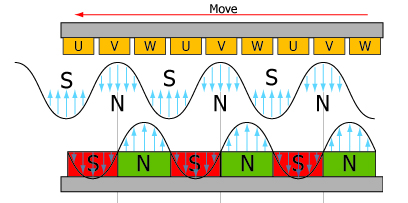
\includegraphics[width=0.7\linewidth]{./pics/el/3phaseLin}
							\caption{eisenloser, permanenterregter, 3-phasen synchron Linearmotor}
						\end{figure}
					\end{description}
					
			\subsubsection{Rotationsaktuatoren}
				\paragraph{Gleichstrommotoren} 
					\subparagraph{Brushless DC-Motor}
						\begin{description}[leftmargin=3cm]
							\item[Aufbau] 
							Der \textit{brushless DC-Motor} basiert entgegen der Namensgebung nicht auf dem Funktionsprinzip der Gleichstrommaschine, sondern ist aufgebaut wie eine Drehstrom-Synchronmaschine mit Erregung durch Permanentmagnete. Die (oft dreisträngige) Drehstromwicklung wird elektronisch kommutiert (z.b. Block- oder Sinuskommutierung). Dadurch entsteht ein sich drehendes magnetisches Feld, welches den permanenterregten Rotor mitzieht.
							\begin{figure}[h]
								\centering \rule{3cm}{0cm}
								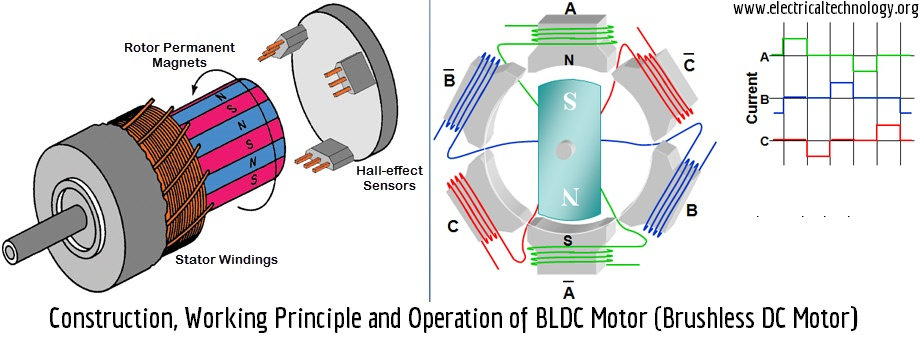
\includegraphics[width=0.82\linewidth]{./pics/el/brushless}
							\end{figure}
							\item[Kommutierungsarten]
							Bei einer Blockkommutierung wird der Strom in den jeweiligen Wicklungen zwischen 3 Zuständen geschaltet. Das sich dabei ergebende Drehmoment weist eine Welligkeit auf. Bei einer Sinuskommutierung ergibt sich hingegen ein konstantes Drehmoment. Die Kommutierung kann entweder mit oder ohne Sensoren erfolgen.
							\begin{figure}[h]
								\centering \rule{1cm}{0cm}
								\includegraphics[width=0.3\linewidth]{./pics/el/blockkomm}
							\end{figure} 
							
							\item[Sensorgesteuerte Kommutierung]
							Bei ersterem werden entweder Hallsensoren oder optische Sensoren verwendet.	Entsprechend dieser Stellungsinformation werden über geeignete Leistungstreiber von der Steuerelektronik die Wicklungen angesteuert, die im Rotor ein Drehmoment erzeugen. Der Vorteil ist, dass die sensorgesteuerte Kommutierung auch bei sehr geringen Drehzahlen bzw. im Stand funktioniert. Gewöhnlich werden bei dieser Kommutierung nicht alle Phasen zugleich bestromt. Bei den Dreiphasenmotoren ist üblicherweise zu jedem Zeitpunkt jeweils eine Phase stromlos.
							
							\item[Sensorlose Kommutierung]
							Bei der sensorlosen Kommutierung erfolgt die Erfassung der Rotorposition über die in den Spulen des Stators induzierte Spannung, welche von der elektronischen Steuerschaltung ausgewertet wird. Allerdings ist zur Auswertung der Induktionsspannung eine gewisse Mindestdrehzahl erforderlich. Sensorlose EC-Motoren müssen daher wie Synchronmotoren bzw. Schrittmotoren bis zum Erreichen der Mindestdrehzahl blind geschaltet werden.
							Mittlerweile gibt es allerdings Verfahren, mit denen ein EC-Motor auch unterhalb dieser Mindestdrehzahl nicht blind gesteuert wird. Dazu werden bei Stillstand kurze Stromimpulse gesendet, die den Motor zwar nicht bewegen, aber durch das magnetische Feld des Rotors beeinflusst werden. Das Magnetfeld mindert oder verstärkt den Stromfluss und verändert so die Zeit, die ein Stromimpuls benötigt, um eine Schwelle zu überschreiten. Diese Zeiten werden gemessen, und man kann damit die Rotorposition schon bei Stillstand bestimmen.
							
							\item[Geeignetste Kommutierung]
							Man erhält für EC-Motoren (electronically commutated) das beste Ergebnis (konst. Kraft), wenn man sie mit ihrer BEMF-Spannung (back electromotive force) ansteuert. Diese Spannung kann an bzw. zwischen den Phasen gemessen werden, wenn man den Motor "von Hand" bewegt.
							
							\item[Unterschied zur PMSM]
							Die BEMF ergibt bei PMSM einen sinusoidalen Spannungsverlauf. Bei BLDC hingegen einen trapezförmigen Spannungsverlauf der Gegeginduktionsspannung. Die Verläufe folgern aus den unterschiedlichen Statorwicklungen. Bei BLDC sind die Wicklungen konzentriert und bei PMSM hingegen viel gleichmäßiger auf den Umfang verteilt, was zu einer sinusoidalen Spannung führt. Dadurch Unterscheidt sich auch die Ansteuerung der beiden Motoren, da man die höchste Performance erreicht indem man den Motor mit der selbigen Spannung als seine BEMF ansteuert.
							\begin{figure}[h]
								\centering 
								\includegraphics[width=0.27\linewidth]{./pics/el/bldcpmsm}
								\includegraphics[width=0.45\linewidth]{./pics/el/sinus}
								\caption{PMSM- sinusoidale BEMF}
							\end{figure}
						\end{description}
	
					\subparagraph{Steppermotor}
						\begin{description}[leftmargin=3cm]
							\item[Allgemein]
							Ein Schrittmotor ist ein Synchronmotor, bei dem der Rotor  durch ein gesteuertes, schrittweise rotierendes, elektromagnetisches Feld der Statorspulen um einen minimalen Winkel (Schritt) oder sein Vielfaches gedreht werden kann. Schrittmotoren existieren auch in Form von Linearmotoren. Schrittmotoren folgen im Prinzip exakt dem außen angelegten Feld und können ohne Sensoren zur Positionsrückmeldung (Encoder, Drehgeber oder ähnliches) genau betrieben werden. Sie sind haben ein ähnliches Verhalten wie Synchronmotoren, weisen aber in der Regel eine deutlich höhere Polpaarzahl auf. Daher können sie einfacher betrieben werden als beispielsweise Servomotoren, da diese auf die gewünschte Position eingeregelt werden müssen. Für einen besonders homogenen Verlauf werden Schrittmotoren mit einem gleichförmigen Drehfeld angesteuert.
							\begin{figure}[h]
								\centering \rule{2.5cm}{0cm}
								\subfigure[Schema mit 4 Schritten pro Umdrehung und unipolarer Beschaltung]
								{\includegraphics[width=0.45\textwidth]{./pics/el/stepper}} \hspace{0.4cm}
								\subfigure[Reluktanzschrittmotor] 
								{\includegraphics[width=0.35\textwidth]{./pics/el/StepperMotor.png}}
							\end{figure}	
							
							\item[Schrittverlust] 
							Wird ein Schrittmotor durch ein externes Lastmoment oder durch die anzutreibende Masse beim starken Beschleunigen beziehungsweise Verzögern überlastet (d. h. Lastmoment > Motormoment), kann der Rotor dem Drehfeld nicht mehr folgen. Es werden Schritte übersprungen, und die Information über die aktuelle Position des Rotors geht verloren. Bei diesem sogenannten Schrittverlust springt der Motor in die vorherige oder nächste Position gleicher Phase zurück. Durch die mechanische Bewegungsenergie (Trägheit) kommt es bei rasch bewegten Magnetfeldern meist zu einer Serie von verlorenen Schritten. Auftretende Schrittverluste summieren sich und führen dann zu einer ungenauen Positionierung.
							
							\item[Bauarten]
							\begin{itemize}
								\item Reluktanzschrittmotor
								\item Permanentmagnetschrittmotor
								\item Hybridschrittmotor (Reluktanz- und Permantmagnetschrittmotor)
								\item Lavet-Schrittmotor
							\end{itemize}
						
							\item[Reluktanzschrittmotor]
							Beim Reluktanzschrittmotor besteht der Rotor aus einem gezahnten Weicheisenkern. Bei diesem Material verschwindet nach dem Ausschalten des Statorstromes das Magnetfeld. Bei eingeschaltetem Strom fließt der magnetische Fluss durch den Weicheisenkern des Rotors. Die Drehbewegung des Rotors kommt zustande, weil vom gezahnten Stator der nächstliegende Zahn des Rotors angezogen wird, da sich so der magnetische Widerstand verringert. Da der Reluktanzschrittmotor keine Permanentmagnete enthält, hat er daher im Gegensatz zum Permanentmagnetschrittmotor bei ausgeschaltetem Strom auch kein Rastmoment.
							
							\item[Permanentmagnetschrittmotor]
							Beim Permanentmagnetschrittmotor besteht der Stator aus Weicheisen und der Rotor aus Dauermagneten, die abwechselnd einen Nord- und einen Südpol aufweisen. Mit dem Stator-Magnetfeld richtet man den dauermagnetischen Rotor so aus, dass eine Drehbewegung entsteht. Beim Permanentmagnetschrittmotor ist die Anzahl der Pole (und damit die Auflösung) begrenzt.
							
							\item[Hybridschrittmotor]
							Der Hybridschrittmotor vereint die positiven Eigenschaften beider Bauformen durch feine Schrittteilung und gutes Drehmoment. Sein Rotor besteht aus einem axialen Permanentmagneten, an dessen Enden (Polen) gezahnte Weicheisenkränze befestigt sind. Beide sind um eine halbe Zahnbreite gegeneinander versetzt, so das sich Nord- und Südpole abwechseln. Vorteil ist das erheblich kleinere äußere Magnetfeld. Nahezu alle heute erhältlichen Schrittmotoren sind Hybridmotoren, da er hohe mechanische Leistungen bei kleinen Schrittwinkeln und kleiner Bauform vereint. Die gebräuchlichsten Schrittauflösungen liegen zwischen 50 und 2000 Schritte pro Motorumdrehung ohne elektronische Zusatzmaßnahmen. Bezüglich der Phasenzahl sind 2-Phasenmotore am gängigsten.
							\begin{figure}[h]
								\centering \rule{1.5cm}{0cm}
								\includegraphics[width=0.4\linewidth]{./pics/el/hybrid}
							\end{figure}
						
							\item[Ansteuerung \& Anschluss]
							Weiterhin kann man zwei Gruppen von Motoren bzw. Ansteuertechniken unterscheiden: Unipolare und bipolare Motoren. Unipolare Motoren verfügen über zwei Spulen mit Mittelabgriff. Sie haben fünf oder sechs Anschlüsse. Mit einem Multimeter läßt sich schnell feststellen, welche Anschlüsse die Mittelabgriffe und welche die Spulenenden sind. Die Ansteuerung erfolgt durch wechselweises Einschalten von jeweils einem Spulenende, so daß immer nur die halbe Spule bestromt ist.
							Ein 2-phasiger, bipolarer Motor hat zwei Spulen, manchmal auch zwei Spulenpaare, die durch Umpolen angesteuert werden. Sind zwei Spulenpaare vorhanden (also acht Anschlüsse am Motor), können die Spulenpaare wahlweise parallel oder in Reihe geschaltet werden, woraus sich unterschiedliche (dynamische) Eigenschaften ergeben. Eine Parallelschaltung führt im allgemeinen zu mehr Drehmoment im oberen Drehzahlbereich, stellt aber auch höhere Anforderungen an den Stromregler. Bipolare Motoren mit 8 Anschlüssen können prinzipiell auch unipolar angesteuert werden, wobei man allerdings einen Teil der Motorperformance verschenkt.
							\begin{figure}[h]
								\centering \rule{1.5cm}{0cm}
								\includegraphics[width=0.7\linewidth]{./pics/el/unibipolar}
								\caption{Anschlussvarianten eines 2-phasigen Steppermotors}
							\end{figure} 
							Bei der Beschaltung der Spulen ergeben sich drei weitere Betriebsarten: Vollschritt- Wavedrive- und Halbschrittbetrieb.
							\begin{enumerate}
								\item Normal-Betrieb: Es werden immer beide Spulen gleichzeitig bestromt. Es ergeben sich vier unterschiedliche Schrittpositionen (siehe Schaubild) pro Umlauf.
								\item Wavedrive-Betrieb: Hier wird immer nur eine Spule bestromt. Die Leistungsaufnahme und damit auch das Drehmoment sind im Vergleich zu 1) geringer. Die resultierenden vier Schrittpositionen liegen zwischen denen aus 1).
								\item Halbschritt-Betrieb: Kombination aus 1) und 2). Es wird wechselweise eine, bzw. zwei Spulen bestromt. Es ergeben sich 8 Schrittpositionen. Daher kommt die Bezeichnung Halbschritt, da der physikalische Schrittwinkel des Motors halbiert wird.
							\end{enumerate}		
							\begin{figure}[h]
								\hspace{3.2cm}
								\begin{minipage}{0.75\textwidth}		
								\centering 
								\includegraphics[width=1\linewidth]{./pics/el/vollschritt}
								\caption{Oberen vier Zustände: Wavedrive-Betrieb, unteren vier Zustände: Vollschrittbetrieb,		Halbschrittbetrieb: alle 8 Zustände}
								\end{minipage}
							\end{figure} 							
						
							\item[Vor- \& Nachteile gegenüber BLDC]
							\hspace{0.5cm}
							\begin{minipage}[t]{0.38\textwidth}
								\textbf{Steppermotor}
								\begin{itemize}
									\item[+] Günstiger als BLDC (Preis-Leistung)
									\item[+] Einfache Winkel-(Weg-)messung durch Schrittzählung ohne Encoder möglich
									\item[-] Moment nimmt ab einer bestimmten Drehzahl ab	
									\item[-] nur niedrige Drehzahlen möglich
																	
								\end{itemize}
							\end{minipage}
							\hspace{0.5cm}
							\begin{minipage}[t]{0.35\textwidth}
								\textbf{Brushless DC-Motor}
								\begin{itemize}
									\item[+] Hohe Drehzahlen
									\item[+] Sehr gute Laufruhe
									\item[+] günstiger Momentenverlauf über den gesamten zulässigen Drehzahlbereich
									\item[-] Kostet mehr als Stepper
									\item[-] Encoder nötig für Weg-, Drehzahlmessung
								\end{itemize}
							\end{minipage}	
						
							\item[Anwendungszwecke]
							Typische Anwendungsgebiete sind Drucker, vor allem Matrixdrucker, oder der Antrieb des Schreib-/Lesekopfes in einem Diskettenlaufwerk. Aufgrund ihrer hohen Genauigkeit werden sie auch in computergesteuerten Werkzeugmaschinen zur Positionierung der Werkzeuge verwendet. Durch die ständig sinkenden Kosten für die Ansteuerelektronik werden sie auch zunehmend im Konsumgüterbereich verwendet. So sind in Kraftfahrzeugen der mittleren und gehobenen Kategorie heute bis über 50 Schrittmotoren im Einsatz, die Betätigung der vielen Klappen einer automatischen Heizungs- und Klimaanlage ist dafür ein Beispiel. Schrittmotoren können bis ungefähr 1 kW wirtschaftlich eingesetzt werden.
																		
						\end{description}
						
					\subparagraph{Servomotor}
						Als Servomotor werden Elektromotoren beliebiger Bauart (AC, DC) bezeichnet, die die Kontrolle der Winkelposition, Drehzahl und Winkelbeschleunigung ihrer Motorwelle erlauben. Bürstenlose Servomotoren sind entweder Brushless DC-Motoren, Drehstrom-Asynchronmotoren oder Drehstrom-Synchronmotoren. Sie bestehen aus einem Elektromotor, der zusätzlich mit einem Sensor (Encoder) zur Positionsbestimmung ausgestattet ist. Die vom Sensor ermittelte Winkelposition/ -geschwindigkeit der Motorwelle wird kontinuierlich an eine meist außerhalb des eigentlichen Motors angebrachte Regelelektronik übermittelt, den so genannten Servoregler, der die Bewegung des Motors entsprechend einem oder mehreren einstellbaren Sollwerten, wie etwa Soll-Winkelposition oder Solldrehzahl, regelt.
						\begin{figure}[h]
							\centering
							\includegraphics[width=0.5\linewidth]{./pics/el/servo}
							\caption{Die Kombination Servomotor und Servoregler wird als Servoantrieb bezeichnet}
	
						\end{figure}
						
					\subparagraph{Torque-Motor} 
						Torque-Motoren können als Außenläufer (Stator innen, Rotor außen) oder normale Innenläufer ausgeführt sein. Durch den verhältnismäßig großen Durchmesser, die hochpoligen Wicklungen können diese Motoren große Drehmomente bei geringen Drehzahlen erzeugen. Meist werden BLDC-Motoren als Torquemotoren gebaut, teilweise aber auch Reluktanzmotoren.
						\begin{itemize}
							\item[+] Große Beschleunigungen möglich $ \rightarrow $ hohe Dynamik des Systems
							\item[+] Antriebssteif $ \rightarrow $ kein Verdrehspiel $ \rightarrow $ geringere Störgrößen $ \rightarrow $ gute Regeleigenschaften
							\item[+] Kaum Verschleiß
							\item[-] Starke Wärmeentwicklung (muss oft Wassergekühlt werden)
							\item[-] Teuer
						\end{itemize}
						\begin{figure}[h]
							\centering
							\includegraphics[width=0.5\linewidth]{./pics/el/TM}
						\end{figure}
						
				\paragraph{Drehstrommotoren} 
					\subparagraph{\textcolor{red}{Synchronmotor}}						
						Mn und Pn Kurven, vergleich mit asynchron!!!
					\subparagraph{\textcolor{red}{Asynchronmotor}}
				\paragraph{\textcolor{red}{Wechselstrommotoren}} 
					\subparagraph{\textcolor{red}{Reluktanzmotor}}
					\subparagraph{...}
\part{\textcolor{red}{Regelungstechnik}}
\section{Begrifflichkeiten}
	\begin{center}
		\begin{tabular}{l|p{12cm}}
			\textbf{Begriff} & \textbf{Beschreibung} 
			\\\hline & \\
			eingangsaffine Systeme & sind Systeme die in \textit{u} linear sind. Man sagt auch 		eingangslineare Systeme. \\& Genauer bedeutet es, dass sich die wirkende Stellgröße \textit{u} nur linear über die Zeit ändert.
			\\ & \\ \hline & \\
			relativer Grad $ \delta $ eines Systems & bei SISO-Sytemen gibt der relative Grad gleich dem Grad der Ableitungen der Ausgangsgröße $ y $ an, bei dem die $ \delta-$mal abgeleitete Ausgangsgröße erstmals direkt von der Stellgröße $ u $ abhängt: $ y^{(\delta)}_{i}=fcn(u) $. Ist der rel. Grad eines Systems \textit{wohldefiniert}, dann ist es Eingangs-/Ausgangs-linearisierbar. Für lineare Systeme entspricht der relative Grad dem Differenzgrad des Zähler- und Nennerpolynoms.  Der
			relative Grad r auch als die Anzahl der Integratoren gedeutet werden, die der Eingang u
			durchlaufen muss, bevor er den Ausgang y beeinflusst. In anderen Worten wird der Ausgang $ y^{(\delta)} $ direkt vom Eingang $ u $ beeinflusst und der Ausgang $ y $ erst über $ \delta $ Integratoren. Der relative Grad r ist somit ein Maß
			für die Mindestverzögerung im E/A-Verhalten.\\& [\textsc{Nichtlineare Systeme und Regelungen, Jürgen Adamy S290}]
			\\ & \\ \hline & \\
			Transitionsmatrix $ \bm{\Phi}(t) \label{transitionsmatrix} $& Die Transitionsmatrix  $ \bm{\Phi}(t) $ beschreibt den Übergang des Zustandsvektors $ \bm{x}(t) $	von seinem Anfangswert $ \bm{x}_{0} $ zu seinem Wert zum Zeitpunkt t.\\ & $\bm{x}(t) = \bm{\Phi}(t)\bm{x}_{0} +\int_{0}^{t}\bm{\Phi}(\tau -t)\bm{Bu}(\tau)d\tau $
			\\ & \\ \hline & \\
			Diffeomorphismus \label{diffeomorphismus} & Ist eine nichtlineare Zustandstransformation $ \bm{z} = \bm{q}(\bm{x}), \quad \bm{x} = \bm{q}^{-1}(\bm{z}) $ die stetig differenzierbar und eindeutig ist. Letzteres bedeutet, dass jedem $ \bm{x} $ kann genau ein $ \bm{z} $ zugeordnet werden und umgekehrt.
			\\ & \\ \hline & \\
			
			
			
		\end{tabular}
	\end{center}
\section{Eigenschaften von Systemen}
	\subsection{Flachheit}
		Ist ein System \textit{flach}, so können die dynamischen Gleichungen des Systems so umgeformt werden, dass sich Eingangs- und Zustandsgrößen anhand von Funktionen darstellen die nur von den Ausgangsgrößen und deren Ableitungen abhängig sind. Dadurch ist es möglich für einen gewünschten Ausgangsgrößenverlaufs die nötigen Eingangs- und Zustandsgrößenverläufe direkt anzugeben. \\\\
		\textit{Beispiel}:
		\begin{eqnarray} 
			\dot{x}_{1}&=& x_{2}\nonumber\\
			\dot{x}_{2}&=& -x_{1}-x_{2}+u\nonumber\\
			y&=&x_{1}\nonumber
		\end{eqnarray}
		Die Zustandsgrößen des Systems können als Funktionen der der Ausgangsgrößen dargestellt werden.
		\[\bm{x}=\begin{bmatrix}x_{1}\\x_{2}\end{bmatrix} = \begin{bmatrix}y\\\dot{y}\end{bmatrix} \]
		Ebenso der Eingangsvektor aus der mittleren Gleichung.
		\[u=\ddot{y}+\dot{y}+y\]
		Bei einem solchen System wird \textit{y} als \textbf{flacher Ausgang} bezeichnet. Dabei ist es nicht relevant ob dieser Ausgang tatsächlich existiert oder nur ausgedacht - \textit{fiktiv} ist. Existieren nur \textit{fiktive} flache Ausgänge müssen diese für den Entwurf einer Steuerung in den realen Ausgang umgerechnet werden.\\
		\begin{tcolorbox}[title=Definition: Flachheit]
			Für Systeme
			\[\bm{\dot{x}}=\bm{f(x,u)}, \quad \bm{x}\in \mathbb{R}^{n}, \bm{u}\in \mathbb{R}^{m}  \]
			mit $ m\leq n $ (weniger Eingangs- als Zustandsgrößen) für die sich keine Stellgröße $ u_{i} $ als Funktion anderer Stellgrößen $ u_{j\neq i} $ darstellen lässt
			\[rang\bigg(\dfrac{\partial\bm{f(x,u)}}{\partial\bm{u}}\bigg)=m, \]
			ist die \textit{Flachheit} folgendermaßen definiert:
			\tcblower
			Es heißt flach wenn ein realer oder fiktiver Ausgangsvektor	
			\[\bm{y} = \bm{h}(\bm{x,u,\dot{u},...,u}^{\alpha})\]
			existiert, so dass\\\\	
			\textit{(1) der Zustandsvektor $ \bm{x} $ als Funktion von $ \bm{y} $ und einer endlichen Anzahl $ \beta $ von Ableitungen von $ \bm{y} $}
			\[\bm{x} =\bm{\varPsi}_{1}(\bm{y,\dot{y},...,y}^{(\beta)}) \]
			\textit{dargestellt werden kann,}\\\\
			\textit{(2) der Eingangsvektor $ \bm{u} $ als Funktion}
			\[\bm{u} =\bm{\varPsi}_{2}(\bm{y,\dot{y},...,y}^{(\beta+1)}) \]
			\textit{darstellbar ist,}\\\\
			\textit{(3) für Ein- und Ausgangsvektor}
			\[dim(\bm{y}) = dim(\bm{u})\]
			gilt.
		\end{tcolorbox}	
	
	
\section{Systemtransformationen}
	\subsection{Zustandstransformation}
		Die Wahl der Zustandsgrößen eines Systems sind keinesfalls eindeutig. Mit Hilfe einer \textit{Zustandstransformation} kann ein System in eine neue Systemdarstellung mit neuen Zustandsgrößen transformiert werden.
		\subsubsection{Lineare Zustandstransformation}
			Durch eine \textit{reguläre Zustandstransformation} der Form
			\[\bm{x}(t) = \bm{Vz}(t)  \]
			mit der regulären Matrix $ \bm{V} $ (reguläre Matrix: invertierbare, quadratische Matrix) lässt sich ein \textit{Axbu-Modell} mit dem Zustand $ \bm{x}(t) $ in die Form
			\[\bm{\dot{z}} = \bm{V}^{-1}\bm{AVz} + \bm{V}^{-1}\bm{Bu} \]
			\[\bm{y} = \bm{CVz} + \bm{Du} \]
			mit dem neuen Zustand $ \bm{z} $ überführen. Eine solche Transformation kann beispielsweise verwendet werden um die Dynamikmatrix $ \bm{A} $ in eine Diagonalmatrix umzuwandeln. Damit kann auf einfache Weise die \hyperref[transitionsmatrix]{Transitionsmatrix} $ \bm{\Phi}(t) $ berechnet und mit $ \bm{V} $ wieder in die ursprüngliche Zustandsdarstellung überführt werden.
			\[ \bm{\Phi}(t) = \bm{V}^{-1}\tilde{\bm{\Phi}}(t)\bm{V} \] 
			\begin{figure}[h]
				\centering
				\includegraphics[width=0.4\linewidth]{./pics/re/zsttrans}
				\caption{Reguläre Zustandstransformation}
			\end{figure}
			\leavevmode \\
			Auch wird die Matrix $ \tilde{\bm{A}}= \bm{V}^{-1}\bm{AV}$ gerne in eine Begleitmatrix der Form
			\[ \tilde{\bm{A}} = \begin{bmatrix}0 & 1 & 0 & \dotsm & 0 \\
			0 & 0 & 1 & \dotsm & 0 \\
			\vdots & \vdots & \vdots & \ddots & \vdots\\
			0 & 0 & 0 & \dotsm & 1 \\
			-a_{0} & -a_{1} & -a_{2} & \dotsm & -a_{n-1} \\\end{bmatrix}\]
			umgewandelt, da diese Darstellungen nützlich für den Reglerentwurf sind (als Beispiel sei die Polvorgabe gegeben) oder Systemeigenschaften direkt abgelesen werden können.
			
		\subsubsection{Nichtlineare Zustandstransformation}
			Auch bei nichtlinearen Systemen
			\[\bm{\dot{x}} = \bm{f}(\bm{x,u}) \]
			können Transformationen
			\[\bm{z} = \bm{q}(\bm{x}), \qquad \bm{x} = \bm{q}^{-1}(\bm{z}) \]
			sinnvoll sein, wenn es gelingt, das System in eine für den Reglerentwurf geeignete Form zu bringen. Für die Transformation wird gefordert, dass sie stetig differenzierbar und eindeutig ist. Eindeutig bedeutet, dass jedem $ \bm{x} $ genau ein $ \bm{z} $ zugeordnet ist und umgekehrt. Dadurch ist auch gefordert, dass die Anzahl der Zustände durch eine nichtlineare Zustandstransformation gleich bleibt. Eine solche Transformation nennt man \hyperref[diffeomorphismus]{Diffeomorphismus}. Das transformierte System ergibt sich durch Substitution zu
			\[\dfrac{\partial \bm{q}^{-1}(\bm{z})}{\partial \bm{t}}  = \bm{f}(\bm{q}^{-1}(\bm{z}),\bm{u}) 
			\qquad \Rightarrow \qquad
			\dfrac{\partial \bm{q}^{-1}(\bm{z})}{\partial \bm{z}} \dot{\bm{z}} = \bm{f}(\bm{q}^{-1}(\bm{z}),\bm{u}),  \] 
			woraus sich die transformierte Systemdarstellung 
			\[\Rightarrow \qquad 
			 \dot{\bm{z}} = \bigg(\dfrac{\partial \bm{q}^{-1}(\bm{z})}{\partial \bm{z}}\bigg)^{-1}\cdot \bm{f}(\bm{q}^{-1}(\bm{z}),\bm{u}) = \tilde{\bm{f}}(\bm{z,u}) \]
			 ergibt. Da die Transformation eindeutig ist, gibt es auch eine Rücktransformation
			 \[ \dot{\bm{x}} = \bigg(\dfrac{\partial \bm{q}(\bm{x})}{\partial \bm{x}}\bigg)^{-1}\cdot \bm{\tilde{f}}(\bm{q}(\bm{x}),\bm{u}) = \bm{f}(\bm{x,u}). \]
			 Im allgemeinen kann es sein, dass die Transformationsgleichung auch eine Abhängigkeit vom Eingangsvektor $ \bm{u} $ und eventuell seinen zeitlichen Ableitungen aufweist. D.h. die Form
			 \[\bm{z} = \bm{q}(\bm{x,u,\dot{u}, ...,u}^{(i)}) \]
			 \[\bm{x} = \bm{q}^{-1}(\bm{z,u,\dot{u}, ...,u}^{(i)}) \]
			 hat. Transformiert man nun das System $ \bm{\dot{x}} = \bm{f}(\bm{x,u}) $ in z-Koordinaten, erhält man
			 \[\dot{x} = \dfrac{\partial \bm{q}^{-1}(\bm{z,u,\dot{u}, ...,u}^{(i)})}{\partial t}= 
			 \dfrac{\partial \bm{q}^{-1}(\bm{z,u,\dot{u}, ...,u}^{(i)})}{\partial z}\dot{z} +\sum_{j=0}^{i}\dfrac{\partial \bm{q}^{-1}(\bm{z,u,\dot{u}, ...,u}^{(i)})}{\partial \bm{u}^{(j)}}\bm{u}^{(j+1)}=
			 \bm{f}(\bm{q}^{-1}(\bm{z,u,\dot{u}, ...,u}^{(i)}),\bm{u}) \]
			 und schließlich die transformierte Systembeschreibung
			 \[\Rightarrow \bm{\dot{z}} = 
			 \bigg(\dfrac{\partial \bm{q}^{-1}(\bm{z,u,\dot{u}, ...,u}^{(i)})}{\partial z}\bigg)^{-1}\cdot \bigg(\bm{f}(\bm{q}^{-1}(\bm{z,u,\dot{u}, ...,u}^{(i)}),\bm{u}) -  \sum_{j=0}^{i}\dfrac{\partial \bm{q}^{-1}(\bm{z,u,\dot{u}, ...,u}^{(i)})}{\partial \bm{u}^{(j)}}\bm{u}^{(j+1)}\bigg). \]
			 Mit dem Hintergedanken dass die Zustände $ \bm{x} $ bzw. $ \bm{z} $ auch vom Eingang und seinen Ableitungen abhängt, kann die transformierte folgendermaßen dargestellt werden.
			 \[\Rightarrow \bm{\dot{z}} = 
			 \bigg(\dfrac{\partial \bm{q}^{-1}}{\partial z}\bigg)^{-1}\cdot \bigg(\bm{f}(\bm{q}^{-1},\bm{u}) -  \sum_{j=0}^{i}\dfrac{\partial \bm{q}^{-1}}{\partial \bm{u}^{(j)}}\bm{u}^{(j+1)}\bigg) = \tilde{\bm{f}}(\bm{z,u})\]
			 
			 \textsc{Nichtlineare Systeme und Regelungen, Jürgen Adamy S207}
			 \paragraph{Herleitung des Diffeomorphismus (Transformationsvorschrift \textit{ q})}
			 TODO				
			
	\subsection{Eingangstransformation}
		
\section{Stabilität}
	\subsection{Stabilitätsanalyse des charakteristischen Polynoms}	
		Bei linearen Systemen ist das Nennerpolynom der Übertragungsfunktion das charakteristische Polynom, wobei dessen Koeffizienten die Nullstellen des Polynoms und somit die Pole des Systems darstellen. Gegeben sei die Differentialgleichung
		\[\dot{y}(t) + a_{0}y(t) = 0. \]
		Mit dem eulerschen Ansatz $ y=e^{\lambda t} $ ergibt sich
		\[e^{\lambda t}(\lambda + a_{0}) = 0\]
		mit dem charakteristischen Polynom $ \lambda + a_{0} = 0 $. Dieses Polynom hat die Nullstelle 
		\[\lambda=-a_{0}.\]
		In den Ansatz eingesetzt ergibt sich
		\[ y(t)=e^{-a_{0} t}. \]
		Dadurch ergibt sich für unendliche Zeit und einem negativen Realteil von $ a_{0} $
		\[\lim\limits_{t\mapsto \infty}(e^{-a_{0} t}) = 0.\]
		Die Differentialgleichung heißt dann asymptotisch stabil. Für Differentialgleichungen höherer Ordnungen werden etwa das \textit{Hurwitz}- oder \textit{Routh}-Kriterium verwendet um die stabilität von DGL's zu prüfen.
	
\section{Eigenschaften eines Regelkreises}
	\subsection{Bandbreite}
		Die Bandbreite eines Regelkreises ist jene Frequenz, bei der der Amplitudenverlauf des Bode Diagramms, die -3dB Grenze unterschreitet. Höhere Bandbreite bedeutet, dass der Regelkreis (das geregelte System) seinem Sollwert bis zu höheren Frequenzen folgen kann.
		\begin{figure}[h]
			\centering
			\includegraphics[width=0.7\linewidth]{./pics/re/band}
			\caption{Amplitudenverlauf: $ \omega_{B} $ - Bandbreite des Systems, $ \omega_{K} $ - Knickfrequenz}
			\label{}
		\end{figure}
		\leavevmode \\
	
	\subsection{\textcolor{red}{Nyquist-Diagramm}}
	\subsection{\textcolor{red}{Wurzelortskurve}}
	\subsection{\textcolor{red}{Empirische Grundformeln}}
	\subsection{Führungs- und Störungsverhalten eines Regelkreises}


\section{Identifikation von Systemen}

\section{Systemdarstellung: Normal- und Regelungsformen}
	\subsection{Normalformen}
	\subsubsection{Regelungsnormalform \textit{(auch Steuerungsnormalform)}}
	\subsubsection{Beobachtungsnormalform}
	\subsubsection{Kanonische Normalform}
	\subsubsection{Brunovsky–Normalform}
	\subsubsection{Jordansche-Normalform}
	\subsubsection{Nichtlineare Regelungsnormalform} \label{chapNL}
		Nichtlineare eingangsaffine Systeme der Form
		\begin{equation}
			\dot{\bm{x}}=\bm{a(x) + B(x)}\cdot u =\bm{a(x)}+\sum_{i=1}^{m}\bm{b}_{i}(u)\cdot u_{i}
			\label{nlrnf}
		\end{equation}

		können in der nichtlinearen Regelungsnormalform
		\[\begin{bmatrix}\dot{x}_{1}\\\vdots\\ \dot{x}_{n-1}\\\dot{x}_{n}\end{bmatrix} =
		\begin{bmatrix}x_{2}\\\vdots\\ x_{n}\\\alpha(\bm{x})\end{bmatrix} + 
		\begin{bmatrix}0\\\vdots\\ 0\\\beta(\bm{x})\end{bmatrix}u\]
		\[y = x_{1}\]	
		dargestellt werden.
		\begin{figure}[h]
			\centering
			\includegraphics[width=0.6\linewidth]{./pics/re/nlrnf}
			\caption{System in nichtlinearer Regelungsnormalform}
			\label{}
		\end{figure}
		\paragraph{Zustandskoordinatentransformation mittels Lie-Ableitungen}
			Im folgenden wird beschrieben, wie Systeme der Form (\ref{nlrnf}) in die nichtlineare Regelungsnormalform transformiert werden können.\\
			\begin{tcolorbox}[title=Definition: \textit{Lie-Derivierte/Lie-Ableitung}]
				Sie sind als Gradient einer skalaren Funktion $ h(\bm{x}) $ multipliziert mit einem Vektorfeld $ \bm{f(x)} $ definiert
				\[\bm{L_{f}}h(\bm{x}) = \dfrac{\partial h(\bm{x})}{\partial\bm{x}}\bm{f(x)}=grad^{T}h(\bm{x})\cdot \bm{f(x)} \]	
				Die skalare Funktion kann beispielsweise die Ausgangsfunktion $ c(\bm{x}) $ sein und das Vektorfeld z.b. der Dynamikvektor $ \bm{a}(\bm{x}) $.
			\end{tcolorbox}
			Man bildet nun die zeitliche Ableitung der Ausgangsgröße $ y $ und erhält
			\[\dot{y}=\dfrac{dc(\bm{x(t)})}{dt} = \dfrac{\partial c(\bm{x})}{\partial x_{1}}\underbrace{\dfrac{\partial x_{1}(t)}{\partial t}}_{\dot{x}_{1}} + ... + \dfrac{\partial c(\bm{x})}{\partial x_{n}}\dot{x}_{n} = \dfrac{\partial c(\bm{x})}{\partial \bm{x}}\dot{\bm{x}}.\]
			Durch einsetzen von $ \dot{\bm{x}}=\bm{a(x) + b(x)}\cdot u $ in obige Gleichung, ergibt sich  
			\[\dot{y}=\dfrac{\partial c(\bm{x})}{\partial \bm{x}}\bm{a(x)} + \dfrac{\partial c(\bm{x})}{\partial \bm{x}}\bm{b(x)}\cdot u. \]
			Geschrieben mit den Lie-Derivierten:
			\[\dot{y}=L_{\bm{a}}c(\bm{x})+ L_{\bm{b}}c(\bm{x})\cdot u \]
			Für die meisten technischen Systeme ist der zweite Term gleich Null, woraus 
			\[\dot{y}=L_{\bm{a}}c(\bm{x})\]
			folgt.
			Die zweite Ableitung ergibt sich dann zu
			\[\ddot{y}= \dfrac{dL_{\bm{a}}c(\bm{x})}{dt}= \dfrac{\partial L_{\bm{a}}c(\bm{x})}{\partial \bm{x}}\dot{\bm{x}} = \underbrace{\dfrac{\partial L_{\bm{a}}c(\bm{x})}{\partial \bm{x}}\bm{a(x)}}_{L_{\bm{a}}L_{\bm{a}}c(\bm{x})}+\underbrace{\dfrac{\partial L_{\bm{a}}c(\bm{x})}{\partial \bm{x}}\bm{b(x)}}_{L_{\bm{b}}L_{\bm{a}}c(\bm{x})}\cdot u = L_{\bm{a}}L_{\bm{a}}c(\bm{x}) + L_{\bm{b}}L_{\bm{a}}c(\bm{x})\cdot u.\]
			Mit dem zweiten Term wieder zu Null folgt
			\[\ddot{y}=L_{\bm{a}}L_{\bm{a}}c(\bm{x}) = L_{\bm{a}}^{2}c(\bm{x})\]
			Bildet man auch die höheren Ableitungen, so ergibt sich schließlich folgendes Ergebnis:
			\begin{eqnarray} 
				y &=& c(\bm{x})\nonumber\\
				\dot{y}&=&L_{\bm{a}}c(\bm{x})\nonumber\\
				\ddot{y}&=&L_{\bm{a}}^{2}c(\bm{x})\nonumber\\
				\vdots \nonumber\\
				y^{(\delta-1)} &=&L_{\bm{a}}^{(\delta-1)}c(\bm{x})   \nonumber\\
				y^{(\delta)} &=&L_{\bm{a}}^{(\delta)}c(\bm{x}) + L_{\bm{b}}L_{\bm{a}}^{(\delta-1)}c(\bm{x})\cdot u   \nonumber\\
			\end{eqnarray}
			Leitet man die Ausgangsfunktion $ \delta- $mal, so dass die Stellgröße $ u $ darin auftaucht, nennt man $ \delta $ den relativen Grad des Systems. Es wird nun lediglich der Fall
			\[\delta = n\]
			betrachtet, also der Fall bei dem der relative Grad gleich der Systemordnung entspricht.
			Weiter führen wir die neuen Zustandskoordinaten $ \bm{z} $ ein.
			\[\bm{z}=\begin{bmatrix}z_{1}\\z_{2}\\z_{3}\\\vdots\\ z_{n}\end{bmatrix} = 
			\begin{bmatrix}y\\\dot{y}\\\ddot{y}\\\vdots\\ y^{(n-1)}\end{bmatrix} =
			\begin{bmatrix}c(\bm{x})\\L_{\bm{a}}c(\bm{x})\\L_{\bm{a}}^{2}c(\bm{x})\\\vdots\\ L_{\bm{a}}^{(n-1)}c(\bm{x})\end{bmatrix} = \bm{t}(\bm{x})\]
			Ist $ \bm{t}(\bm{x}) $ stetig differenzierbar und es existiert die Umkehrfunktion 
			\[\bm{t}^{-1}(\bm{t}(\bm{x}))=\bm{x},\]
			dann nennt man $ \bm{t} $ einen \textit{Diffeomorphismus}. Durch Differenziation der Transformationsgleichung $ bm{t}(\bm{x}) $ erhalten wir die nichtlineare Regelungsnormalform.
			\[\bm{\dot{z}}=\begin{bmatrix}\dot{z}_{1}\\\dot{z}_{2}\\\dot{z}_{3}\\\vdots\\ \dot{z}_{n}\end{bmatrix} = \begin{bmatrix}\dot{y}\\\ddot{y}\\\dddot{y}\\\vdots\\ y^{(n)}\end{bmatrix} = \begin{bmatrix}z_{2}\\z_{3}\\z_{4}\\\vdots\\ z_{n+1}\end{bmatrix} =\bm{\dot{t}}(\bm{x}) = \begin{bmatrix}L_{\bm{a}}c(\bm{x})\\L_{\bm{a}}^{2}c(\bm{x})\\\vdots\\ L_{\bm{a}}^{(n-1)}c(\bm{x})\\ L_{\bm{a}}^{(n)}c(\bm{x}) + L_{\bm{b}}L_{\bm{a}}^{(n-1)}c(\bm{x})\cdot u\end{bmatrix}\]
			\[\Rightarrow\begin{bmatrix}\dot{z}_{1}\\\vdots\\\dot{z}_{n-1}\\ \dot{z}_{n}\end{bmatrix} = \begin{bmatrix}z_{2}\\\vdots\\ z_{n}\\\alpha(\bm{x})\end{bmatrix}+\begin{bmatrix}0\\\vdots\\ 0\\\beta(\bm{x})\end{bmatrix}u,\]
			mit
			\begin{eqnarray} 
			\alpha(\bm{x}) &=& L_{\bm{a}}^{(n)}c(\bm{x}) \nonumber\\
			\beta(\bm{x}) &=& L_{\bm{b}}L_{\bm{a}}^{(n-1)}c(\bm{x}) \nonumber
			\end{eqnarray}
			
	\subsubsection{Byrnes-Isidori-Normalform}
	
	
\section{Arten von Regelstrecken}
	\begin{itemize}
		\item  linear, nichtlinear
		\item statisch, dynamische
		\item zeitvariant, zeitinvariant
		\item SISO, MIMO
	\end{itemize}

\section{Arten von Reglern}
	\begin{itemize}
		\item Realisierung als Analoger- und digitaler Regler
		\item Stetige lineare Regler
		\begin{itemize}
			\item PID-Regler
			\item Zustandsregler
		\end{itemize}
		\item Unstetige Regler
		\begin{itemize}
			\item Zweipunktregler
			\item Dreipunktregler
			\item Mehrpunktregler
		\end{itemize}
		\item Nichtlineare Regler
		\begin{itemize}
			\item Adaptiver Regler
			\item Fuzzy-Regler
		\end{itemize}
	\end{itemize}
	\subsection{Standardregelkreis}
		Der Standardregelkreis ist ein Regelkreis mit Ausgangsrückführung. Dabei wird lediglich das Eingangs-/Ausgangsverhalten des Systems betrachtet. Die Regelstrecke kann auch als Zustandsraummodell mit Zustandsvariablen beschreiben werden, jedoch wird
		\begin{figure}[h]
			\centering
			\includegraphics[width=0.7\linewidth]{./pics/re/std}
			\caption{Standardregelkreis mit Ausgangsrückführung}
		\end{figure}
		Regler können anhand von Frequenzlinienverfahren oder durch vorgeben der Zähler- und Nennerpolynome der Übertragungsfunktion (Polvorgabe) entworfen werden. Bei vorhandener Übertragungsfunktion kann mittels inverser Laplace-Transformation der zeitliche Verlauf der Ausgangsgröße errechnet und durch die Parameterwahl vorgegeben werden. 
	\subsection{Zustandsregler}
		Der \textit{Standardregelkreis} und dazugehörige Frequenzkennlinienverfahren beruhen auf einer Regelkreisstruktur, bei der eine Größe, die so genannte Ausgangsgröße, gemessen wird, und auf deren Kenntnis gemeinsam mit der vorgegebenen Führungsgröße der Regler als dynamisches System die Stellgröße errechnet. Daher werden Regelkreise dieser Art auch als Ausgangsregelungen bezeichnet. Setzt man nun voraus, dass der gesamte Zustand eines Systems messtechnisch erfassbar ist, dann ist es möglich, einen so genannten \textit{Zustandsregler} zu entwerfen. Die Zustandsvariablen eines Systems sind frühzeitiger als der Ausgang vorhanden, was zu einer schnellen Regelung führt.
		\begin{figure}[h]
			\centering
			\includegraphics[width=0.7\linewidth]{./pics/re/zust}
			\caption{Zustandsregler mit $ h^{T} $ zur Vorgabe der Systemdynamik und $ V $ zur Elimination des statischen Fehlers}
		\end{figure}
		\leavevmode\\
		Durch die Hintereinanderschaltung der Integratoren ist nur die Zustandsvariable x1(t) = y(t) eine stationäre Größe, wenn die Eingangsgröße 	$ 	u ( t )$ konstant ist. Alle anderen Zustandsvariablen – eine stabile Regelstrecke vorausgesetzt – streben gegen den Wert null. Nach Einstellung und Optimierung des Faktors k1 ergibt sich ein stabiler Regelkreis bestimmter Dämpfung mit einem Proportionalfehler der Regelgröße	$ y ( t ) $	gegenüber 
		$ 	w ( t ) $. Die anderen Faktoren der Zustandsvariablen werden hintereinander beispielsweise zur Optimierung des Übergangsverhaltens eingestellt.
		Ein Vorfilter vor dem Soll-Ist-Vergleich korrigiert den statischen Fehler zwischen $ 	w ( t ) $ und 	$ 	y ( t ) $. Durch Einfügen eines überlagerten PI-Reglers verschwinden die Nachteile des einfachen Zustandsreglers. Das Vorfilter wird dann nicht mehr benötigt.\\\\
		Durch die Zustandsrückführung kann keine stationäre Genauigkeit der Regelgröße zum Sollwert erreicht werden. Selbst bei einer Regelstrecke ohne Nullstellen, also ohne differenzielle Anteile, ist die Zustandsvariable $ x_{1} $ nach der Regelungsnormalform nicht identisch mit der Ausgangsgröße $ y(t) $. Deshalb wird die Zustandsrückführung häufig mit einem Vorfilter $ V $ erweitert. Die Führungsgröße $ w ( t ) $ wirkt direkt auf das Vorfilter. Für einfache Anforderungen kann mittels eines Faktors in dem Vorfilter eine Korrektur durchgeführt werden, damit im stationären Zustand $ 	w ( t ) = y ( t ) $ erreicht wird.

\section{Auslegung von Reglern}
	\subsection{Reglerauslegung durch Polvorgabe}
	\subsection{Frequenzkennlinienverfahren}

\section{Arten von Rückführungen}
	\subsection{Ausgangsrückführung}
		Die klassische Ausgangsrückführung $ \bm{u}=\bm{K(w-y)} $ stand am Anfang der Entwicklung der Regelungstechnik. Diese Art der Rückführung wird meist im \textsc{laplace}-Bildbereich untersucht und es spielt dabei nur das Eingangs-/Ausgangsverhalten eine Rolle.
	\subsection{Zustandsrückführung}
		Für komplexere Regelungsaufgaben kommen Zustandsrückführungen zum Einsatz.
		\[\bm{u}=\bm{R_{u1}x}+\bm{R_{u2}v}\]
		Sie ist die allgemeinere Rückführungsart der Beiden und umfasst somit auch die Ausgangsrückführung. Betrachtungen von Zustandsmodellen finden meist im Zeitbereich statt. Hauptanwendungen sind \textit{exakte Linearisierungen} oder \textit{Entkoppelungen} die das System in mehrere Teilsysteme aufteilt, die dann unabhängig voneinander gesteuert oder geregelt werden können.
		\subsubsection{Statische Zustandsrückführung}
			Bei der statischen Zustandsrückführung ist charakteristisch, dass die Eingangsgröße $ \bm{u} $ von den Zustandsgrößen und der neuen Eingangsgröße $ \bm{v} $ abhängig ist.
			\[\bm{u}=\bm{r(x)}+\bm{R(x)v}\]
			\begin{figure}[h]
				\centering
				\includegraphics[width=0.6\linewidth]{./pics/re/stat}
				\caption{Statische Zustandsrückführung; $ \Sigma_{ALS} $ bedeutet \textit{analytisches Modell mit linear eingehender Steuerung}}
			\end{figure}
		\subsubsection{Quasi-statische Zustandsrückführung}
			Bei der quasi-statischen Rückführung ist $ \bm{u} $ zusätzlich von den Ableitungen des neuen Eingangs $ \bm{v} $ abhängig. Jedoch wird der Zustandsvektor nicht wie bei der dynamischen Rückführung erweitert, sondern behält seine Dimension.
		\subsubsection{Dynamische Zustandsrückführung}
			Bei der dynamischen Rückführung treten zusätzliche Differentialgleichungen in einer neuen internen Variable $ z $ auf. Ist die neue Eingangsgröße $ \bm{v} $ linear, ergibt sich die Stellgröße zu
			\[\bm{\dot{z}}=\bm{r}_{z}(\bm{x,z})+\bm{R}_{z}(\bm{x,z})\bm{v}\]
			\[\bm{u} = \bm{r}_{u}(\bm{x,z})+\bm{R}_{u}(\bm{x,z})\bm{v}\]
			\begin{figure}[h]
				\centering
				\includegraphics[width=0.7\linewidth]{./pics/re/dyn}
				\caption{Dynamische Zustandsrückführung}
			\end{figure}


\section{Stellgrößenbeschränkung}
	\subsection{Anti-Windup Maßnahmen bei Reglern mit I-Anteil}
		
\section{Regelungen für nichtlineare Strecken}
	\subsection{Linearisungsmethoden}
		\subsubsection{Taylor-Linearisierung}
		\subsubsection{Carleman-Linearisierung}
		\subsubsection{Feedback-Linearisierung}
		\subsubsection{Harmonische-Linearisierung}
	\subsection{Reglerentwurf mittels exakter Eingangs-/Ausgangslinearisierung}
		\subsubsection{Bei maximalem relativen Grad $ \delta=n $ von SISO-Systemen}
			Grundidee ist es direkt und nicht über den Umweg einer linearen Näherung (wie vorherige Kapitel) einen Regler für das nichtlineare System zu entwerfen. Grundgedanke hierbei ist einen nichtlinearen Regler auszulegen der das nichtlineare Verhalten der Strecke kompensiert und so insgesamt ein linearer Regelkreis entsteht. Die exakte Linearisierung wird auch Eingangs-/Ausgangslinearisierung genannt und linearisiert demnach das Verhalten zwischen Eingangs- und Ausgangsgröße. Die interne Dynamik bleibt dabei nichtlinear.  Voraussetzung ist ein eingangsaffines nichtlineares System das in nichtlinearer Regelungsnormalform vorliegt oder in eine solche überführt werden kann.
			\[\bm{\dot{x}} = \bm{a(x)} + \bm{b(x)}u \]
			\[y=c(\bm{x})\]
			In der \textit{nichtlinearen Regelungsnormalform} 
		 	\[\Rightarrow\begin{bmatrix}\dot{z}_{1}\\\vdots\\\dot{z}_{n-1}\\ \dot{z}_{n}\end{bmatrix} = \begin{bmatrix}z_{2}\\\vdots\\ z_{n}\\\alpha(\bm{x})\end{bmatrix}+\begin{bmatrix}0\\\vdots\\ 0\\\beta(\bm{x})\end{bmatrix}u,\]
		 	\[y = z_{1}\]	
			Mit dem System in nichtlinearer Regelungsnormalform, erhält man mit dem Regelgesetz
			\[u = - \dfrac{\alpha(\bm{x})+\sum_{i=1}^{n}a_{i-1}\cdot z_{i}}{\beta(\bm{x})} + \dfrac{V}{\beta(\bm{x})}w\]
			den linearen geschlossenen Regelkreis in Regelungsnormalform
			\[\begin{bmatrix}\dot{z}_{1}\\\dot{z}_{2}\\\vdots\\\dot{z}_{n-1}\\ \dot{z}_{n}\end{bmatrix} = \begin{bmatrix}0 & 1 & 0 & \dotsm & 0 \\
			0 & 0 & 1 & \dotsm & 0 \\
			\vdots & \vdots & \vdots & \ddots & \vdots\\
			0 & 0 & 0 & \dotsm & 1 \\
			-a_{0} & -a_{1} & -a_{2} & \dotsm & -a_{n-1} \\\end{bmatrix}
			\begin{bmatrix}z_{1}\\z_{2}\\\vdots\\z_{n-1}\\ z_{n}\end{bmatrix}+	\begin{bmatrix} 0\\0\\\vdots\\0\\V\end{bmatrix}w,\]
			für den das Verhalten wie gewohnt durch Polvorgabe gewählt werden kann.\\\\			
			\textbf{Erweiterung auf allgemeinere Systeme:\\}
			Für den gezeigten Fall muss das System in nichtlinearer Regelungsnormalform vorliegen. Da dies nicht oft so ist, muss eine Zustandskoordinatentransformation durchgeführt werden, die das System in die nichtlineare Regelungsnormalform transformiert. Für diesen Zweck werden die \textit{Lie-Derivierte} oder \textit{Lie-Ableitungen} verwendet. (Siehe Kapitel \ref{chapNL})
			\begin{figure}[h]
				\centering
				\includegraphics[width=0.8\linewidth]{./pics/re/dlin}
				\caption{Strukturbild des Regelkreises mit insgesamt linearer Dynamik}
			\end{figure}
			\leavevmode\\
			Man nennt die beschriebene Vorgehensweise \underline{\textbf{exakte Linearisierung bei maximalem relativen Grad.}} Mit exakter Linearisierung ist hierbei genau genommen die \textit{exakte Eingangs-/Ausgangslinearisierung} gemeint.\\\\
			Für die Differentialgleichung der Ausgangsgröße $ y $ ergibt sich folgendes lineares Verhalten aus obigem Zustandsraummodell:
			\[y^{(n)}+a_{n-1}y^{(n-1)} + ... + a_{1}\dot{y}+a_{0}y=V\cdot w.\]
			Setzt man in obiges Regelgesetz $ \alpha $ und $ \beta $ ein und ersetzt $ \bm{z} $ mit
			\[\bm{z}=\bm{t}(\bm{x})=\begin{bmatrix}c(\bm{x})\\L_{\bm{a}}c(\bm{x})\\L_{\bm{a}}^{2}c(\bm{x})\\\vdots\\ L_{\bm{a}}^{(n-1)}c(\bm{x})\end{bmatrix},\]
			erhält man die \textit{nichtlineare Ackermann-Formel}\\
			\begin{tcolorbox}[title=Definition: \textit{nichtlineare Ackermann-Formel}]
				\[u=-\dfrac{L_{\bm{a}}^{(n)}c(\bm{x})+a_{n-1}L_{\bm{a}}^{(n-1)}c(\bm{x})+...+a_{1}L_{\bm{a}}c(\bm{x})+a_{0}c(\bm{x})}{L_{\bm{b}}L_{\bm{a}}^{(n-1)}c(\bm{x})}+\dfrac{V}{L_{\bm{b}}L_{\bm{a}}^{(n-1)}c(\bm{x})}w\]
				[\textsc{Nichtlineare Systeme und Regelungen, Jürgen Adamy S292}]
			\end{tcolorbox}
		
		
		\subsubsection{Bei reduziertem relativen Grad $ \delta<n $ von SISO-Systemen}	
			Ist der relative Grad $ \delta < n $, dann bleibt eine nichtlineare interne Dynamik übrig. Die Zustandsvariablen der internen Dynamik verhalten sich nichtlinear, wirken sich jedoch nicht auf die Ausgangsgröße aus. Voraussetzung für die Stabilität des Gesamtsystems ist jedoch auch die Stabilität der internen Dynamik.\\	
	\subsection{Exakte Zustandslinearisierung}
		Auch \textbf{exakte Eingangs-Zustandslinearisierung} genannt.\\\\
		Bei der exakten Eingangs-/Ausgangslinearisierung ist das System exakt linearisierbar, wenn $ \delta=n $ gilt. Ist der relative Grad jedoch kleiner als die Systemordnung, dann kann die Linearisierung nicht für alle Zustände durchgeführt werden. Es bleibt somit eine nichtlineare interne Dynamik. Bei der exakten Zustandslinearisierung wird ein \textit{fiktiver} Ausgang $ y $ gesucht für den wieder $ \delta=n $ gilt und die exakte Linearisierung somit durchführbar ist.\\\\
		Systeme ohne Ausgang??\\\\
		Brunovsky-Normalform [\textsc{Nichtlineare Systeme und Regelungen, Jürgen Adamy S337}]
		
	\subsection{Nonlinear Model predictive control (NMPC)}
		Auf Basis eines zeitdiskreten dynamischen Systems wird der zukünftige Verlauf vorhergesagt. Dieser ist abhängig von den Eingangssignalen, die so gewählt werden, dass sich der vorhergesagte Verlauf, einer gewünschten Kurve annähert. Die Berechnung der optimalen Eingangssignale erfolgt über eine Kostenfunktional. Durch dessen Minimierung erhält man den optimalen Ausgangsverlauf. Die Optimierung wird in jedem Zeitschritt erneut, mit neuen Messdaten durchgeführt $ \rightarrow  $ ressourcenintensiv.
		\begin{figure}[h!]
			\centering
			\includegraphics[width=0.5\linewidth]{./pics/re/nmpc}
		\end{figure}\\
		Die nichtlineare Modellprädiktive Regelung bietet eine Möglichkeit für die Prozessmodellierung, wenn diese Prozesse nicht linearisiert werden sollen.\\\\
		\textbf{\underline{Vorteile \& Nachteile}:}
		\begin{itemize}
			\item[+] keine Linearisierung nötig
			\item[-] Zeitintensive Berechnung der Optimierungsfunktion im nichtlinearen Fall. Daher auch nur für langsame Regelstrecken (z.B. Prozessindustrie) einsetzbar.
			\item[-] Optimierung des Kostenfunktionals muss in jedem Schritt durchgeführt werden
		\end{itemize}
	\subsection{Flachheitsbasierter Ansatz}
		Bei der Regelung von Robotern ist man mit der Aufgabe der Folgeregelung bzw. Bahnverfolgung konfrontiert. Der Endeffektor soll eine vorgegebene Bahn abfahren, während	dieses Bewegungsvorgangs ändert sich das Systemverhalten kontinuierlich. Infolge des großen
		Arbeitsbereichs ist die Annahme eines linearisierten Modells nicht ausreichend, deshalb ist eine nichtlineare Modellbildung erforderlich. Für nichtlineare Modelle, die als flach charakterisiert	werden können, vereinfacht sich die Trajektorienregelung wesentlich. Denn bei diesem Verfahren wird durch eine Rückführung die Dynamik des Folgefehlers linearisiert. Der Dynamik des geregelten Systems wird dagegen kein lineares Verhalten aufgeprägt. Daraus resultiert ein geringer Aufwand bei der Auslegung leistungsfähiger Regler, außerdem können eine Vielzahl technischer Anlagen als flache Systeme modelliert werden.\\\\
		Nichtlineare flache Systeme können in geeigneten Koordinaten wie lineare Systeme in linearen Räumen dargestellt werden.  Die neuen Koordinaten stehen mit den Originalkoordinaten in einem (formal eindeutig umkehrbaren) nichtlinearen Zusammenhang. Die so eingeführten nichtlinearen
		Koordinatentransformationen können als dynamische Rückführungen interpretiert werden. \\\\	
		Der flachheitsbasierte Entwurf einer nichtlinearen Folgeregelung geschieht in zwei Stufen: Zunächst erfolgt eine Planung der Trajektorie zur Beschreibung des Sollverhaltens. Dann wird die Folgebewegung entlang der Solltrajektorie durch eine Regelung stabilisiert.\\\\
		In erster Linie kann durch den flachen Ausgang die Steuerung in einfacher Weise entworfen werden, indem die Eingangsgrößen anhand der Ausgangsgrößen berechnet werden. Die Ausgangsgröße ist der gewünschte Trajektorienverlauf, den man beliebig wählen kann. 
		\[\bm{u} =\bm{\varPsi}_{2}(\bm{y,\dot{y},...,y}^{(\beta+1)}) \]
		\begin{figure}[h]
			\centering
			\includegraphics[width=0.6\linewidth]{./pics/re/steuerung}
			\caption{Steuerung eines flachen Systems}
			\label{}
		\end{figure}
		Bei Einwirkung von Störgrößen weicht $ \bm{y}$ vom gewünschten Verlauf $ \bm{y}_{soll} $ ab. Daher ist eine Regelung Strecke nötig um den vorgegebenen Verlauf zu ermöglichen.
		\begin{figure}[h]
			\centering
			\includegraphics[width=0.6\linewidth]{./pics/re/flach}
			\caption{Flachheitsbasierte Steuerung und Regelung eines flachen Systems}
			\label{}
		\end{figure}
		\leavevmode \\
	\subsection{Gain-scheduling-Regler}
		Ein nichtlineares System der Form \textit{(d ... einwirkende Störgröße)}
		\[\bm{\dot{x}} = \bm{f}(\bm{x},\bm{u},\bm{d}) \]
		kann in einem Arbeitspunkt linearisiert werden und für das linearisierte System kann dann ein Regler entworfen werden der das System lokal stabilisiert. Je weiter man sich jedoch von diesem Arbeitspunkt wegbewegt, desto schlechter funktioniert der Regler.\\
		Wird ein nichtlineares System nicht nur um einen Arbeitspunkt betrieben, ist es sinnvoll Regler zu entwerfen die nicht nur lokale Gültigkeit haben.\\
		Beim \textit{Gain-sheduling-Regler} werden mehrere Arbeitspunkte des Systems linearisiert (parametrierte Linearisierungsfamilie) und für jeden Arbeitspunkt wird mittels linearer Entwurfsmethoden ein entsprechender Regler entworfen. Dafür kommen verschiedene Reglertypen in Frage, z.B. lineare Zustandsregler, PID-Regler, usw.
		\begin{figure}[h]
			\centering
			\includegraphics[width=0.5\linewidth]{./pics/re/gain}
			\caption{Gültigkeitsbereiche der parametrierten Linearisierungsfamilie}
		\end{figure}
		\leavevmode \\
		Zwischen den Reglern kann entweder hin und her geschaltet werden, was zu einer abrupten und unerwünschten Änderung der Stellgröße führt oder die Regelparameter werden zwischen den AP'en interpoliert. Die Interpolation kann beispielsweise auf Basis des gewichteten Mittelwertes
		\[\bm{u}=\dfrac{\sum_{i=1}^{p}\mu_{i}\cdot(\overbrace{\bm{u}_{R}(\bm{\rho}_{i})+\Delta\bm{u}_{i})}^{\bm{u}}}{\sum_{i=1}^{p}\mu_{i}}\]
		 erfolgen. Dabei ist $ \mu_{i} $ die Gewichtungsfunktion (z.B. Gauß-Funktion), $ \bm{u}_{R}(\bm{\rho}_{i}) $ die Stellgröße für den \textit{i'ten} Arbeitspunkt und $ \Delta\bm{u}_{i} = \bm{u} - \bm{u}_{R}(\bm{\rho}_{i}) $.
		 \begin{figure}[!h]
		 	\centering
		 	\includegraphics[width=0.8\linewidth]{./pics/re/int}
		 	\caption{Die Interpolation u der Reglerausgangswerte $ \bm{u}_{R}(\bm{\rho}_{i})+\Delta\bm{u}_{i} $ auf Basis des
		 		gewichteten Mittelwertes ist als blaue Kurve exemplarisch dargestellt. Die schwarzen
		 		Kurven entsprechen den Funktionen $\mu_{i}\cdot(\bm{u}_{R}(\bm{\rho}_{i})+\Delta\bm{u}_{i})  $ für i = 1, . . . , 3.}
		 \end{figure}
	 \leavevmode\\\\
	 \textbf{\underline{Zusammenfassung:}}\\\\
	 \textit{Schritt 1:} Berechne parametrierte Linearisierungsfamilie\\
	 \textit{Schritt 2:} Entwerfe die linearen Teilregler mittels linearer Entwurfsmethoden.\\
	 \textit{Schritt 3:} Lege das Auswahl- bzw. Interpolationsgesetz für die Teilregler in Abhängigkeit der Schedulingparameter fest.\\
	 \textit{Schritt 4:} Simuliere den gesamten Regelkreis und prüfe Stabilität und Regelgüte.\\\\
	 \textbf{Man beachte:} Die Stabilität der einzelnen linearen Teilregelkreise reicht nicht aus, da das gesamte System nichtlinear ist. Das heißt, dass die Stabilität im Allgemeinen nicht analytisch gesichert werden kann, sondern simuliert werden muss.\\\\
	 Gain-sheduling Regler: [\textsc{Nichtlineare Systeme und Regelungen, Jürgen Adamy S273}]
	 
		
	\subsection{Control-Ljapunov-Funktionen}
	\subsection{Backstepping-Verfahren}
		Das Backstepping-Verfahren ermöglicht es, Regler und Ljapunov-Funktionen für nichtlineare Regelstrecken in \textit{strenger Rückkopplungsform} zu bestimmen.
		\begin{tcolorbox}[title=Definition: \textit{System vom Typ strenger Rückkopplungsform (engl. strict feedback)}]
			\[\dot{\bm{x}}_{1} = \bm{f}_{1}(\bm{x}_{1})+\bm{h}_{1}(\bm{x}_{1})\cdot x_{2}\]
			\[\dot{x}_{2}= f_{2}(\bm{x}_{1},x_{2})+h_{2}(\bm{x}_{1},x_{2})\cdot x_{3}\]
			\[\vdots\]
			\[\dot{x}_{k}= f_{k}(\bm{x}_{1},x_{2},...,x_{k})+h_{k}(\bm{x}_{1},x_{2},...,x_{k})\cdot u\]
			mit $ \bm{x}_{1}\in \mathbb{R}^{n}$ und $ x_{2},...,x_{k} \in \mathbb{R}.$
		\end{tcolorbox}
	\subsection{Sliding-Mode-Regelung}
		\begin{itemize}
			\item[+] Robustheit gegenüber Regelstreckenparameter-Änderungen, also Änderungen der Dynamikmatrix $ \bm{A} $. Ebenfalls sehr Robust gegenüber von außen einwirkenden Störungen $ \bm{d} $. Genauer wird das Regelgesetz so gewählt, dass die Dynamik des geschlossenen Regelkreises unabhängig von $ \bm{A} $ und $ \bm{d} $ ist.
			\item[-] Durch Schalten des Stellgliedes mit sehr hoher Frequenz während des Gleitens zur Ruhelage folgt ein hoher Verschleiß.
		\end{itemize}
	
	
	
	
	
	
	\newpage
	
		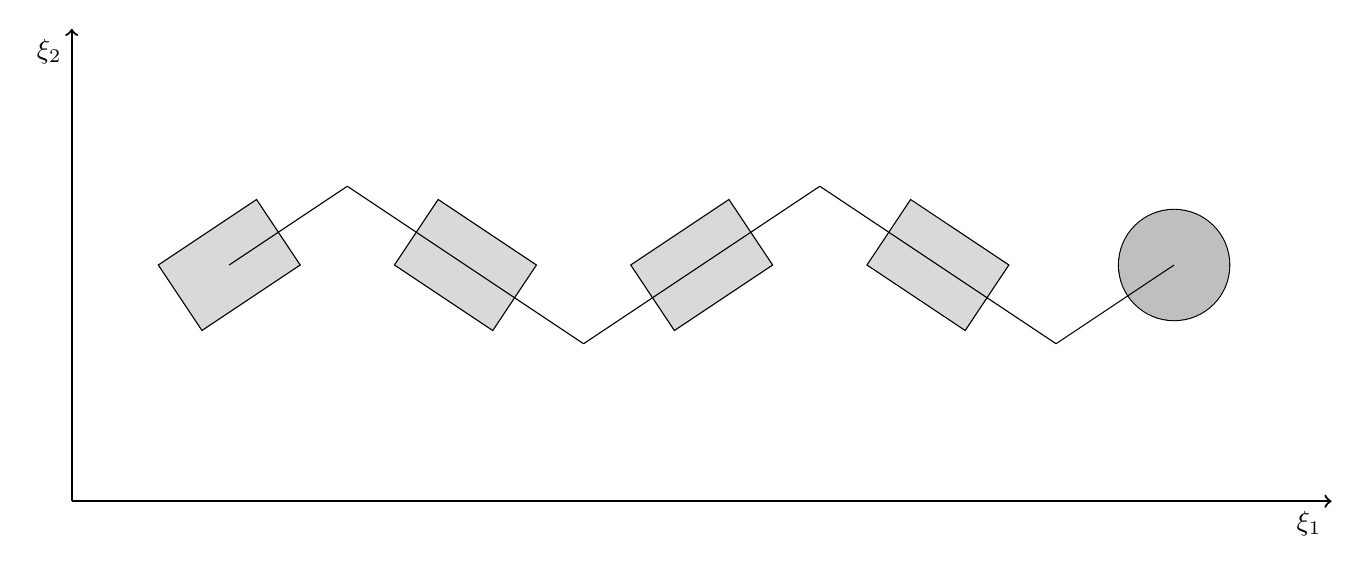
\begin{tikzpicture}
			%[extended line/.style={shorten >=-#1,shorten <=-#1},
			%extended line/.default=1cm,	one end extended/.style={shorten >=-#1}]
			
			% Koordinatensystem
			\draw[thick,->] (0,0) -- (16,0) node[anchor=north east] {$ \xi_{1} $};
			\draw[thick,->] (0,0) -- (0,6)  node[anchor=north east] {$ \xi_{2} $};
			% Fahrzeuge
			\coordinate (x0) at (14,3);
			\coordinate (d0) at (12.5,2);
			\coordinate (x1) at (11,3);
			\coordinate (d1) at (9.5,4);
			\coordinate (x2) at (8,3);
			\coordinate (d2) at (6.5,2);
			\coordinate (x3) at (5,3);
			\coordinate (d3) at (3.5,4);
			\coordinate (x4) at (2,3);
			\pgfmathanglebetweenpoints{\pgfpointanchor{d0}{center}}{\pgfpointanchor{x1}{center}}
			\edef\angP{\pgfmathresult}
			\pgfmathanglebetweenpoints{\pgfpointanchor{d1}{center}}{\pgfpointanchor{x2}{center}}
			\edef\angN{\pgfmathresult}			
			
			\draw[thick] (x0) circle(0.7cm);
			\fill[gray!50] (x0) circle(0.7cm);
			
			\node [draw, rotate=\angP, shape=rectangle, minimum width=1.5cm, minimum height=1cm, anchor=center, fill=gray!30] at (x1) {};
			\node [draw, rotate=\angN, shape=rectangle, minimum width=1.5cm, minimum height=1cm, anchor=center, fill=gray!30] at (x2) {};
			\node [draw, rotate=\angP, shape=rectangle, minimum width=1.5cm, minimum height=1cm, anchor=center, fill=gray!30] at (x3) {};
			\node [draw, rotate=\angN, shape=rectangle, minimum width=1.5cm, minimum height=1cm, anchor=center, fill=gray!30] at (x4) {};
			
			\draw (x0) -- (d0);
			\draw (d0) -- (x1) -- (d1);
			\draw (d1) -- (x2) -- (d2);
			\draw (d2) -- (x3) -- (d3);
			\draw (d3) -- (x4);
			
		\end{tikzpicture}


\section{\textcolor{red}{Regelstrukturen}}
	\subsection{\textcolor{red}{Kaskadenregelung}}
		
\section{\textcolor{red}{Vektorregelung}}

\subsection{Adaptive Regelung}
\part{Informatik}
\section{Matlab}
\part{Berühmte Wissenschaftler}
\addsec{15'th century}
\subsection{Leonardo da Vinci 			1452-1519}
\subsection{Nikolaus Kopernikus 		1473-1543}
\addsec{16'th century}
\subsection{Galileo Galilei 			1564-1642}
\subsection{Johannes Keppler 			1571-1630}
\addsec{17'th century}
\subsection{Isaac Newton 				1643-1727}
\addsec{18'th century}
\subsection{Carl Friedrich Gauß 		1777-1855}
\subsection{Michael Faraday 			1791-1867}
\addsec{19'th century}
\subsection{Charles Darwin 			1809-1882}
\subsection{Gustav Robert Kirchhoff    1824-1887}
\subsection{James Clerk Maxwell 		1831-1879}
\subsection{Thomas Alva Edison 		1847-1931}
	Wer der Erfinder der Glühbirne ist, ist nach wie vor ein Rätsel. Anscheinend soll der deutsche Uhrenmacher Heinrich Göbel im Jahre 1854 die erste Glühlampe gebaut und erfunden haben. Jedoch verfügte dieser weder über das Know-How noch die technischen Geräte um ein derartiges Projekt fertigzustellen. 1879 hat Edison eine Kohlefaden-Lampe gebaut und darauf ein Patent erhalten. Wer aber die Idee dazu ist unbekannt.
	\begin{itemize}
		\item Thomas Edison meldete für über tausend Erfindungen Patente an
		\item Edison galt als skrupelloser Geschäftsmann
		\item Er versuchte den Gleichstrom bei der Elektrifizierung für seinen eigenen Profit durchzusetzen, gewonnen hat der Wechselstrom von Westinghouse. Er richtete sogar öffentliche Tiere durch Wechselstrom hin um zu zeigen, dass dieser gefährlich sei und sein Gleichstrom nicht. Als Höhepunkt brachte er einen Elefanten um.
	\end{itemize}
\subsection{Nikola Tesla 				1856-1943}
	Ausbildung: Technische Universität Graz\\
	Herkunft: Serbien\\
	In Österreich bis 1891 gelebt, danach bis zum Tod in Amerika. \\\\
	\textbf{Erfindungen:}
	\begin{itemize}
		\item Drehstrom-Asynchronmaschine
		\item rotierendes magnetisches Feld
		\item Tesla-Spule (el. Energie durch Luft übertragen: hochspannung, niedrgier Strom, hohe Frequenz)
		\item erstes ferngesteuertes Boot
	\end{itemize}
	
\subsection{Heinrich Hertz 			1857-1894}
\subsection{Max Planck 				1858-1947}
\subsection{Albert Einstein 			1879-1955}
\subsection{Niels Bohr 				1885-1962}
\addsec{20'th century}
\subsection{Werner Heisenberg 			1901-1976}
\subsection{Stephen Hawking 			1942-heute}





	

\end{document}